\documentclass{article}
\usepackage{ctex} 
\usepackage{graphicx}  
\usepackage{booktabs}     
\usepackage{amsmath}
\usepackage{changepage}   
\usepackage{caption}     
\usepackage[style=authoryear,backend=biber]{biblatex}
\addbibresource{ref.bib}  
\usepackage{float}
\usepackage{tabularx}
\usepackage{threeparttable}

\title{北向资金对A股市场的影响与基于北向资金的量化交易策略 -- 中期报告}
\author{杨明宸}
\date{\today}

\begin{document}
\maketitle

\tableofcontents
\newpage

\listoffigures
\newpage

\listoftables
\newpage

\begin{abstract}

\textbf{中文摘要}

自沪港通于2014年正式开通以来，以北向资金为代表的境外投资者日益深度参与中国A股市场，其规模与市场影响力持续扩大。然而，受制于历史数据积累不足，学术界对北向资金的系统性实证研究至今仍相当匮乏。本文以沪市A股为研究对象，基于2017年至2025年间的逐股日度持仓与行情数据，从学术与工业双重视角对北向资金展开全面分析：

在北向资金自身特征方面，本文首先通过构建修正相关系数并进行HAC稳健t检验，证实北向资金交易具有显著且稳健的超额收益能力。进一步将收益分解为选股收益与择时收益，发现二者贡献分别约为42\%与58\%，以择时为主。在交易模式上，本文构造了适用于非对称买卖场景的交易率指标，实证表明北向资金的换手率远高于本土机构投资者，甚至接近散户水平，呈现出"对冲基金式"的高频交易特征。与此对应，本文通过不同预测周期下的相关系数检验发现，北向资金仅对短期价格波动（一周至一个月）具有统计显著的预测能力，对半年乃至更长期回报无显著预测力。

在北向资金对A股市场的影响方面，本文做出了两项重要实证贡献。其一，通过VAR建模与脉冲响应函数分析，发现北向资金净流入可引发持续约一周的市场羊群效应。其二，本文\textbf{首次}系统检验了允许北向资金交易对个股收益波动率的系统性影响：以沪港通开通为准自然实验，采用双重差分法（DID）并控制个体与时间固定效应，实证发现被纳入沪港通的股票在政策实施后波动率显著系统性提高，且这一结论在剔除事件窗口临近期数据、加入多维财务控制变量及行业哑变量后依然稳健。上述两项发现共同表明，北向资金对A股市场价格发现功能的促进作用有限，其高频交易行为反而可能加剧市场短期波动。

在量化策略构建方面，针对A股因涨跌停板与卖空限制导致动量反转效应产生大量虚假alpha这一问题，本文通过构造"类Barra"残差化目标（剔除市场、行业、市值及多维动量反转因子的线性影响）来规避上述陷阱，所得策略alpha与传统动量反转alpha在统计上完全独立。在此基础上，本文设计了二十余个针对北向资金持仓变动特征的工程化特征，并采用增量式滚动岭回归进行训练。样本外回测显示，线性模型实现了年化约14.5\%的超额收益与接近5.0的夏普比率，alpha自相关结构与北向资金的高频交易特征高度吻合，印证了策略的经济逻辑自洽性。进一步引入LightGBM与CatBoost两类非线性树模型进行测试，结果表明在当前信噪比与特征维度约束下，非线性模型样本外表现相较线性模型并无显著增益，提示alpha的可预测成分在现有特征框架下主要为线性结构。

\textbf{关键词}：北向资金；陆港通；A股市场；价格波动率；双重差分；量化交易策略；动量反转；滚动岭回归

\newpage

\textbf{Abstract}

Since the launch of the Shanghai-Hong Kong Stock Connect (Northbound Connect) in November 2014, northbound capital — foreign investors accessing China's A-share market through the Stock Connect schemes — has grown substantially in scale and market influence. Yet, owing to the limited accumulation of historical data, systematic empirical research on northbound capital remains scarce. This paper employs daily stock-level position and market data for Shanghai A-shares from 2017 to 2025 to conduct a comprehensive analysis of northbound capital from both academic and practitioner perspectives.

Regarding the characteristics of northbound capital, we first construct a modified cross-sectional correlation coefficient and conduct HAC-robust t-tests, establishing that northbound trading generates statistically significant and robust excess returns. Decomposing returns into stock-selection and market-timing components yields contributions of approximately 42\% and 58\%, respectively, indicating a predominantly timing-driven profit source. In terms of trading behavior, we develop a turnover rate measure suited to the asymmetric buy/sell structure of Stock Connect participation, and find that northbound investors trade far more frequently than domestic institutional investors — approaching the turnover level of retail investors — consistent with a hedge-fund-style, high-frequency trading pattern. Correspondingly, cross-period predictive correlation tests reveal that northbound capital exhibits statistically significant return predictability only at short horizons (one week to one month), with no meaningful predictive power at half-year or longer horizons.

Concerning the impact of northbound capital on the A-share market, we make two key empirical contributions. First, using VAR modeling and impulse response analysis, we find that northbound net inflows trigger a herd-following effect in aggregate market trading that persists for approximately one week. Second, this paper \textbf{is the first} to systematically examine the effect of Stock Connect inclusion on individual stock return volatility: treating the launch of the Shanghai-Hong Kong Stock Connect as a quasi-natural experiment and employing a difference-in-differences (DID) estimator with individual and time fixed effects, we find that stocks admitted to the Stock Connect experience a significant and systematic increase in return volatility after the policy. This finding is robust to excluding data in the windows immediately surrounding the event, to the inclusion of multi-dimensional financial control variables, and to industry fixed effects. Taken together, these results suggest that northbound capital contributes little to the price discovery function of A-shares, and that its high-frequency trading behavior may instead amplify short-term market volatility.

On the quantitative strategy side, we address the well-known problem in A-share markets whereby momentum/reversal effects generate spurious alpha due to short-selling constraints and daily price limits. We construct a ``Barra-style'' residualized return target that strips out the linear contributions of market, industry, size, and multi-horizon momentum/reversal factors, ensuring that the resulting alpha is statistically orthogonal to conventional momentum/reversal strategies. Building on this framework, we engineer over twenty features capturing dynamics in northbound capital position changes, and train an incremental rolling ridge regression. Out-of-sample backtests show that the linear model achieves an annualized excess return of approximately 14.5\% and a Sharpe ratio close to 5.0; the autocorrelation structure of the alpha signal closely mirrors the high-frequency trading profile of northbound capital, confirming the internal economic consistency of the strategy. We further test LightGBM and CatBoost nonlinear tree models, finding no significant out-of-sample improvement over the linear baseline under the current signal-to-noise ratio and feature dimensionality constraints, suggesting that the predictable component of alpha is predominantly linear within the existing feature framework.

\textbf{Keywords}: Northbound Capital; Stock Connect; A-Share Market; Return Volatility; Difference-in-Differences; Quantitative Trading Strategy; Momentum/Reversal; Rolling Ridge Regression

\end{abstract}

\newpage

\section{引言}

如本文标题所示，我们的研究主题是从学术视角与工业视角双重分析北向资金的特征：从学术视角入手，我们希望了解北向资金的盈利能力，收益来源，交易特征等，进而通过实证验证回答陆港通开通十余年来，北向资金的引入对A股股票到底产生了什么影响——
北向资金是确实发现了A股市场中被低估的投资机会，提升了A股市场的价格发现功能，还是利用了A股的情绪波动实现收益？引入北向资金是加强了A股的价格发现功能，还是加剧了市场波动？
而从工业视角入手，我们希望基于对北向资金特征的理解，构建一个基于北向资金信息的量化交易策略，并通过实证分析验证该策略的有效性。

\subsection{研究背景与研究意义}

自2014年11月17日沪港通正式开通以来，以北向资金为代表的境外投资者获得了直接参与中国A股市场的制度性通道。随后，深港通于2016年12月启动，两项制度合称"陆港通"，共同构成了中国资本市场对外开放的重要基础设施。截至2023年末，沪深港通北向持股总市值已超过2.3万亿元人民币，占A股流通市值比例约3.5\%，而其日均成交占比则长期维持在全市场的10\%至15\%之间，在活跃交易层面的存在感远超其持仓权重。\footnote{数据来源：上海证券交易所、深圳证券交易所年度统计报告及东方财富Choice终端。}

从宏观背景来看，北向资金的持续壮大有其深刻的制度逻辑与市场背景。一方面，中国经济体量的持续扩张使A股市场在全球资本配置版图中的战略地位日益凸显：2020年，中国GDP首次突破100万亿元人民币，A股总市值也跻身全球第二大股票市场之列。另一方面，A股被全球主要指数相继纳入——MSCI于2018年首次将A股纳入其新兴市场指数，富时罗素与标普道琼斯指数随后跟进——这使得全球被动配置资金对A股的需求结构性上升，进一步强化了北向资金规模扩张的长期趋势。

然而，在北向资金规模与影响力持续攀升的同时，市场对其性质与行为模式的认识却存在相当程度的模糊与分歧。一方面，监管部门在设计沪港通制度时，明确将"引入富有投资经验的境外资金、促进A股市场价格发现功能完善"列为政策目标之一，这一表述在学术界和工业界逐渐演化为对北向资金"聪明钱（smart money）"身份的广泛默认。另一方面，现实中亦多次出现北向资金大幅流出与A股剧烈波动相互叠加的场景——典型案例如2023年8月，在宏观预期悲观的背景下，北向资金在数周内累计净流出近600亿元，被广泛视为市场信心受损的重要表征，由此引发了监管层对信息披露机制的反思，并最终导致2023年8月北向资金实时交易数据的公开暂停。

上述现实张力表明，北向资金对A股市场的影响远非"价值发现"这一单一叙事所能概括，其中涉及的核心问题——北向资金的盈利能力从何而来？其交易频率与行为模式究竟与哪类投资者更为相似？它对A股市场究竟是增进了价格发现效率，还是加剧了短期波动？——均需要基于扎实的实证数据和严格的统计方法加以回答。

正是在这一背景下，本文的研究具有重要的学术价值与现实意义。从学术价值而言，现有针对中国资本市场外资行为的实证研究数量有限，且多依赖指数级别汇总数据，难以揭示个股层面的微观机制；而已有研究所得出的结论之间也存在相互矛盾之处，亟需更长时间跨度、更细粒度的数据加以厘清。从现实意义而言，随着中国资本市场双向开放进程的深化，准确评估境外资本参与的市场效应，对于监管政策的精准制定、投资者的理性预期形成以及市场稳定机制的健全完善，均具有相当的参考价值。

\subsection{研究对象与目标}

本文的研究对象为通过沪港通渠道进入沪市A股市场的北向资金，研究区间为2017年10月至2025年10月，核心数据为个股层面的日度持仓明细与行情数据。之所以选择沪市而非深市，主要基于以下考量：其一，沪港通开通时间（2014年）早于深港通（2016年），历史数据积累更为充分；其二，沪市大盘蓝筹股集中，具有更好的代表性；其三，可用数据的完整性在沪市方面更有保障，有助于实证结论的稳健性。

本文的研究目标可分为学术目标与工业目标两个层面：

\textbf{学术目标方面}，本文旨在从严格的实证视角回答以下三组问题：
\begin{enumerate}
    \item \textbf{北向资金的自身特征}：北向资金是否具有统计显著且经济实质性的超额收益能力？其收益主要来源于横截面选股能力还是时间序列择时能力？其换手率与交易频率在与本土机构投资者及散户投资者的比较中处于何种水平？
    \item \textbf{北向资金对A股收益率的影响}：北向资金的净流入是否会对个股未来收益率产生格兰杰因果效应？二者之间是否存在统计显著的短期羊群效应？
    \item \textbf{北向资金对A股波动率的影响}：北向资金的日频净交易量是否对个股收益波动率具有显著的预测或因果效应？允许北向资金参与交易是否会系统性地改变个股的长期波动率水平？
\end{enumerate}

\textbf{工业目标方面}，本文旨在基于上述学术分析所揭示的北向资金行为特征，构建一套具有可交易价值的量化交易策略。具体而言，我们将着重解决A股市场因卖空限制和涨跌停板机制产生的虚假动量alpha问题，通过构造"类Barra"残差化目标，设计针对北向资金持仓变动特征的工程化特征，并在线性模型框架下进行增量滚动训练与样本外回测，同时引入非线性树模型对alpha的极限性能进行测试。

\subsection{研究创新点}

本文的主要创新贡献体现在以下五个方面：

\textbf{第一，量化了北向资金盈利能力的择时来源与选股来源贡献。}现有文献在衡量北向资金的盈利能力时，普遍沿用标准截面相关系数，但该指标会损失时序择时收益的信息。本文提出的修正相关系数（式\ref{eq:tilde_coef}）通过移除截面均值去中心化操作，同时捕捉了选股和择时两类收益来源，并在HAC稳健框架下完成假设检验。与此同时，针对沪港通买卖可与大陆本土投资者对向交易的制度特征，本文设计了适配非对称买卖结构的交易率指标（式\ref{eq:my_turnover}），使北向资金换手率与市场整体换手率的比较具备了方法论上的可比性。

\textbf{第二，以沪港通开通为准自然实验，系统识别了北向资金引入对个股收益率与波动率的因果效应。}本文利用2014年11月17日沪港通正式开通这一外生政策冲击，构建了一套完整的准自然实验框架：一方面，通过VAR建模与脉冲响应函数分析，在收益率层面识别出北向资金净流入引发约一周持续的市场羊群效应；另一方面，采用双重差分（DID）方法并控制个体固定效应与时间固定效应，在波动率层面首次系统地识别出"被纳入沪港通"这一处理变量对个股长期波动率的正向因果效应。上述两项识别策略均在剔除事件窗口临近期数据、引入多维财务控制变量及行业哑变量后保持稳健，共同揭示了北向资金引入对A股市场价格行为的系统性影响。

\textbf{第三，提出并实现了一套完整的针对A股特殊制度约束的alpha残差化框架，并产出了与动量反转策略正交的超额收益夏普比率接近5.0、IC达1.2的高质量可交易alpha。}A股市场因卖空限制与涨跌停板制度，导致传统动量反转因子产生大量名义上显著但实际上无法交易的虚假alpha。本文通过构建包含市场因子、行业因子、市值因子和多时间尺度动量反转因子的"类Barra"残差化体系，在训练目标层面彻底剔除这些虚假alpha成分，使得后续策略所展示的alpha与所有动量反转策略在统计上完全正交，从而保证了超额收益的可交易性与来源可解释性。在此框架下，基于北向资金持仓特征的滚动Ridge回归策略在样本外实现了年化约14.5\%的超额收益、夏普比率接近5.0以及ICIR达1.2的优异表现，充分证明了残差化alpha的实际投资价值。

\textbf{第四，通过线性模型与非线性模型的系统对比，揭示了当前特征框架下北向资金alpha可预测成分的结构特征。}本文通过LightGBM与CatBoost两类非线性树模型的测试，发现在当前信噪比与特征维度约束下，非线性模型无法带来样本外的显著增益，由此得出该alpha的可预测成分在现有特征框架下主要为线性结构这一结论，并从统计学习理论视角对这一现象给出了系统性解释。

\subsection{论文结构}

本文共分为六个部分，各部分之间在逻辑上形成"特征刻画—影响识别—策略构建"的递进关系。

第一部分为引言，阐明研究背景与动机，界定研究对象与目标，概述主要创新贡献，并说明论文结构安排。

第二部分为文献综述，从北向资金交易行为特征、北向资金对A股个股的影响以及利用北向资金构造交易策略三个维度系统梳理国内外相关研究，在此基础上指出现有文献的不足，从而明确本文的研究定位。

第三部分为数据说明，对本文使用的全部数据的来源、时间范围、频率及覆盖范围进行系统介绍，并对关键数据的处理方式加以说明。

第四部分为实证方法与结果，是本文的核心内容，分为两个相互关联的子模块。第一子模块聚焦北向资金自身特征，依次考察其超额收益能力（4.1.1节）、收益来源分解（4.1.2节）、交易模式（4.1.3节）以及对证券长短期回报的相对预测能力（4.1.4节）。上述分析共同揭示出北向资金具有显著超额收益、以择时为主要盈利来源、换手率接近散户水平、且仅对短期价格波动具有预测力等核心特征，从而为第二子模块提供了研究假说。第二子模块聚焦北向资金对A股市场的影响，依次检验其对股票收益率的格兰杰因果效应与羊群效应（4.2.1节），讨论收益波动率的合理度量方法（4.2.2节），通过VAR与脉冲响应函数分析北向资金净流入对波动率的短期因果关系（4.2.3节），并以沪港通开通为准自然实验，采用双重差分法系统识别北向资金准入对个股波动率的系统性长期影响（4.2.4节）。两个子模块在逻辑上构成从"北向资金是什么"到"北向资金做了什么"的完整因果链条。

第五部分为策略设计与回测分析，以第四部分揭示的北向资金特征为出发点，依次介绍目标残差化框架与特征工程（5.1节）、基于增量式滚动Ridge回归的线性模型设计与算法（5.2节）、评价指标及样本外回测结果（5.3节），以及引入LightGBM与CatBoost对alpha极限性能的测试与讨论（5.4节）。

第六部分为总结，对全文主要实证发现进行归纳，并指出研究的局限性与未来可能的改进方向。

\newpage
\section{国内外相关研究综述}

围绕北向资金（沪深港通北向资本流动）的交易行为、市场效应与策略价值，
国内外学术界已积累了相当数量的文献。然而，正如下文所梳理的，
现有研究在研究方法、样本选取与因果识别等方面均存在明显局限，
尤其是国内研究结论相互矛盾，研究空白依然显著，
这为本文的系统性研究提供了充分的学术动机。

% ──────────────────────────────────────────
\subsection{北向资金交易行为特征}
% ──────────────────────────────────────────

对北向资金交易行为的刻画是理解其市场影响的基础前提。
\cite{JTJJ202212008}以沪港通开通为准自然实验，
发现北向资金的引入显著提升了标的股票的市场流动性；
\cite{JRQH202109017}进一步指出，北向资金的持续注入不仅为A股市场带来了增量资金，
也为本地市场参与者提供了更多元的投资机会，从而整体上促进了市场流动性与活跃度。
然而，上述两项研究所记录的流动性提升也可以被理解为情绪化波动的加剧，
即北向资金在改善市场深度的同时，也可能放大短期价格噪声，两种解读均有一定文本支持。

在信息传导机制方面，\cite{TODEA201334}基于欧洲市场数据实证表明，
国际资本参与与本国股市信息透明度之间存在相互促进的正向循环：
一国信息透明度越高，国际资本参与越充分，而这进一步强化了市场的信息效率。
这一发现为研究北向资金对A股信息环境的影响提供了重要的理论参照。

然而，北向资金对市场流动性的影响并不是单向的。
\cite{ZYCY202303004}指出，北向资金具有显著的"鲇鱼效应"，
其对高盈余质量股票的偏好倒逼公募基金向同方向集中配置，
这一结构性压力客观上降低了小市值股票的流动性。
\cite{STYS20231207004}则从风险配置角度提供了补充证据，
认为北向资金能够降低市场对骑士风险（Knight uncertainty）的资金暴露，
其实质同样是引导资金远离小市值标的，进一步压缩了该类股票的流动性深度。
上述发现揭示出北向资金交易行为的结构性异质性：
其流动性效应因标的市值规模和盈余质量的不同而呈现出显著差异，
而非文献早期所描绘的普惠式改善。

在交易模式识别方面，\cite{经管实证}对北向资金的交易特征进行了系统研究，
发现其交易者整体上呈现出动量效应，即倾向于追涨杀跌。
这一发现具有重要的方法论含义：如果北向资金本身是动量策略的执行者，
那么其资金流动与同期收益率之间的正相关关系，在相当程度上可能反映的是
动量因子的暗含作用，而非北向资金所独立携带的信息含量。
这一逻辑漏洞在后续策略研究中尤为关键，详见第\ref{sec:strategy}节。

% ──────────────────────────────────────────
\subsection{北向资金对A股个股的影响}
\label{subsec:impact}
% ──────────────────────────────────────────

\subsubsection{收益率层面}

在收益率预测能力方面，国外研究提供了相对一致的参照基准。
\cite{doi:10.1080/23322039.2020.1754321}对外国证券投资对印度股市的影响进行了系统分析，
指出外国投资者对证券未来收益不具备显著的预测能力，但外国资金净流入与短期收益波动率之间
存在显著正相关关系。该研究还发现，资金净流入与净流出之间存在非对称效应：
利用TGARCH模型的分析表明，资金净流出更易引发羊群效应；
而对于小公司，非预期资金流入会导致波动率的显著上升，
但对大中型公司而言这种效应并不显著。
\cite{CHAKRABARTI20021}利用1997年东亚金融危机期间的印度数据得出，
投资资金净流入与中长期证券回报无显著相关关系；
\cite{CHOE1999227}、\cite{RePEc:bin:bpeajo:v:29:y:1998:i:1998-2:p:137-206}
和\cite{KIM200277}等研究也在不同国家和不同市场背景下得出了类似的结论。
综合来看，国外文献较为一致地表明，外国投资者通常不具备显著的超额收益能力，
其资金流动更多反映了跟随市场的趋势交易行为。

\cite{ctx3501173690004886}从理论上解释了外国投资者跑输本国投资者的内在机制：
外国投资者因对本地股票信息了解不足，在信息匮乏条件下更易发生趋同交易，
其在羊群效应中扮演"从羊"角色的概率显著高于本国投资者；这一理论推断得到了实证支持。

在A股市场的研究中，\cite{RePEc:eee:finlet:v:56:y:2023:i:c:s1544612323005470}
指出北向资金可通过提升股价信息效率与改善公司治理质量来提高本地市场效率；
\cite{123}则通过基础性实证分析得出北向资金是"聪明的钱"这一结论，
认为其具备一定的信息优势。然而，这些结论与其他研究之间的张力始终未能得到妥善处理。

\subsubsection{波动率层面}

波动率效应方面，现有文献的分歧尤为突出，堪称该领域研究中矛盾最为集中之处。
\cite{YNJR201532099}的实证研究验证了北向资金的引入显著增加了标的股票的波动率；
\cite{JRYJ201807011}的结论则截然相反，认为北向资金显著降低了标的的波动率；
而\cite{JKJS201710022}的研究结果显示，北向资金对波动率没有显著影响。
三项研究的结论几乎覆盖了所有可能的方向性结论，而彼此之间在方法论层面缺乏可比性对照。

上述分歧的根源在于三个方面：第一，现有研究大多采用时序相关分析或事件研究方法，
缺乏能够剥离选择偏差的因果识别工具；第二，绝大多数研究未区分北向资金标的与非标的之间
因系统性差异（市值、行业、流动性）造成的混淆效应；
第三，部分研究的样本期横跨沪港通开通前后，将事件本身的冲击混入了常态期的效应估计。
这些方法论缺陷使得现有文献在波动率效应这一核心问题上至今无法形成共识。

% ──────────────────────────────────────────
\subsection{利用北向资金构造交易策略}
\label{subsec:strategy}
% ──────────────────────────────────────────

在策略研究方面，现有文献数量有限，且普遍存在严重的方法论缺陷。

\cite{1021514008.nh}尝试利用北向资金的历史持仓数据构建交易策略，
所呈现的策略回测表现颇为亮眼。然而该研究存在一个根本性的数据使用缺陷：
北向资金的持仓数据在制度层面属于盘后公布，即投资者在当日收盘后方能获取当日持仓变动；
而该研究在策略构建中将当日持仓变动与当日收益率同期对齐使用，
实质上造成了数据泄露（look-ahead bias）。
剔除这一信息超前效应后，策略的盈利能力是否依然存在，该研究并未给出说明。
更重要的是，北向资金持仓变动与同期收益率之间的高度相关性本身正是值得警惕的信号：
如图\ref{fig:causality}所示，这种相关性既可能来源于北向资金对价格的真实信息引导，
也可能仅仅是动量反转效应的另一种表达——即北向资金本身追涨杀跌，
其持仓变动与价格变动之间的相关性是策略的表象，而非策略的来源。
若不对这种混淆效应加以剥离，策略的alpha来源便无从辨别。

\begin{figure}[htbp]
    \centering
    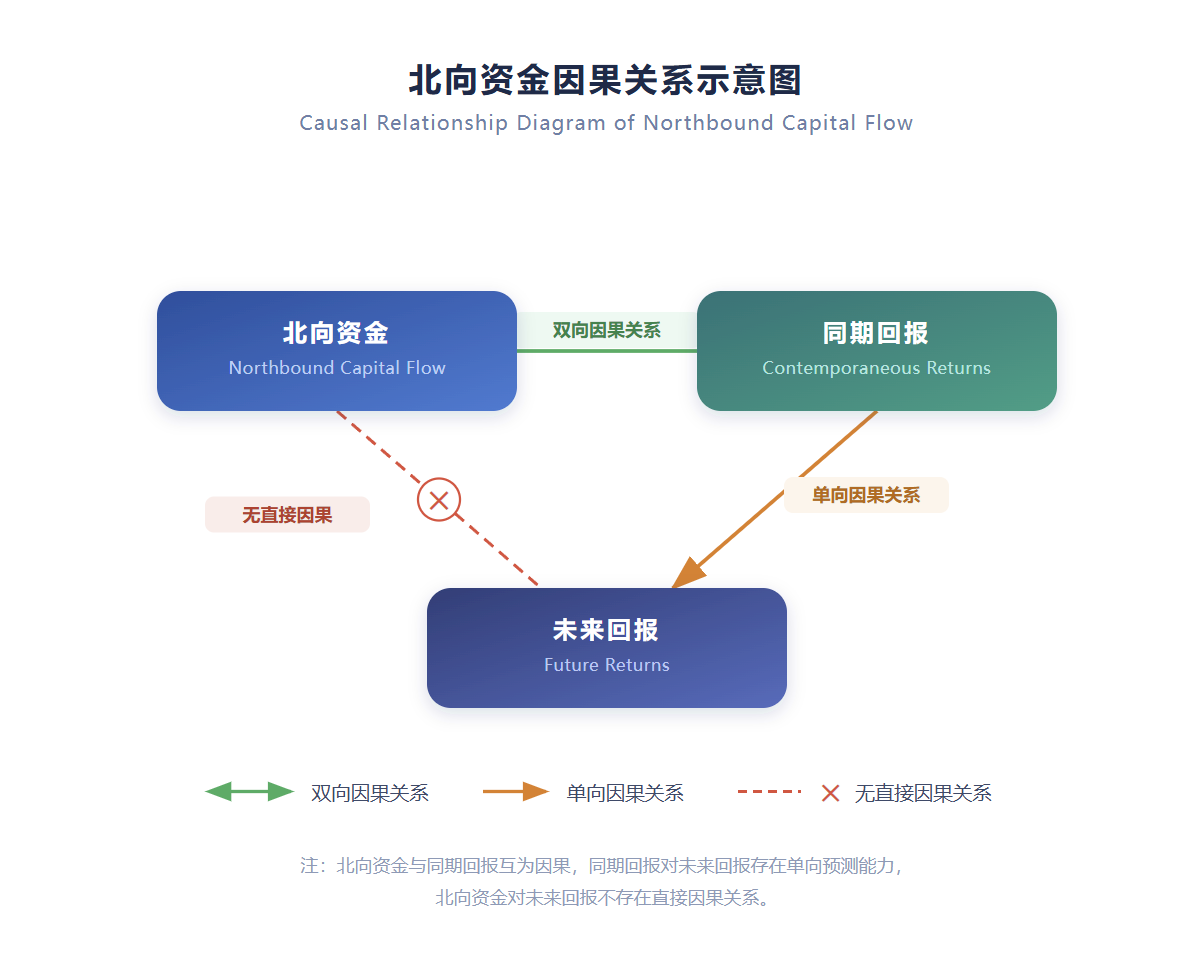
\includegraphics[width=0.72\textwidth]{../Figure/因果关系示意图.png}
    \caption{北向资金持仓变动与股价收益率的相关性来源示意图。
    相关性可能来自北向资金独立携带的信息（真实alpha通道），
    也可能来自二者共同受动量反转效应驱动（虚假alpha通道）。
    未对两条通道加以区分时，策略的alpha来源不可解释。}
    \label{fig:causality}
\end{figure}

\cite{经管策略}在沪深300成分股范围内构建了利用北向资金的量化选股策略，
并得到了一定程度的正向回测结果。然而该研究存在两个突出局限：
其一，选股范围局限于沪深300，样本仅涵盖A股中大市值的头部公司，
泛化能力存疑；其二，策略未对动量反转效应加以控制，
无法判断所记录的超额收益究竟来自北向资金的信息增量，
还是动量因子在特定样本期的溢价。这两项局限导致该策略的实际可应用性大打折扣。

综合来看，现有策略研究存在以下共性缺陷：
未剔除数据泄露、未控制动量反转因子暴露、样本范围受限，
以及缺乏对alpha来源的统计分解与可解释性分析。

% ──────────────────────────────────────────
\subsection{现有文献局限与本文研究目标}
\label{subsec:gap}
% ──────────────────────────────────────────

通过对上述文献的系统梳理，现有研究存在以下四个层面的主要局限：

\textbf{第一，盈利能力度量方法存在信息损失。}
现有文献在衡量北向资金的盈利能力时，普遍采用标准截面相关系数（IC），
该指标通过截面去均值化操作压缩了时序择时收益的信息，
使得选股贡献与择时贡献无法被独立识别。与此同时，现有研究所使用的换手率指标
通常未考虑沪港通制度下买卖双方非对称参与的结构性特征，
导致北向资金的交易强度估计与A股整体换手率之间缺乏可比的方法论基础。

\textbf{第二，因果识别工具缺位，相关关系与因果效应混淆。}
波动率效应领域三项主要研究得出三种截然相反结论这一现象，
其根本原因在于均采用相关分析或普通面板回归，
缺乏能够剥离个体固定效应、时间趋势与选择偏差的因果识别框架。
在未引入外生政策冲击作为准自然实验的前提下，
北向资金流动与个股价格行为之间的关系始终处于相关而非因果的讨论层面。

\textbf{第三，策略研究存在系统性数据泄露与因子混淆。}
现有策略研究或因忽视北向持仓盘后公布的制度约束而引入未来信息，
或因未控制动量反转因子暴露而无法甄别alpha的真实来源，
使得所报告的策略表现不具备实盘可复制性与来源可解释性。

\textbf{第四，研究结论的泛化能力受限，全市场视角缺失。}
现有策略研究普遍局限于沪深300等大市值样本，
对北向资金在中小市值股票中的行为特征与信息含量缺乏系统考察，
而这恰恰是北向资金对市场结构影响最显著的区域。

针对上述局限，本文的研究目标可概括如下：
第一，在方法论层面，提出修正相关系数与适配非对称买卖结构的换手率指标，
实现北向资金盈利能力的精确分解；
第二，以沪港通开通为外生政策冲击，构建完整的准自然实验框架，
在收益率和波动率两个层面分别实现北向资金影响的因果识别；
第三，建立包含多尺度动量反转因子的"类Barra"残差化框架，
彻底剥离A股制度性因子对策略alpha的污染，
并在此框架下产出与动量反转策略统计正交的可交易超额收益；
第四，通过线性与非线性模型的系统对比，
揭示当前特征框架下北向资金alpha可预测成分的结构特征，
为后续研究提供方法论参照。

\newpage
\section{数据来源}

我们将本文中使用到的所有数据汇总为下面一张表格：

\begin{table}[!ht]
    \label{tab:data_summary}
    \centering
    \small  % 可选：稍微缩小字体以适应更多内容
    \begin{tabularx}{\textwidth}{|X|l|l|l|l|X|}
    \hline
    \textbf{数据名称} & \textbf{数据来源} & \textbf{起始时间} & \textbf{终止时间} & \textbf{更新频率} & \textbf{数据范围} \\ \hline
    陆港通持股仓位明细 & CSMAR & 2017.10.09 & 2025.10.08 & 日频 & 陆港通标的 \\ \hline
    A股行情数据 & CSMAR & 2017.10.09 & 2025.10.08 & 日频 & A股 \\ \hline
    沪市A股交易金额占比 & CEIC数据库 & 2007.12 & 2017.12 & 年频 & 汇总 \\ \hline
    沪市A股持股金额占比 & CEIC数据库 & 2007.12 & 2022.12 & 年频 & 汇总 \\ \hline
    沪港通净买入金额 & CEIC数据库 & 2017.03 & 2023.11 & 日频 & 汇总 \\ \hline
    沪港通净卖出金额 & CEIC数据库 & 2017.03 & 2023.11 & 日频 & 汇总 \\ \hline
    沪市A股换手率 & CEIC数据库 & 2017.03 & 2023.11 & 日频 & 汇总 \\ \hline
    陆港通样本股纳入纳出 & CSMAR & 2014.05 & 2015.05 & 一次性 & 陆港通标的 \\ \hline
    A股公司行业代码 & CSMAR & NA & NA & 一次性 & A股 \\ \hline
    A股公司财务报表 & CSMAR & NA & NA & 一次性 & A股 \\ \hline
    \end{tabularx}
    \caption{数据来源与描述}
\end{table}

\subsection*{数据说明}

本文共使用十类数据，以下按数据来源与用途分别加以介绍。

\textbf{陆港通持股仓位明细}（CSMAR，2017.10.09—2025.10.08，日频，覆盖全部陆港通标的）是本文最核心的数据。该数据记录了每个交易日收盘时北向资金对各标的股票的持仓金额，通过对相邻交易日持仓金额求差，可以估算北向资金对每只股票的每日净流入（净买入金额）。这一数据被用于第\ref{sec:strategy}节中绝大多数的实证分析：在4.1.1节中用于估算北向资金的累积绝对收益与交易相对收益；在4.1.2节中进行收益来源分解（选股收益与择时收益）；在4.1.3节中计算北向资金的交易率；在4.1.4节中检验北向资金对证券不同预测周期下的相关系数；在4.2.1节中构建VAR模型检验北向资金净流入对市场成交额的格兰杰因果关系；在4.2.3节中分析北向资金净流入对股票收益波动率的短期影响；在第五节策略设计中作为特征工程的原始字段之一（北向资金净持仓变动）。

\textbf{A股行情数据}（CSMAR，2017.10.09—2025.10.08，日频，覆盖全A股）包含个股每日的开盘价、收盘价、最高价、最低价及成交金额等字段。该数据与陆港通持股仓位明细配合，在4.1.1节中用于计算各股票的CloseToClose日收益率，从而估算北向资金持仓的绝对收益与交易相对收益；在4.1.3节中计算全市场的换手率，作为与北向资金交易率进行比较的基准；在4.2.1节中提供沪港通标的股的每日总成交金额用于VAR建模；在4.2.2节和4.2.3节中用于计算两种波动率指标（$Vol_1$和$Vol_2$）；在4.2.4节的DID分析中用于计算实验窗口内各股票的日度波动率；在第五节策略回测中用于计算各股票的对数收益率（残差化目标的原始输入）并提供流通市值数据用于权重构造。

\textbf{沪市A股交易金额占比}和\textbf{沪市A股持股金额占比}（CEIC数据库，分别覆盖2007.12—2017.12与2007.12—2022.12，年频，全市场汇总）来源于上海证券交易所年度统计报告。这两项数据在4.1.3节中被联合使用，用于构造"相对换手比值"指标：在年度频率上，利用机构投资者与散户投资者各自在全市场交易金额中的占比以及对应的持股市值占比，估算不同类型投资者的实际换手强度，进而对全市场换手率进行稳健性调整，实现北向资金交易率与本土机构投资者及散户投资者换手率的方法论可比比较（见图\ref{fig:turnover_2}和图\ref{fig:turnover_3}）。

\textbf{沪港通净买入金额}与\textbf{沪港通净卖出金额}（CEIC数据库，2017.03—2023.11，日频，全市场汇总）记录了北向资金在沪市的每日汇总层面净买入与净卖出总额。该数据在4.2.1节和4.2.3节中作为VAR建模的输入时序之一，分别用于检验北向资金汇总净流入对市场总成交额及对市场平均波动率的格兰杰因果效应，并绘制脉冲响应函数。注意，由于汇总层面的净买入与净卖出相互抵消，4.2.3节中对个股级别净流入取绝对值后再截面加总，以避免个股买卖方向相互抵消的问题。

\textbf{沪市A股换手率}（CEIC数据库，2017.03—2023.11，日频，全市场汇总）提供了沪市A股全市场层面的日度换手率数据，直接用于4.1.3节中与北向资金交易率进行原始比较（见图\ref{fig:turnover_1}），并在经过机构与散户比例调整后分别作为机构换手率上界（图\ref{fig:turnover_2}）和散户换手率上界（图\ref{fig:turnover_3}）的稳健性基准。

\textbf{陆港通样本股纳入纳出}（CSMAR，2014.05—2015.05，一次性提取）记录了沪港通开通前后各标的股票被纳入或剔出沪港通样本股的时间与状态。该数据专门用于4.2.4节的DID分析：我们以2014年11月17日沪港通正式开通为事件节点，以首批未经调整的沪港通样本股（即在2014年11月17日至2015年5月17日期间未发生纳入或剔出变动的标的）作为实验组，其余在样本窗口期内持续未被纳入的股票作为对照组，共筛选出747支股票（实验组467支，对照组280支），用于识别"允许北向资金交易"这一处理变量对个股波动率的因果效应。

\textbf{A股公司行业代码}（CSMAR，一次性提取，覆盖全A股）采用2012版证监会行业分类体系。该数据在两处发挥作用：一是在第五节策略设计中作为"类Barra"残差化框架的行业因子输入，在每个横截面上对原始收益率进行行业去均值处理，剔除行业层面的系统性收益，确保残差化目标（bret）仅保留超越行业平均的个股alpha；二是在4.2.4节的DID回归中作为行业哑变量控制变量（申万一级行业归属），以控制行业层面的系统性差异对波动率估计的干扰（见表\ref{tab:did_main}和表\ref{tab:did_robust}的Industry行）。

\textbf{A股公司财务报表}（CSMAR，一次性提取，覆盖A股上市公司年报）仅用于4.2.4节的DID稳健性分析。具体而言，我们为每只样本股提取其在2014年11月17日沪港通正式开通前的最近一份年度财务报告数据——若开通日早于当年年报发布日则取2013年年报，否则取2014年年报——作为截面控制变量，包括总资产（Total Assets）、资产负债率（Leverage）、流动比率（Current Ratio）、资产收益率（ROA）及资产销售率（Sales on Assets）等财务指标。引入这些控制变量的目的是排除实验组与对照组在公司基本面特征上的系统性差异对DID估计量的干扰，从而增强"纳入沪港通导致波动率系统性提高"这一结论的稳健性。

\newpage
\section{实证方法}

本部分主要分为两节：第一节系统性地探讨北向资金（即通过沪港通、深港通机制流入A股市场的境外资金）的交易特征，第二节深入分析北向资金对A股市场定价效率与波动结构的影响。首先，我们将从盈利能力、收益预测能力和交易行为模式三个核心维度，全面考察北向资金的微观交易特征。这些维度的实证发现不仅为我们揭示北向资金对A股市场的潜在影响机制提供了理论依据与可检验的研究假说，还有助于我们在后续部分设计更具针对性的因果识别策略与实证检验框架。

\subsection{北向资金特征}

本节共分为四个小节，分别从超额收益能力验证、盈利来源的选股—择时分解、交易频率与换手率分析，以及长短期收益预测能力的对比检验四个方面，对北向资金的交易行为进行系统刻画。我们首先验证北向资金是否具备超越市场基准（如沪深300指数、中证500指数等）的统计显著的超额收益能力。学术界与实务界普遍将北向资金视为"聪明钱"（Smart Money），认为其背后的境外机构投资者拥有更为成熟的信息处理能力和投研体系，但关于这一论断的严谨实证检验——特别是在控制交易成本和数据频率限制后——仍有待深化。因此，对"聪明钱"假说进行严格的统计检验是我们研究的首要任务。

在证实北向资金确实具备统计显著且经济意义上可观的超额收益后，我们将进一步运用收益分解方法对其盈利来源进行拆解。具体而言，北向资金的盈利来源可分解为两个正交维度：一是在横截面上对个股相对回报的判断能力，即选股收益（stock selection return）；二是在时间序列上对市场整体涨跌趋势的把握能力，即择时收益（market timing return）。这种分解有助于我们理解北向资金的信息优势究竟来源于对公司基本面的深度研究，还是对宏观经济和市场情绪的敏锐感知。

随后，研究焦点将转向北向资金的交易行为特征，特别是其调仓频率和持仓周转率。由于不同类型的投资者（如长线配置型机构投资者与高频量化交易者）在交易频率上存在显著差异，观察北向资金的交易频率有助于推断其主导性的投资策略类型。我们的实证结果显示，北向资金的日均换手率和调仓频率显著高于典型的长线价值投资者，这与传统"买入并持有"的价值投资模式存在明显差异。这一发现进而引发了一个关键的理论猜想：北向资金的高频交易行为是否会通过信息传递和流动性冲击机制助长市场的短期价格波动？

最后，我们将运用分组回归和投资组合排序法，对比分析北向资金在预测中长期回报（如未来20日、60日累计收益）与短期回报（如未来1日、5日累计收益）时的相对表现差异。实证结果表明，北向资金的净流入信号仅在预测短期价格变动时展现出统计显著且经济意义上可观的预测能力，而对中长期回报的预测力则迅速衰减至不显著水平。这一发现为下一节探讨北向资金对A股市场波动性的影响奠定了实证基础——具体而言，若北向资金的信息优势集中于短期价格发现，则其交易行为极可能在短期内引发内地投资者的跟风效应（即羊群行为），从而通过正反馈交易机制系统性地加剧A股市场的波动率。

\subsubsection{北向资金收益能力}
\label{sec:return_ability}
首先，我们需要回答一个核心问题：北向资金是否真正属于"聪明的资金"（Smart Money）？为解答这一问题，最直观的方法是考察北向资金的累积收益曲线。本文基于沪港通和深港通每日持股明细数据（包含个股层面的持股数量和持股市值）以及A股逐日行情数据（包含个股收盘价和涨跌幅），构建了北向资金的收益测算模型。在不考虑印花税、佣金等交易费用的前提下，北向资金在第 $t$ 个交易日的系统收益可估算为：当日收盘时北向资金在全部沪深港通标的股票横截面上的持股金额向量 $\mathbf{w}_t$，与各标的股票在第 $t+1$ 个交易日的收盘至收盘（Close-to-Close）回报率向量 $\mathbf{r}_{t+1}$ 的点积，即 $R_t = \mathbf{w}_t^{\top} \mathbf{r}_{t+1}$。随后，在时间维度上对日度收益序列进行逐步累加（即 $\text{CumReturn}_T = \sum_{t=1}^{T} R_t$），即可得到北向资金的系统累计绝对收益。测算结果如图\ref{fig:北向累计绝对收益}所示。

\begin{figure}[htbp]
    \centering
    \makebox[\textwidth][c]{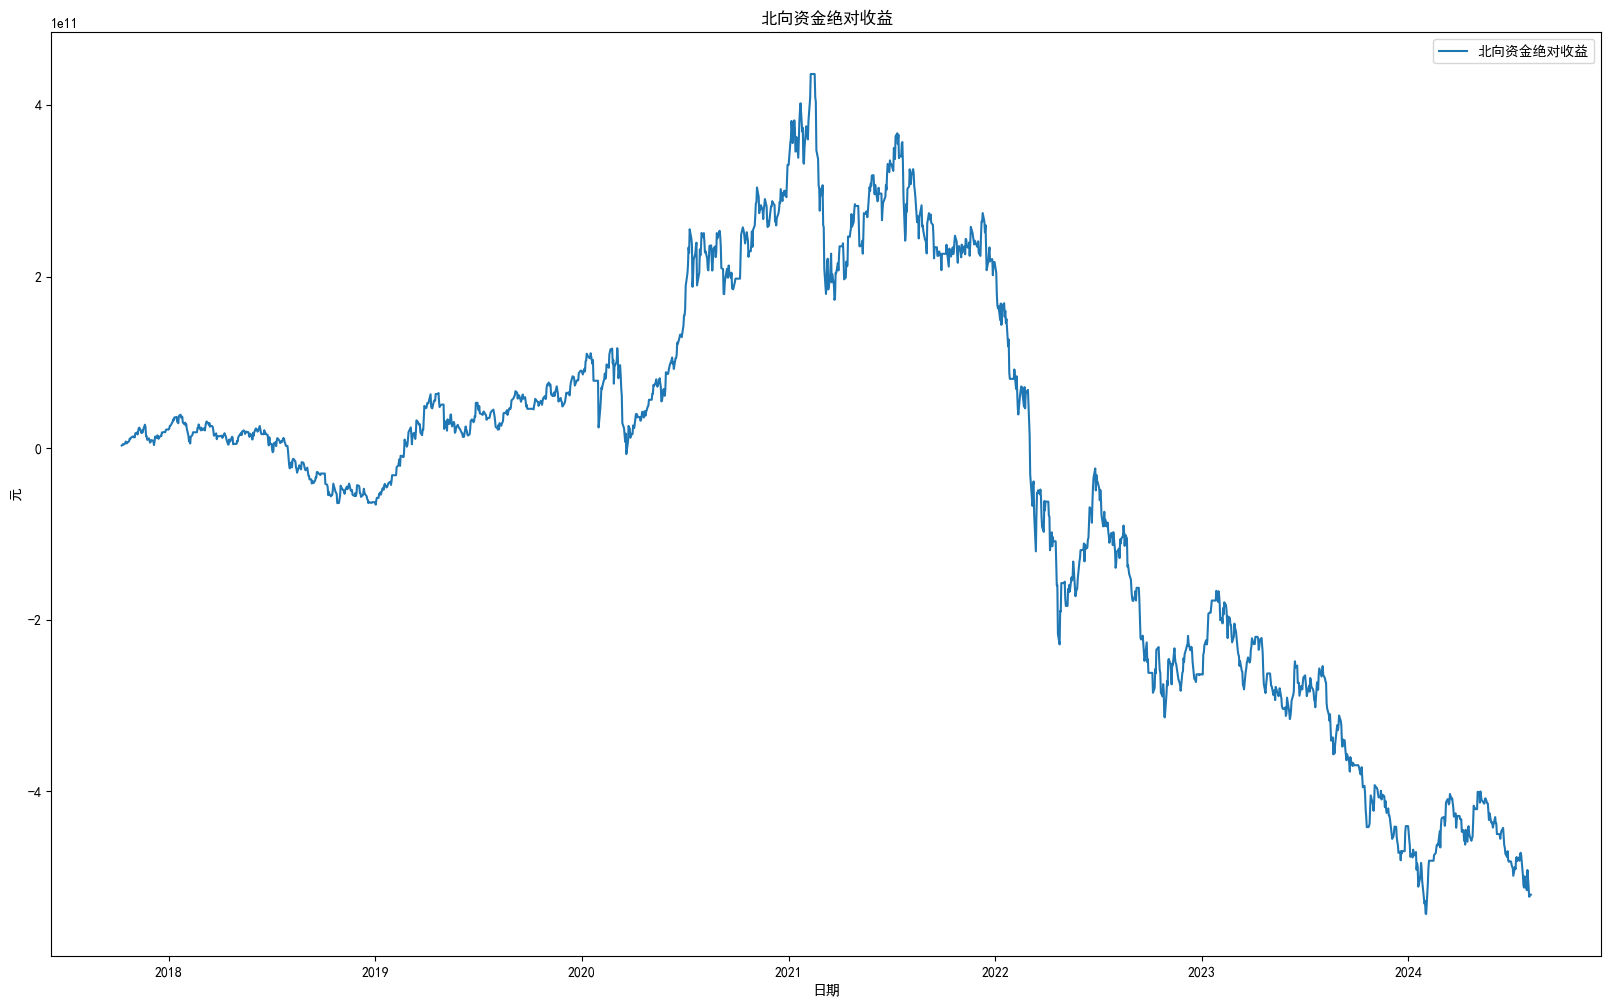
\includegraphics[width=1.15\textwidth]{../Figure/北向绝对收益.png}}
    \caption{北向资金累计绝对收益走势估计（未扣除交易费用）}
    \label{fig:北向累计绝对收益}
    \vspace{0.5em}
    \begin{minipage}{0.95\textwidth}
        \small\textit{注：横轴为交易日期，纵轴为以人民币计价的累计绝对收益金额。收益测算基于每日收盘持仓与次日收盘价变动的乘积累加，未扣除印花税、佣金等交易摩擦成本。}
    \end{minipage}
\end{figure}

值得注意的是，实证结果表明北向资金在样本期间内并未获得显著为正的绝对收益，其累计收益曲线在零值附近上下波动，未呈现出持续向上的趋势。当然，这一基准估计存在两方面的技术局限性：第一，该估计未扣除因调仓操作而产生的交易费用（包括印花税、券商佣金、过户费以及沪深港通特有的结算费用等），这将导致对北向资金实际收益的系统性高估；第二，受限于公开数据的披露频率，我们仅能获取每个交易日收盘时点的持仓明细，从而在方法论上隐含了"北向资金在日内不进行调仓操作、仅通过收盘集合竞价阶段调整持仓"的简化假设——这可能会系统性地低估北向资金通过日内高频交易所获取的价差收益。对上述现象更为合理的经济学解释是：投资者若仅简单地在每个交易日收盘后复制北向资金的最新持仓进行静态配置，而不考虑北向资金的动态调仓信号，则难以获得统计显著为正的绝对回报。换言之，北向资金的"聪明"之处并非体现在其持仓组合的静态配置上，而可能体现在其动态调仓的择时与选股决策中。

然而，当我们将分析视角从静态持仓的绝对收益转向北向资金通过主动交易（即动态调仓）所获取的相对收益时，结论截然不同。具体而言，我们在每个交易日 $t$ 的横截面上，计算北向资金在各沪深港通标的股票上的净流入金额 $\Delta w_{it}$（即当日买入金额减去卖出金额）与该股票在 $t+1$ 日收益率 $r_{i,t+1}$ 的乘积之和 $\sum_{i} \Delta w_{it} \cdot r_{i,t+1}$，以此作为该横截面下北向资金因主动交易行为而产生的相对收益。此处的"相对收益"在经济含义上定义为：以上一交易日收盘时点的静态持仓所能获取的绝对收益为基准（benchmark），北向资金通过当日主动调仓操作所创造的增量价值（incremental value）。将时间序列上每个横截面的相对收益进行逐步累加，即可得到图\ref{fig:北向累计相对收益}所示的累计主动交易收益曲线。

\begin{figure}[htbp]
    \centering
    \makebox[\textwidth][c]{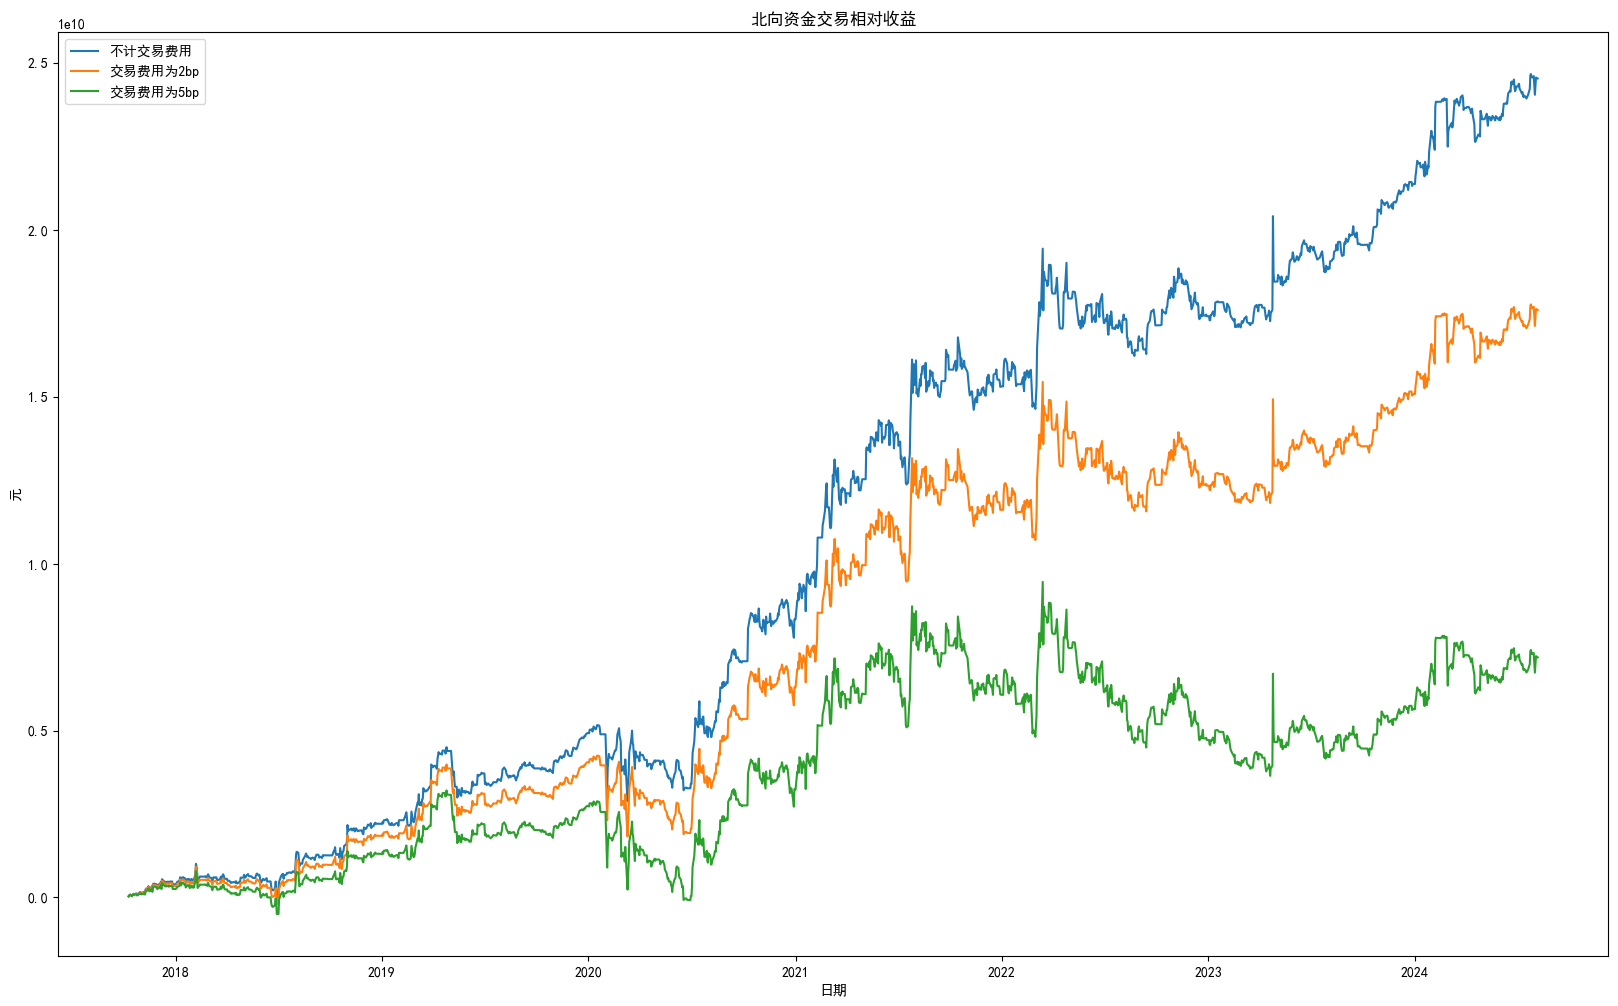
\includegraphics[width=1.15\textwidth]{../Figure/北向交易相对收益.png}}
    \caption{北向资金主动交易累积相对收益（多费率情景测试）}
    \label{fig:北向累计相对收益}
    \vspace{0.5em}
    \begin{minipage}{0.95\textwidth}
        \small\textit{注：蓝线为不考虑交易成本时的累积相对收益；黄线和绿线分别为双边交易费率设定为万分之二（2 bps）和万分之五（5 bps）时的累积相对收益。三条曲线均呈现稳健的上升趋势。}
    \end{minipage}
\end{figure}

图\ref{fig:北向累计相对收益}中，蓝色实线代表在完全不考虑交易摩擦成本时，北向资金每日净买入操作所产生的累积相对收益。考虑到实际交易中投资者需支付印花税（目前为卖出时单边征收千分之一）、券商佣金（通常为万分之二至万分之三）以及其他结算费用等摩擦成本，我们进一步进行了多情景稳健性测试：黄色虚线和绿色点划线分别代表在双边交易费率假设为万分之二（2 basis points）和万分之五（5 basis points）两种较为保守的成本设定下的累积收益表现。正如前文所述，由于北向资金的日内调仓行为无法被收盘时点的持仓快照完整捕捉，图中展示的收益曲线本质上是对北向资金真实相对收益的一个保守下限估计。即便在如此保守的估计框架下，北向资金通过主动调仓操作所获取的相对收益依然呈现出显著且高度稳健的上升趋势，三条收益曲线在整个样本期间内均保持正增长态势，未出现长期回撤。

尽管上述累积收益曲线作为描述性统计工具具有直观清晰的优势，但为了更加严谨地从统计推断角度验证北向资金超额收益的显著性，我们引入了基于假设检验框架的正式统计方法。核心思路是在每个交易日的横截面上，度量北向资金对各标的股票的净流入量与其未来一日回报率之间的截面相关程度，并检验该相关度量在时间序列维度上的均值是否统计显著大于零。为此，我们假设这种截面相关度量在不同交易日之间服从同分布（但允许存在时序自相关），并据此构建单侧 t 检验。本文所采用的修正截面相关系数（Modified Cross-Sectional Correlation Coefficient）度量指标定义如下：

\begin{equation}
    \widetilde{Corr}_t = \frac{\sum\limits_{i=1}^n X_{it}Y_{it}}{\sqrt{\sum\limits_{i=1}^n X_{it}^2}\sqrt{\sum\limits_{i=1}^n Y_{it}^2}}
    \label{eq:tilde_coef}
\end{equation}

其中，$\widetilde{Corr}_t$ 表示在第 $t$ 个交易日的横截面上，北向资金净流入序列与未来一日股票回报序列之间的修正相关系数，其取值范围为 $[-1, 1]$；$X_{it}$ 表示在交易日 $t$ 的横截面上北向资金对第 $i$ 只标的股票的净流入金额（以人民币元计），正值代表净买入，负值代表净卖出；$Y_{it}$ 表示第 $i$ 只标的股票在 $t+1$ 日的收盘至收盘（Close-to-Close）回报率；$n$ 表示交易日 $t$ 横截面上沪深港通标的股票的总数。

式\ref{eq:tilde_coef}本质上是对传统皮尔逊相关系数（Pearson Correlation Coefficient）的一种特定修正。传统皮尔逊相关系数在计算横截面相关性时，会分别对序列 $\{X_{it}\}_{i\in I}$ 和 $\{Y_{it}\}_{i \in I}$ 进行去均值化处理（demeaning），即先减去各自的横截面均值 $\bar{X}_t = \frac{1}{n}\sum_{i}X_{it}$ 和 $\bar{Y}_t = \frac{1}{n}\sum_{i}Y_{it}$，再计算标准化后的协方差。然而，在时间序列维度上，两组截面均值序列 $\{\bar{X}_t\}_{t \in T}$（反映北向资金对市场整体的净流入方向）与 $\{\bar{Y}_t\}_{t \in T}$（反映市场整体的涨跌方向）往往存在非零的正相关关系。而这种宏观层面的正相关性恰恰是择时收益（market timing return）的重要来源——当北向资金整体净流入增加时，若次日市场整体上涨，则说明北向资金具有市场择时能力。式\ref{eq:tilde_coef}的修正逻辑在于强制将两组样本的截面均值设定为零（即省略去均值化步骤），从而使得该指标能够同时衡量两种收益来源：横截面上偏离均值配置的"选股收益"（stock selection return）以及时间序列上顺应市场方向的"择时收益"（market timing return）。

我们建立如下单侧假设检验：原假设 $H_0: E(\widetilde{Corr}_t) \leq 0$，即北向资金的净流入方向与次日股票回报之间不存在正向关联（北向资金不具备预测能力）；备择假设 $H_1: E(\widetilde{Corr}_t) > 0$，即北向资金的净流入方向与次日股票回报之间存在显著的正向关联（北向资金具备统计显著的预测能力）。经计算，各个交易日横截面上 $\widetilde{Corr}_t$ 的经验分布情况如图\ref{fig:corr}所示。

\begin{figure}[htbp]
    \centering
    \makebox[\textwidth][c]{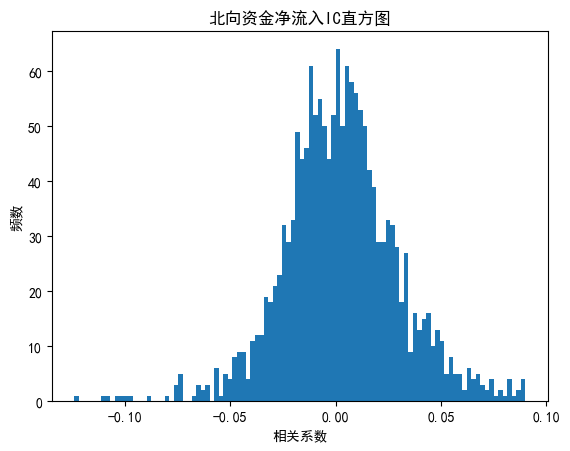
\includegraphics[width=1.15\textwidth]{../Figure/IC直方图.png}}
    \caption{北向资金净流入与次日收益率修正相关系数（$\widetilde{Corr}_t$）分布直方图}
    \label{fig:corr}
    \vspace{0.5em}
    \begin{minipage}{0.95\textwidth}
        \small\textit{注：图中共包含1,560个有效样本点，每个样本点代表一个交易日内北向资金在沪深港通全部标的股票横截面上的净流入金额与各标的股票次日收盘回报率之间的修正相关系数 $\widetilde{Corr}_t$。分布整体呈近似正态，均值略大于零，表明北向资金净流入与次日回报之间存在系统性的正向关联。}
    \end{minipage}
\end{figure}

考虑到修正相关系数的时间序列 $\{\widetilde{Corr}_t\}_{t=1}^{T}$ 可能存在显著的低阶自相关性（autocorrelation）与条件异方差性（conditional heteroskedasticity），传统的 OLS 标准误可能严重低估真实的抽样波动性，从而导致 t 统计量的虚高和过度拒绝原假设。为克服这一问题，我们采用 Newey-West（1987）提出的异方差自相关一致（HAC, Heteroskedasticity and Autocorrelation Consistent）标准误对均值进行显著性测试。在操作上，这等价于在 HAC 协方差矩阵下将修正相关系数序列 $\{\widetilde{Corr}_t\}$ 对常数项进行最小二乘回归，即估计模型 $\widetilde{Corr}_t = \alpha + \epsilon_t$，并检验截距项 $\alpha$ 是否显著大于零。回归结果如表\ref{tab:ols_results_hac}所示：

\begin{table}[htbp]
\centering
\caption{修正相关系数常数项回归结果（Newey-West HAC 检验）}
\label{tab:ols_results_hac}
\begin{threeparttable}
\small
\setlength{\tabcolsep}{6pt}
\renewcommand{\arraystretch}{1.15}

%%% ---- 第一部分：模型概要 ---- %%%
\begin{tabular}{@{}ll@{\hskip 24pt}ll@{}}
\toprule
\textbf{统计指标} & \textbf{数值} & \textbf{拟合优度指标} & \textbf{数值} \\
\midrule
Dep.\ Variable    & $\widetilde{Corr}_t$ & R-squared          & $-0.000$ \\
Model             & OLS                  & Adj.\ R-squared    & $-0.000$ \\
Method            & Least Squares        & F-statistic        & NaN      \\
Date              & 2026-03-01           & Prob (F-statistic) & NaN      \\
Time              & 16:59:23             & Log-Likelihood     & 3988.9   \\
No.\ Observations & 1\,780              & AIC                & $-7\,976$\\
Df Residuals      & 1\,779              & BIC                & $-7\,970$\\
Df Model          & 0                    &                    &          \\
Covariance Type   & HAC                  &                    &          \\
\bottomrule
\end{tabular}

\vspace{6pt}

%%% ---- 第二部分：回归系数表 ---- %%%
\begin{tabular}{@{}lcccc@{}}
\toprule
\textbf{变量}
  & \textbf{系数}
  & \textbf{标准误}
  & \textbf{$z$统计量\;/\;$P>|z|$}
  & \textbf{95\%置信区间} \\
\midrule
常数项\;$\hat{\alpha}$
  & $0.0021^{***}$
  & 0.001
  & 3.82\;/\;0.000
  & $[0.001,\; 0.003]$ \\
\bottomrule
\end{tabular}

\vspace{6pt}

%%% ---- 第三部分：模型诊断检验 ---- %%%
\begin{tabular}{@{}ll@{\hskip 24pt}ll@{}}
\toprule
\textbf{诊断指标} & \textbf{数值} & \textbf{检验指标} & \textbf{数值} \\
\midrule
Omnibus        & 83.586  & Durbin-Watson      & 2.128        \\
Prob(Omnibus)  & 0.000   & Jarque-Bera (JB)   & 283.357      \\
Skew           & 0.005   & Prob(JB)           & $2.95\times10^{-62}$ \\
Kurtosis       & 4.955   & Cond.\ No.         & 1.00         \\
\bottomrule
\end{tabular}

\begin{tablenotes}\footnotesize
\item[\dag] 注：***、**、*分别表示在1\%、5\%、10\%的显著性水平上统计显著。
标准误采用 Newey-West 异方差自相关一致（HAC）估计量，
滞后阶数依据 $\lfloor 4(T/100)^{2/9} \rfloor$ 自动选取，
未使用有限样本校正。
因变量为每日横截面修正相关系数 $\widetilde{Corr}_t$，
共1\,780个交易日观测值。
R-squared 为负值（$-0.000$）系仅含常数项回归的数值精度所致，实质等于零。
Durbin-Watson 统计量为2.128，接近理论无自相关值2，
表明 HAC 校正后残差的低阶自相关已被充分考虑。
Jarque-Bera 检验拒绝了正态性假设（JB $= 283.357$, $p \approx 0$），
结合峰度值4.955表明分布呈尖峰厚尾特征，
进一步验证了采用 HAC 稳健标准误的必要性。
\end{tablenotes}

\end{threeparttable}
\end{table}

回归结果显示，常数项估计值 $\hat{\alpha} = 0.0021$，对应的 Newey-West 稳健 t 统计量为 3.82，远超 1\% 显著性水平对应的临界值2.326（单侧检验临界值为 2.576），p 值趋近于零。这一严谨的假设检验结果从统计推断角度强有力地证实：北向资金通过主动交易（动态调仓）所产生的相对收益是高度显著且稳健的，即北向资金的净流入方向能够系统性地预测标的股票的短期回报，支持了"聪明钱"假说。从经济意义上看，$\hat{\alpha} = 0.0021$ 意味着北向资金净流入与次日回报之间的平均截面相关系数约为千分之二，虽然绝对值不大，但在高维横截面和高频时间序列的复合效应下，足以产生图\ref{fig:北向累计相对收益}所展示的可观累积收益。

\subsubsection{北向资金收益来源分解}
\label{subsec:return_decomposition}

\textit{注：自本小节起至第4节结束，除特别说明外，文中提及的"北向资金收益"均特指第\ref{sec:return_ability}小节中定义的"北向资金主动交易相对收益"（即以前一交易日收盘静态持仓收益为基准，北向资金通过当日动态调仓所创造的增量价值），而非绝对持仓收益。}

\vspace{0.5em}

本小节的研究旨在深入剖析北向资金超额收益的内在来源结构。一般而言，投资者获取超额回报的途径可归纳为两种本质上正交的维度：第一种是\textbf{选股能力}（stock selection ability），即在同一时间截面上识别出哪些个股更可能获得高于截面均值的相对回报，通过在横截面上偏离等权或市值加权基准配置来获取超额收益；第二种是\textbf{择时能力}（market timing ability），即在时间序列上判断市场整体的涨跌方向，在预期市场上涨时增加总体仓位敞口（净买入），在预期市场下跌时降低总体仓位敞口（净卖出），从而通过顺应市场趋势获取超额收益。我们将第一种途径产生的收益称为\textbf{选股收益}（Cross-Sectional PnL, CsPnl），将第二种途径产生的收益称为\textbf{择时收益}（Time-Series PnL, TsPnl）。

在本小节中，我们需要定量地确定北向资金所获取的超额收益中，选股收益与择时收益各自的贡献比例。这一分解不仅有助于我们从更微观的层面理解北向资金信息优势的具体表现形式——究竟是源于对公司基本面差异的深度研究（选股），还是源于对宏观经济走势和市场情绪变化的敏锐感知（择时）——还能为我们在第5节构建基于北向资金信号的量化交易策略时提供明确的方向指引，使策略设计能够有针对性地侧重于贡献度更高的收益来源。

在第\ref{sec:return_ability}小节中，我们引入了修正相关系数指标（式\ref{eq:tilde_coef}）来度量北向资金净流入与未来收益率之间的截面相关程度。该指标之所以不同于传统的皮尔逊相关系数（Pearson Correlation），本质原因在于：传统皮尔逊相关系数在计算前会对两组变量分别进行截面去均值化处理，这一操作在消除截面均值信息的同时，也完全剔除了择时收益的贡献，使其仅能衡量选股收益。而式\ref{eq:tilde_coef}通过省略去均值化步骤，使得该指标能够同时涵盖选股与择时两个维度的收益信息。基于这一观察，我们可以采用一种类似于方差分解（variance decomposition）的方法，将北向资金的总收益在数学上严格分解为选股收益与择时收益两个正交分量。

具体地，设 $\alpha_{i,t}$ 为股票 $i$ 在交易日 $t$ 的北向资金净持仓变化金额（即净流入金额，正值代表净买入，负值代表净卖出）；$r_{i,t+1}$ 为股票 $i$ 在交易日 $t+1$ 的收盘至收盘（Close-to-Close）回报率；$n_t$ 为交易日 $t$ 横截面上沪深港通标的股票总数。我们定义如下三个收益度量：

\begin{equation}
    \text{TotalPnl} = \sum_{t} \sum_{i=1}^{n_t} \alpha_{i,t} \cdot r_{i,t+1}
    \label{eq:total_pnl}
\end{equation}

\begin{equation}
    \text{CsPnl} = \sum_{t} \sum_{i=1}^{n_t} \left(\alpha_{i,t} - \bar{\alpha}_t\right) \cdot \left(r_{i,t+1} - \bar{r}_{t+1}\right), \quad \text{其中} \; \bar{\alpha}_t = \frac{1}{n_t}\sum_{i=1}^{n_t}\alpha_{i,t}, \; \bar{r}_{t+1} = \frac{1}{n_t}\sum_{i=1}^{n_t}r_{i,t+1}
    \label{eq:cs_pnl}
\end{equation}

\begin{equation}
    \text{TsPnl} = \text{TotalPnl} - \text{CsPnl}
    \label{eq:ts_pnl}
\end{equation}

其中，式\ref{eq:total_pnl}的总收益（TotalPnl）等于所有交易日和所有标的股票上北向资金净流入金额与次日回报率乘积的双重求和，即北向资金主动交易创造的全部增量价值。式\ref{eq:cs_pnl}的选股收益（CsPnl）在每个交易日的横截面上，先将净流入序列和回报率序列分别进行去均值化处理（减去各自的截面均值 $\bar{\alpha}_t$ 和 $\bar{r}_{t+1}$），再计算去均值后的乘积之和。这一处理去除了北向资金整体净流入方向与市场整体涨跌方向之间的协变信息，仅保留了北向资金在个股之间差异化配置所产生的收益。式\ref{eq:ts_pnl}将择时收益（TsPnl）定义为总收益与选股收益之差，其经济含义是北向资金通过整体仓位敞口的择时调整（即截面均值层面的净流入方向与市场整体涨跌方向的协变）所获取的收益。

图\ref{fig:revenue_compo}展示了基于上述分解方法对北向资金累计主动交易收益的拆解结果。具体而言，我们将图\ref{fig:北向累计相对收益}中蓝色实线所代表的未扣费累计相对收益，按照式\ref{eq:cs_pnl}和式\ref{eq:ts_pnl}的定义分解为选股收益和择时收益两个分量，并在时间序列上分别绘制其累计曲线。

\begin{figure}[htbp]
    \centering
    \makebox[\textwidth][c]{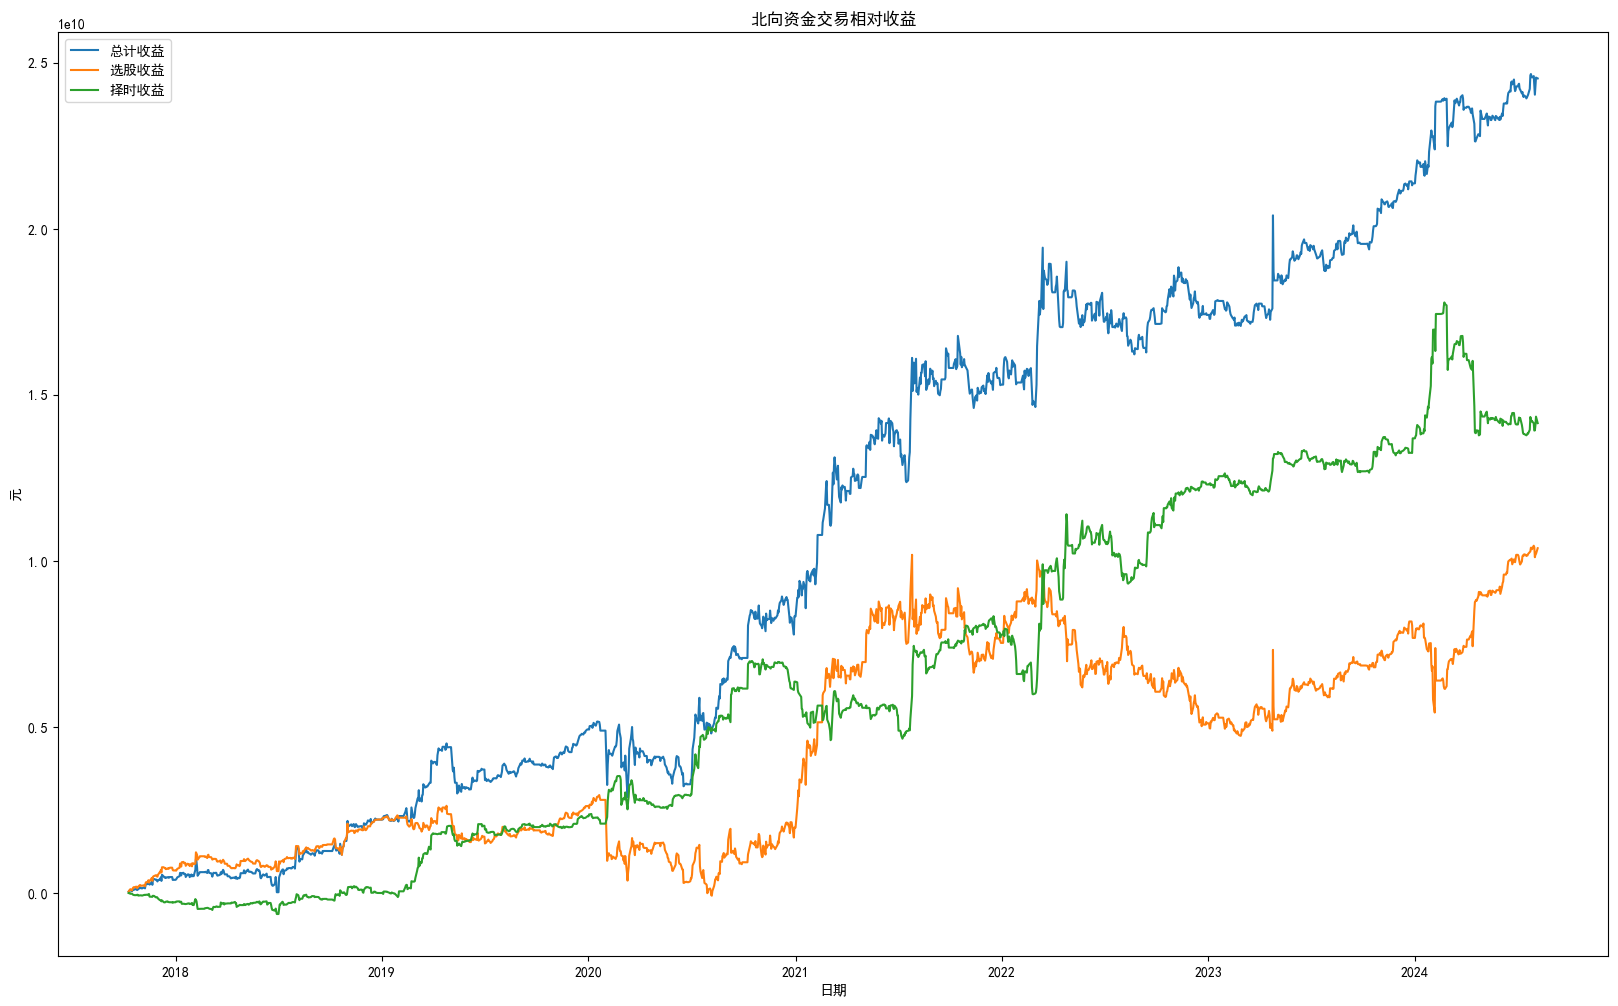
\includegraphics[width=1.15\textwidth]{../Figure/收益分解.png}}
    \caption{北向资金主动交易累计收益的选股—择时分解}
    \label{fig:revenue_compo}
    \vspace{0.5em}
    \begin{minipage}{0.95\textwidth}
        \small\textit{注：图中展示了北向资金累计主动交易收益（总收益）及其分解为选股收益（CsPnl）和择时收益（TsPnl）两个分量后的累计曲线。横轴为交易日期，纵轴为以人民币计价的累计收益金额。总收益等于选股收益与择时收益之和。}
    \end{minipage}
\end{figure}

从图\ref{fig:revenue_compo}中可以观察到，北向资金的累计主动交易收益中，择时收益的累计曲线在样本期间内的终值高于选股收益，表明择时能力是北向资金超额收益的主要来源。为了更精确地量化两种收益来源的相对贡献，我们将选股收益与择时收益的累计金额、年化夏普比率（Annualized Sharpe Ratio）以及对总收益的贡献度汇总于表\ref{tab:return_decomposition}中。

\begin{table}[htbp]
    \centering
    \caption{北向资金主动交易收益的选股—择时分解统计}
    \label{tab:return_decomposition}
    \makebox[\textwidth][c]{%
    \begin{tabular}{lccc}
        \toprule
        \textbf{收益类型} & \textbf{累计收益金额（人民币元）} & \textbf{年化夏普比率} & \textbf{贡献度} \\
        \midrule
        选股收益（CsPnl） & $1.039 \times 10^{10}$ & 1.04 & 42.34\% \\
        择时收益（TsPnl） & $1.415 \times 10^{10}$ & 0.82 & 57.66\% \\
        \midrule
        总收益（TotalPnl） & $2.454 \times 10^{10}$ & 1.38 & --- \\
        \bottomrule
    \end{tabular}%
    }
    \vspace{0.5em}
    \begin{minipage}{0.95\textwidth}
        \footnotesize\textit{注：年化夏普比率的计算方法为日度平均回报率除以日度回报率标准差，再乘以 $\sqrt{252}$ 进行年化。贡献度定义为各分量累计收益金额占总累计收益金额的百分比。累计收益金额未扣除交易费用。}
    \end{minipage}
\end{table}

表\ref{tab:return_decomposition}揭示了一个值得深入讨论的现象：尽管择时收益的累计金额（$1.415 \times 10^{10}$ 元，贡献度 57.66\%）显著高于选股收益（$1.039 \times 10^{10}$ 元，贡献度 42.34\%），但选股收益的年化夏普比率（1.04）反而高于择时收益（0.82）。这意味着从风险调整后的收益效率角度衡量，选股收益实际上比择时收益更为稳定和高效。造成"低夏普比率但高累计金额"这一看似矛盾现象的可能解释是：择时收益的分布呈现出较强的右偏特征——即择时收益在绝大多数交易日表现平淡，但在少数特定交易日（如市场出现大幅单边行情、北向资金大规模净流入或净流出的交易日）产生远超均值的极端正收益。这些集中出现的大幅正收益显著推高了累计金额，但同时也增大了日度回报率的波动性（标准差），从而降低了夏普比率。相比之下，选股收益在时间序列上的分布更为均匀，日间波动较小，因此虽然累计金额略低，但风险调整后的表现更为优异。

通过本小节的收益来源分解分析，我们获得了两个关键发现：第一，北向资金的超额收益同时来源于选股能力和择时能力，且择时收益在绝对金额上贡献更大（57.66\%）；第二，选股收益虽然绝对贡献较小，但具有更高的夏普比率（1.04 vs. 0.82），表现出更强的稳定性。这些发现对第5节的量化策略构建具有重要的指导意义：若希望在第\ref{sec:return_ability}小节所展示的基础收益之上进一步提升策略表现，应当重点挖掘北向资金日度持仓净变化在时间序列维度上的预测性规律（即择时信号），因为这一维度不仅贡献了更大比例的超额收益，且其潜在的可预测性尚未被充分开发。

\subsubsection{北向资金交易模式分析}
\label{sec:trading_pattern}

在前一小节（第\ref{subsec:return_decomposition}小节）的收益分解分析中，我们发现北向资金超额收益的主要来源是择时收益而非选股收益。这一发现引出了一个重要的推论：北向资金的交易模式可能更接近于高换手率的\textbf{对冲基金}（hedge fund）模式，而非低换手率的\textbf{共同基金}（mutual fund）模式。其背后的经济逻辑在于：作为长期持有者和价值投资者的共同基金，其获利的核心途径是在横截面上通过深度基本面研究识别被低估的标的，从而在长期持有中获取选股收益——这种策略并不要求频繁的仓位调整。然而，若一个投资者的超额收益主要来源于择时能力，即通过准确判断市场短期涨跌方向并据此调整总体仓位敞口来获利，那么这类投资者的换手率很可能显著高于市场平均水平——因为实现择时收益在逻辑上要求投资者根据市场信号频繁地增减仓位，采取更为活跃的交易策略。

上述推论与以往文献和市场实务中的主流认知形成了鲜明反差。既有研究和市场评论通常将北向资金默认为以长线配置和价值投资为主导的机构投资者群体，并在此预设基础上展开对北向资金交易行为的分析或基于北向资金信号的量化策略设计。然而，如果这一预设与事实不符，则相关研究结论和策略逻辑的可靠性将受到根本性的挑战。因此，本小节旨在通过实证检验验证以下假说：北向资金的交易模式呈现出高换手率、广泛选股的"对冲基金模式"特征，而非低换手率、集中持有的"价值投资模式"。

为检验上述假说，我们首先需要构建适用于北向资金的换手率度量指标。在一般的股票市场交易中，对于每一笔成交，买方的买入量恒等于卖方的卖出量，因此在任何给定时间区间内，某只股票的总买入金额与总卖出金额总是相等的。基于这一对称性，传统的换手率通常定义为：

\begin{equation}
    \text{Turnover}_i := \frac{\text{TransactionValue}_i}{\text{MarketValue}_i}
    \label{eq:turnover}
\end{equation}

\noindent 即资产 $i$ 在给定时间区间内的总成交金额除以资产 $i$ 的总流通市值（取区间均值）。

然而，值得注意的是，北向资金作为A股市场中的一个特定投资者群体，其买入和卖出操作的对手方均可以是内地本土投资者（包括境内机构和个人投资者）。这意味着在任何给定交易日内，北向资金在某只标的股票上的买入金额与卖出金额可能并不相等\footnote{例如，某一交易日内北向资金可能仅买入某只股票1亿元而未进行任何卖出操作，与此同时，内地本土投资者作为对手方卖出了相应的1亿元股票但可能并未通过沪深港通渠道买入。这种非对称性在北向资金呈现单边净流入或净流出态势时尤为显著。}。因此，直接套用式\ref{eq:turnover}的传统换手率计算方式将会产生偏误。为此，我们对换手率指标进行如下修正，定义北向资金的\textbf{交易率}（Trading Intensity）指标：

\begin{equation}
    T_i := \frac{\text{BuyValue}_i + \text{SellValue}_i}{2 \times \text{PositionValue}_i}
    \label{eq:my_turnover}
\end{equation}

\noindent 即资产 $i$ 在给定时间区间内北向资金的总买入金额与总卖出金额之和，除以北向资金在该资产上的持仓市值（取区间均值）的两倍。分母中乘以2的原因是为了与传统换手率的口径保持一致——在传统定义中，成交金额已经同时包含了买方的买入和卖方的卖出（双边计算），而此处我们将买入和卖出分别加总后需除以2以转换为等价的单边口径。

事实上，对于全市场所有交易者的集合体而言，由于买卖双方的成交量恒等，式\ref{eq:my_turnover}所定义的交易率在数学上与式\ref{eq:turnover}的传统换手率完全等价。这一等价性使得我们能够在同一度量标准下，直接对比北向资金与A股全市场的交易活跃程度。对比结果如图\ref{fig:turnover_1}所示。

\begin{figure}[htbp]
    \centering
    \makebox[\textwidth][c]{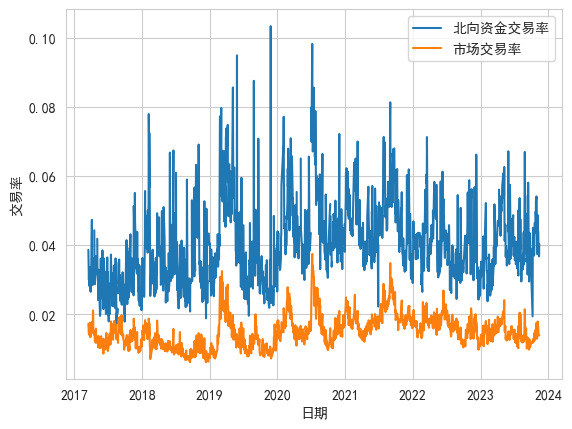
\includegraphics[width=1.15\textwidth]{../Figure/turnover_1.png}}
    \caption{北向资金交易率与A股全市场换手率的对比（未经调整的原始数据）}
    \label{fig:turnover_1}
    \vspace{0.5em}
    \begin{minipage}{0.95\textwidth}
        \small\textit{注：图中分别展示了北向资金依据式\ref{eq:my_turnover}计算的交易率，与A股全市场依据式\ref{eq:turnover}计算的传统换手率。两个指标在全市场层面数学等价，因此具有直接可比性。横轴为交易日期，纵轴为日度换手率/交易率（单位：\%）。}
    \end{minipage}
\end{figure}

图\ref{fig:turnover_1}的初步结果确实令人惊讶：北向资金的交易率远高于A股全市场的整体换手率，差距之大达到了异常的程度。然而，深入思考A股市场的微观结构和股东持股特征后，我们发现上述原始对比存在显著的偏误，其结论需要谨慎解读。偏误的主要来源在于A股上市公司特殊的\textbf{股东结构}：A股上市公司中，持股量排名前列的大股东（通常为创始人家族、国有资本、战略投资者等）所持有的股份虽然在统计口径上被计入流通市值，但这些股份在实际交易中的流动性极低——大股东出于控制权维护、锁定期约束、减持规则限制等原因，极少参与二级市场的日常交易。这一特征与成熟市场（如美国市场）中大股东主要为共同基金、养老金等机构投资者且持仓流动性较高的情况形成鲜明对比。因此，以包含大量低流动性大股东持仓的全市场流通市值作为分母，将导致全市场换手率被严重低估，从而夸大了北向资金与全市场之间的换手率差距。

为修正上述偏误，我们需要将全市场换手率调整为特定投资者群体（如活跃机构投资者或个人投资者）的实际换手率。具体的调整方法如下：若已知A股成交金额中某类投资者（如机构投资者或个人投资者）的交易贡献占比为 $a$，且该类投资者的持仓市值占A股总流通市值的比例为 $b$，则该类投资者的调整换手率可表示为：

\begin{equation}
    \text{AdjTurnover}_i := \frac{\text{TransactionValue}_i \times a}{\text{MarketValue}_i \times b}
    \label{eq:adjturnover}
\end{equation}

\noindent 式\ref{eq:adjturnover}的经济含义是：分子仅保留该类投资者贡献的成交金额部分，分母仅保留该类投资者实际持有的市值部分，从而得到该类投资者群体的"真实"换手率。

为实施上述调整，我们利用表\ref{tab:holding}所示的上海证券交易所公布的投资者结构数据（由CEIC数据库收集整理）来估算不同类型投资者的交易贡献比例和持股比例。

\begin{table}[htbp]
    \centering
    \caption{上海证券交易所各类投资者交易占比与持股占比（年度数据）}
    \label{tab:holding}
    \makebox[\textwidth][c]{%
    \begin{tabular}{ccccc}
        \toprule
        \textbf{年份} & \textbf{机构交易占比（\%）} & \textbf{个人交易占比（\%）} & \textbf{机构持股占比（\%）} & \textbf{个人持股占比（\%）} \\
        \midrule
        2007 & 10.37 & 86.01 & 33.74 & 48.29 \\
        2008 & 12.83 & 83.21 & 26.24 & 42.23 \\
        2009 & 10.82 & 85.36 & 16.95 & 26.47 \\
        2010 & 12.98 & 84.59 & 15.88 & 23.13 \\
        2011 & 14.39 & 83.52 & 15.21 & 20.47 \\
        2012 & 17.12 & 80.78 & 16.92 & 19.74 \\
        2013 & 15.30 & 82.24 & 14.58 & 21.78 \\
        2014 & 11.60 & 85.19 & 14.65 & 23.51 \\
        2015 & 10.47 & 86.91 & 14.49 & 25.18 \\
        2016 & 12.21 & 85.62 & 15.58 & 23.70 \\
        2017 & 14.76 & 82.01 & 16.13 & 21.17 \\
        2018 & ---   & ---   & 13.92 & 19.62 \\
        2019 & ---   & ---   & 15.74 & 20.59 \\
        2020 & ---   & ---   & 17.77 & 22.93 \\
        2021 & ---   & ---   & 19.14 & 24.48 \\
        2022 & ---   & ---   & 21.69 & 23.19 \\
        \bottomrule
    \end{tabular}%
    }
    \vspace{0.5em}
    \begin{minipage}{0.95\textwidth}
        \footnotesize\textit{注：数据来源为上海证券交易所统计年鉴，由CEIC数据库收集整理。交易占比与持股占比之和不等于100\%，差额部分为未分类的其他投资者类型（如沪股通等跨境资金）。"---"表示相应年份该数据未公布。机构投资者包括证券公司自营、公募基金、私募基金、保险资金、社保基金、QFII等；个人投资者指以自然人名义开户的散户投资者。}
    \end{minipage}
\end{table}

关于表\ref{tab:holding}中数据的使用，需要说明以下几个局限性及我们的处理方式。第一，该数据仅提供年度汇总统计，时间粒度较粗，因此后续基于该数据的换手率调整无法给出精确的逐日定量结果，更多地是为读者提供量级层面的直观参照。第二，该数据的有效时间区间（交易占比数据截至2017年）与我们的北向资金持仓数据覆盖区间（2017年10月9日至2025年）几乎没有重叠，这给直接对比带来了困难。

为解决数据时间区间不匹配的问题，我们需要引入一个关键的稳定性假设：即2017年之后各类投资者的交易习惯（具体定义为某类投资者的换手率与全市场换手率的比值，即"相对换手倍数"）相较于2017年之前没有发生结构性变化。从表\ref{tab:holding}中2012年之后的数据来看\footnote{2012年之前与之后的数据确实存在较为明显的结构性差异，这与2012年前后中国金融市场经历的一系列自由化改革（包括融资融券业务扩容、转融通机制推出、QFII额度大幅扩大等）密切相关。因此我们将2012年之后的数据作为稳定期的参考基准。}，各类投资者的交易占比和持股占比在年度间的波动幅度有限，表明上述稳定性假设在合理范围内是可以接受的。此外，为最大程度保证结论的稳健性，我们在后续调整中将采用保守的参数设定，使得调整后的对比基准\textit{上界}仍然低于北向资金的交易率。

从表\ref{tab:holding}中可以计算各类投资者的"相对换手倍数"（Relative Turnover Multiplier），定义为：
\begin{equation}
    R_k = \frac{\text{TransactionRatio}_k}{\text{HoldingRatio}_k}
    \label{eq:relative_turnover}
\end{equation}

\noindent 其中 $k$ 表示投资者类型（机构或个人），$\text{TransactionRatio}_k$ 为该类投资者的交易占比，$\text{HoldingRatio}_k$ 为其持股占比。计算结果显示：机构投资者的相对换手倍数 $R_{\text{机构}}$ 在0.8至1.1之间波动，表明机构投资者的换手率与其持仓规模大致匹配；而个人投资者的相对换手倍数 $R_{\text{个人}}$ 则高达3.5至4.0，反映出散户交易的高度活跃性远超其持仓占比。

基于上述计算，我们进行两组稳健性对比。在第一组对比中，我们将图\ref{fig:turnover_1}中的全市场换手率乘以1.5倍的调整系数。由于机构投资者的相对换手倍数上限约为1.1，乘以1.5后所得到的调整换手率将\textit{稳健地高于}内地机构投资者的真实换手率，从而构成一个保守的上界基准。在此调整下，北向资金交易率与内地机构投资者调整换手率的对比结果如图\ref{fig:turnover_2}所示。

\begin{figure}[htbp]
    \centering
    \makebox[\textwidth][c]{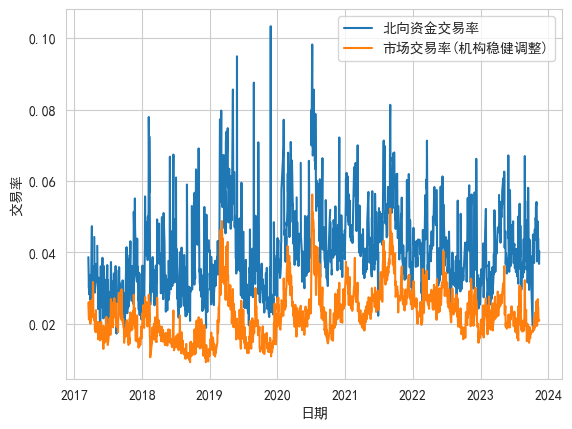
\includegraphics[width=1.15\textwidth]{../Figure/turnover_2.png}}
    \caption{北向资金交易率与内地机构投资者调整换手率的对比（1.5倍稳健调整）}
    \label{fig:turnover_2}
    \vspace{0.5em}
    \begin{minipage}{0.95\textwidth}
        \small\textit{注：橙色线为全市场换手率乘以1.5倍调整系数后的结果，作为内地机构投资者真实换手率的保守上界。蓝色线为北向资金依据式\ref{eq:my_turnover}计算的交易率。}
    \end{minipage}
\end{figure}

在第二组对比中，我们将全市场换手率乘以4倍的调整系数。由于个人投资者的相对换手倍数上限约为4.0，乘以4后所得到的调整换手率将\textit{稳健地高于}内地散户投资者的真实换手率。在此调整下的对比结果如图\ref{fig:turnover_3}所示。

\begin{figure}[htbp]
    \centering
    \makebox[\textwidth][c]{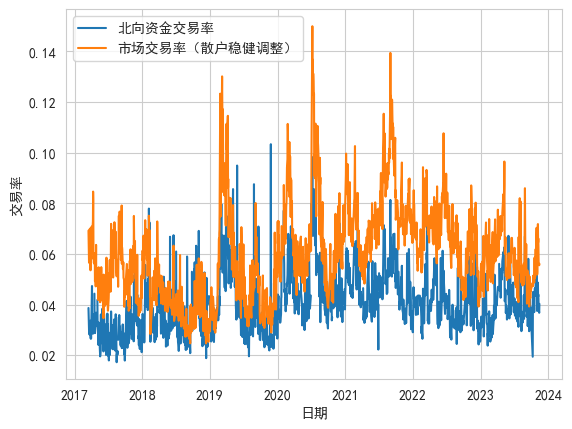
\includegraphics[width=1.15\textwidth]{../Figure/turnover_3.png}}
    \caption{北向资金交易率与内地个人投资者调整换手率的对比（4倍稳健调整）}
    \label{fig:turnover_3}
    \vspace{0.5em}
    \begin{minipage}{0.95\textwidth}
        \small\textit{注：橙色线为全市场换手率乘以4倍调整系数后的结果，作为内地个人投资者（散户）真实换手率的保守上界。蓝色线为北向资金依据式\ref{eq:my_turnover}计算的交易率。}
    \end{minipage}
\end{figure}

从图\ref{fig:turnover_2}和图\ref{fig:turnover_3}中可以得出以下关键观察。第一，即便在采用1.5倍保守上界调整后（图\ref{fig:turnover_2}），北向资金的交易率仍然\textit{远高于}内地机构投资者的换手率上界，两者之间存在显著且持续的差距。这一结果有力地否定了"北向资金为典型的低换手率长线机构投资者"这一传统认知。第二，在采用4倍保守上界调整后（图\ref{fig:turnover_3}），北向资金的交易率与内地散户投资者的换手率上界已十分接近，甚至在部分时间段内超过了后者。考虑到4倍调整系数已是散户相对换手倍数的上界估计，这一结果意味着北向资金的实际交易活跃程度\textit{至少与A股散户投资者相当}，远非传统认知中的"长线价值投资者"形象。

上述令人瞩目的实证发现在相当程度上印证了我们基于收益分解分析所提出的假说：北向资金的交易模式更接近于高换手率、依赖择时和广泛选股的对冲基金模式，而非低换手率、集中持有优质标的的共同基金或价值投资模式。这一发现对于基于北向资金信号的量化策略设计具有重要的方法论启示：有效的策略应当将预测目标锁定在\textbf{短期回报}（如未来1至5个交易日的收益率），并在\textbf{全市场范围}内进行广泛选股，充分利用北向资金在大量标的上的差异化流入信号。相反，若将预测目标设定为长期回报率（如未来数月或数季度的累计收益），或将选股范围局限于沪深300等窄基指数成分股，则可能与北向资金实际的交易模式和信息时效性不匹配，从而难以有效捕捉其蕴含的alpha信号。我们将在下一小节通过对北向资金长短期预测能力的对比检验，为上述策略设计原则提供进一步的实证支撑。

\subsubsection{北向资金对证券长期与短期回报的相对预测能力}
\label{sec:prediction_horizon}

本小节旨在系统性地评估北向资金在不同预测期限（horizon）下对个股回报率的预测能力差异，具体涵盖从一个月（21个交易日）到一年（252个交易日）的多个时间跨度。这一研究具有双重目的：

第一，从量化策略设计的角度，本小节的实证结果将为第\ref{sec:trading_pattern}小节末尾提出的策略设计原则——即应将预测目标锁定在短期回报而非长期趋势——提供直接的补充验证。若北向资金仅在短期预测上具备显著能力，则进一步确认了以短期回报为目标函数的策略设计方向的合理性。

第二，从市场监管与政策分析的角度，本小节的发现为评估北向资金对A股市场定价效率的影响提供了关键的实证基础。若将市场中证券价格的时间序列走势在频域上分解为\textbf{长期趋势分量}（低频成分，反映公司基本面价值的渐进回归）和\textbf{短期波动分量}（高频成分，反映市场情绪、流动性冲击等短期扰动），那么北向资金若要发挥提升市场\textbf{价格发现效率}（price discovery efficiency）的积极作用，其预测能力应当主要体现在对长期趋势分量的准确判断上——即能够识别股价相对于基本面价值的偏离，并通过交易行为推动价格向内在价值回归。然而，第\ref{sec:trading_pattern}小节所揭示的北向资金高换手率特征使我们产生了一个值得警惕的理论猜想：北向资金的信息优势可能主要体现在对短期波动分量的预测上，而对长期基本面趋势则缺乏显著的判断力。若事实确实如此，北向资金不仅无法通过引导价格回归基本面来平抑市场波动、提升定价效率，反而可能因其高频交易行为对短期价格波动形成正反馈效应，从而\textit{加剧}A股市场的短期非理性波动。

\vspace{0.5em}
\noindent\textbf{检验方法}

我们采用如下的多期限截面相关性检验方法。对于给定的时间窗口长度 $n$（以交易日计），在每个交易日 $t$ 的横截面上，计算过去 $n$ 个交易日内各标的股票北向资金累积净流入的移动平均值与未来 $n$ 个交易日内各标的股票累积回报率的移动平均值之间的皮尔逊相关系数，并检验该相关系数在时间序列维度上的均值是否显著大于零。我们选择的时间窗口长度 $n$ 分别为：5个交易日（约1周）、21个交易日（约1个月）、63个交易日（约1个季度）、126个交易日（约半年）和252个交易日（约1年），以涵盖从短期到长期的完整预测期限谱系。

具体地，设 $\text{MA}_n(\text{Inflow})_{i,t}$ 表示股票 $i$ 在交易日 $t$ 上过去 $n$ 个交易日内北向资金日均净流入金额（即 $n$ 阶向后移动平均净流入），$\text{MA}_n(\text{Return})_{i,t}$ 表示股票 $i$ 在交易日 $t$ 上未来 $n$ 个交易日内的日均回报率（即 $n$ 阶向前移动平均回报率）。为确保因变量（未来回报）相对于自变量（历史净流入）的时序先后关系，我们对净流入序列施加 $n$ 阶滞后，即使用 $L_n\text{MA}_n(\text{Inflow})_{i,t} \equiv \text{MA}_n(\text{Inflow})_{i,t-n}$。在此基础上，定义交易日 $t$ 横截面上的截面相关系数为：

\begin{equation}
    \rho_t^{(n)} = \text{Corr}\!\left(\left\{L_n\text{MA}_n(\text{Inflow})_{i,t}\right\}_{i=1}^{N_t},\; \left\{\text{MA}_n(\text{Return})_{i,t}\right\}_{i=1}^{N_t}\right)
    \label{eq:multi_horizon_corr}
\end{equation}

\noindent 其中 $N_t$ 为交易日 $t$ 横截面上可用标的股票总数，$\text{Corr}(\cdot,\cdot)$ 表示标准皮尔逊相关系数。

我们对每个时间窗口长度 $n$ 分别建立如下单侧假设检验：

\begin{equation*}
    H_0^{(n)}:\; E\!\left(\rho_t^{(n)}\right) \leq 0 \qquad \text{vs.} \qquad H_1^{(n)}:\; E\!\left(\rho_t^{(n)}\right) > 0
\end{equation*}

\noindent 即原假设认为北向资金在 $n$ 日预测期限下不具备正向预测能力，备择假设认为北向资金的历史净流入方向与未来回报之间存在显著的正向关联。

\vspace{0.5em}
\noindent\textbf{实证结果}

我们首先针对上述四种较长时间窗口（1个月、1个季度、半年、1年）分别计算截面相关系数序列 $\{\rho_t^{(n)}\}$，所得经验分布的直方图如图\ref{fig:periods}所示。

\begin{figure}[htbp]
    \centering
    \makebox[\textwidth][c]{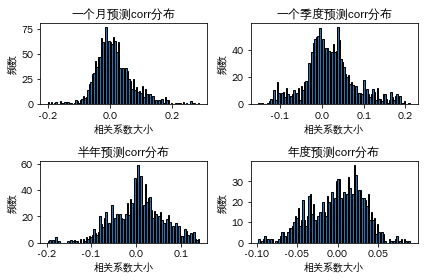
\includegraphics[width=1.15\textwidth]{../Figure/periods.png}}
    \caption{不同预测期限下北向资金净流入与未来回报截面相关系数（$\rho_t^{(n)}$）的经验分布}
    \label{fig:periods}
    \vspace{0.5em}
    \begin{minipage}{0.95\textwidth}
        \small\textit{注：四幅子图分别展示了预测期限 $n$ 为21个交易日（约1个月）、63个交易日（约1个季度）、126个交易日（约半年）和252个交易日（约1年）时，各交易日横截面相关系数 $\rho_t^{(n)}$ 的直方图。每个样本点代表一个交易日 $t$ 上北向资金过去 $n$ 日累积净流入的移动平均值与未来 $n$ 日累积回报移动平均值之间的截面皮尔逊相关系数。}
    \end{minipage}
\end{figure}

从图\ref{fig:periods}中可以初步观察到，在上述四种时间跨度下，截面相关系数 $\rho_t^{(n)}$ 序列的经验分布均大致以零为中心对称分布，未呈现出明显偏离零的均值偏移。这一直观观察提示北向资金在中长期预测期限下的预测能力可能较为有限。为对此进行严格的统计推断，考虑到截面相关系数的时间序列在使用重叠窗口（overlapping windows）计算时会产生显著的高阶自相关结构（移动平均导致的机械自相关），我们采用 Newey-West 异方差自相关一致（HAC）稳健 $t$ 检验对均值的显著性进行判断。检验结果汇总于表\ref{tab:multi_horizon_test}中。

\begin{table}[htbp]
    \centering
    \caption{不同预测期限下北向资金净流入与未来回报截面相关系数的 Newey-West 稳健检验}
    \label{tab:multi_horizon_test}
    \makebox[\textwidth][c]{%
    \begin{tabular}{lcccc}
        \toprule
        \textbf{统计指标} & \textbf{1个月（$n=21$）} & \textbf{1个季度（$n=63$）} & \textbf{半年（$n=126$）} & \textbf{1年（$n=252$）} \\
        \midrule
        相关系数均值 $\bar{\rho}^{(n)}$ & $0.0115^{**}$ & $0.0188^{**}$ & $0.0037$ & $-0.0010$ \\
        Newey-West $t$ 统计量 & 2.16 & 2.69 & 0.53 & $-0.24$ \\
        相关系数为正的交易日占比 & 53.29\% & 60.79\% & 55.49\% & 53.68\% \\
        \bottomrule
    \end{tabular}%
    }
    \vspace{0.5em}
    \begin{minipage}{0.95\textwidth}
        \footnotesize\textit{注：***、**、*分别表示在1\%、5\%、10\%的显著性水平上统计显著（单侧检验）。标准误采用 Newey-West HAC 估计量，滞后阶数依据 $\lfloor 4(T/100)^{2/9} \rfloor$ 自动选取。"相关系数为正的交易日占比"指在全部有效交易日样本中，$\rho_t^{(n)} > 0$ 的交易日所占百分比。}
    \end{minipage}
\end{table}

表\ref{tab:multi_horizon_test}的结果揭示了一个清晰且具有重要经济含义的递减模式。

在\textbf{1个月}（$n=21$）的预测期限下，截面相关系数均值 $\bar{\rho}^{(21)} = 0.0115$，对应的 Newey-West 稳健 $t$ 统计量为 2.16，在 5\% 的显著性水平下拒绝原假设。在\textbf{1个季度}（$n=63$）的预测期限下，$\bar{\rho}^{(63)} = 0.0188$，$t$ 统计量进一步升至 2.69，同样在 5\% 水平下显著。然而，需要特别指出的是，尽管这两个估计在统计意义上达到了显著性门槛，但从\textbf{经济显著性}（economic significance）和\textbf{实务可操作性}的角度审视，其预测力仍然相当有限。

随着预测期限的进一步延长，北向资金的预测能力呈现出单调递减的趋势。在\textbf{半年}（$n=126$）的预测期限下，$\bar{\rho}^{(126)}$ 骤降至 0.0037，对应的 $t$ 统计量仅为 0.53，远低于任何常用显著性水平的临界值，无法拒绝原假设。在\textbf{1年}（$n=252$）的预测期限下，$\bar{\rho}^{(252)}$ 甚至变为负值（$-0.0010$），$t$ 统计量为 $-0.24$，表明在年度尺度上北向资金的历史净流入方向与未来回报之间完全不存在正向预测关系。

将上述多期限检验结果与第\ref{sec:return_ability}小节的日频检验结果（$\bar{\widetilde{Corr}} = 0.0021$，$t = 3.82$，在 1\% 水平下高度显著）进行综合对比，可以勾勒出北向资金预测能力随期限变化的完整图景：北向资金在仅考虑次日回报（$n=1$）时展现出最强且最稳健的预测能力（$t = 3.82$），在短中期（1个月至1个季度）尚保留一定的统计显著性但经济意义有限（$t = 2.16 \sim 2.69$），而在半年及以上的长期预测期限下则完全丧失预测力（$t < 1$）。这一从短期到长期预测能力单调衰减的模式，有力地表明北向资金的信息优势高度集中于\textbf{极短期的价格波动预测}，而非对公司基本面内在价值的长期判断。

上述实证发现与 \textcite{doi:10.1080/1540496X.2015.1011531} 的研究结论相互印证。该研究考察了全球范围内跨国证券投资组合的超额收益实现路径，发现外国机构投资者在东道国（host country）股票市场上获取的超额收益往往在短期内集中实现，而非通过长期持有逐步累积。作者将这一现象称为"短期异质性"（short-horizon heterogeneity），并将其归因于外资投资者在信息获取和处理上的时效性优势——外资机构虽然拥有成熟的投研体系和全球化的信息网络，但其对东道国公司微观基本面的深度理解可能不及本土机构投资者，因此其信息优势更多体现在对全球宏观信号、跨市场联动效应和短期市场微观结构特征的敏锐捕捉上。我们关于北向资金预测能力随期限递减的发现，从中国A股市场的特定场景为这一国际文献的结论提供了新的佐证。

综合本小节的实证结果，我们可以得出以下政策含义层面的推论。北向资金对A股市场的影响可能是\textbf{复杂而双面}的。正如前文的频域分解框架所阐述的，只有当北向资金具备对股价长期趋势（即基本面价值）的准确判断能力时，其交易行为才能发挥引导价格回归内在价值、提升市场定价效率和平抑短期非理性波动的积极功能。然而，现有证据一致表明，北向资金的信息优势高度集中于短期价格波动的预测，而对长期基本面趋势的判断力趋近于零。从理论上分析，这种以短期预测为主导的交易模式可能产生以下负面效应：当北向资金基于短期信号进行高频交易时，其大规模的方向性买卖可能通过\textbf{信息传递效应}（information transmission）和\textbf{流动性冲击效应}（liquidity impact）引发内地投资者的跟风交易（即\textbf{羊群效应}，herding behavior），形成正反馈交易循环，从而\textit{系统性地放大}A股市场的短期波动率，而非起到稳定市场的作用。这一理论推测是否与实际数据相符，将是我们在下一节（第\ref{sec:impact}节）中进行详细实证检验的核心问题。

\subsection{北向资金对A股市场的影响}
\label{sec:impact}

在本节中，我们从两个互补的维度系统性地实证检验北向资金对A股市场的影响效应。

第一个维度聚焦于北向资金对A股股票\textbf{回报率}（即成交额与价格动量）的影响。具体而言，我们运用向量自回归（VAR）模型框架下的格兰杰因果检验（Granger Causality Test）和脉冲响应函数（Impulse Response Function, IRF），考察北向资金的净流入是否会通过信息传递和情绪传染机制引发内地投资者的跟风交易——即\textbf{羊群效应}（herding effect），并进一步量化这种羊群效应的动态持续时间和衰减路径。

第二个维度聚焦于北向资金对A股股票\textbf{波动率}的影响。在这一部分中，我们重点检验两个递进的问题：其一，北向资金净交易额的\textit{规模大小}是否会对标的股票下一个交易日的价格波动率产生统计显著的边际影响——即北向资金交易的"流量效应"（flow effect）；其二，在控制其他影响因素后，北向资金\textit{参与交易}时段（如沪深港通开市时段）与北向资金\textit{未参与交易}时段（如沪深港通休市时段）的股价波动率是否存在系统性差异——即北向资金交易的"存在效应"（presence effect）。

\vspace{0.5em}
\noindent\textbf{研究动机}

研究北向资金对A股回报率的影响具有重要的理论和现实意义。第\ref{sec:return_ability}--\ref{sec:trading_pattern}小节的实证分析已揭示，北向资金具有显著高于内地机构投资者的交易频率，其交易行为为市场注入了大量的方向性流动性信息，这种高频、大规模的方向性交易天然地具备引发羊群效应的潜力。尽管在中国A股市场的制度背景下，外资并非如同其他东亚新兴市场（如韩国、泰国等）中那样充当被动跟随的"羊"角色\footnote{在部分东亚新兴市场中，外资投资者的交易行为常常表现出显著的正反馈特征和羊群行为，即在市场上涨时追加买入、在市场下跌时恐慌卖出。这种行为模式在1997年亚洲金融危机期间被广泛记录和研究。}，但其作为具有信息优势的"领头羊"角色，仍有可能通过信号释放机制引发内地投资者的跟风交易。这种可能性在当前中国A股市场的信息传播生态中尤为突出：对于占A股交易量主体的个人投资者（散户）而言，主流股市投资资讯平台——如同花顺（iFinD）、东方财富（East Money）等——通常将北向资金的每日净买入金额和方向作为首页头条或重点推送新闻呈现给投资者。这种将北向资金动向作为核心市场信号进行广泛传播的媒体行为，在客观上为北向资金产生羊群效应提供了高效的信息传导渠道，显著增大了羊群效应发生的概率和影响范围。

对北向资金与A股波动率之间关系的研究同样具有迫切的必要性。波动率是衡量金融市场运行健康程度和系统性风险水平的核心指标之一。即便一个金融市场的期望收益率令人满意，若收益率的方差（即波动率的平方）过大，市场参与者将面临巨大的不确定性，导致风险溢价抬升、流动性提供意愿下降、长期资本配置效率降低，最终使市场难以维持稳定有序的运行状态。而前文对北向资金交易特征的系统性分析——包括其以择时收益为主导的盈利模式（第\ref{subsec:return_decomposition}小节）、远超内地机构投资者的高换手率（第\ref{sec:trading_pattern}小节）以及高度集中于短期波动预测的信息优势结构（第\ref{sec:prediction_horizon}小节）——均从理论上指向了一个令人警惕的可能性：北向资金的交易行为可能\textit{系统性地激化}A股市场的回报波动率。因此，通过严格的统计方法实证检验北向资金对A股市场波动率的具体影响方向和影响幅度，对于监管部门评估跨境资本流动的宏观审慎风险、制定有针对性的风险防范和监管应对措施，具有直接的政策参考价值。

\subsubsection{北向资金对A股股票回报率的影响}
\label{sec:return_impact}

本小节关注的核心问题是：北向资金的净流入是否会对A股市场的整体交易活跃程度产生显著的带动效应——即是否存在由北向资金触发的羊群效应？在计量经济学文献中，检验两个时间序列之间动态因果关系的成熟方法是格兰杰因果检验（Granger Causality Test）和基于向量自回归（VAR, Vector Autoregression）模型的脉冲响应函数（IRF, Impulse Response Function）分析。格兰杰因果检验用于判断一个变量的历史信息是否能够在统计意义上显著提升对另一个变量的预测精度；脉冲响应函数则进一步刻画了一个变量受到单位标准差冲击后，另一个变量在未来各期的动态响应路径及其统计显著性。

\vspace{0.5em}
\noindent\textbf{数据处理与模型设定}

在将上述方法应用于北向资金数据时，我们面临一个重要的方法论挑战：不同标的股票在 VAR 模型中的系数大小和动态结构存在较大的横截面异质性（cross-sectional heterogeneity），这意味着将所有个股数据混合（pool）构建一个统一的面板 VAR 模型可能会因参数异质性而导致严重的估计偏误。对此，存在两种可行的处理策略：第一种是放弃个股层面的分析，转而在总量（aggregate）层面上研究北向资金总体净流入与沪深港通标的股整体成交额之间的动态关系；第二种是对每只个股单独估计 VAR 模型，然后通过某种汇总方法（如横截面平均或分布检验）整合各个模型的格兰杰因果检验结果。

本文选择采用第一种总量层面的处理方法，主要基于以下考虑：第二种逐个股建模方法虽然在理论上保留了更多的横截面信息，但在假设检验的构造和结果解释上面临较大困难——当数百只个股各自产生一个格兰杰检验结果时，如何定义和检验一个总体层面的"北向资金是否引发羊群效应"的假说，缺乏清晰且被广泛接受的统计框架\footnote{常见的处理方式包括对个股层面的 $p$ 值进行多重假设检验校正（如 Bonferroni 校正或 Benjamini-Hochberg FDR 控制），或对个股层面的 $F$ 统计量取横截面均值后进行二次检验，但这些方法均依赖于额外的分布假设，且统计功效（statistical power）可能不及总量分析。}。

在总量层面的分析中，需要特别注意的一个计量问题是时间序列的\textbf{趋势平稳性}（trend stationarity）。在我们的样本期间内（2017年10月至2025年），A股市场的总流通市值呈现出显著的上升趋势，导致北向资金净流入总额和沪深港通标的股每日成交额总额这两个序列均表现出相应的正向时间趋势。若不对趋势进行处理，直接将两个具有共同上升趋势的序列纳入 VAR 模型，将会产生严重的\textbf{伪回归}（spurious regression）问题——即两个序列之间的统计显著关系可能仅仅是由共同趋势驱动的虚假相关，而非真实的动态因果关系。

为消除趋势影响，我们采用移动平均滤波器（moving average filter）对原始序列进行去趋势处理。具体操作方法为：对于原始序列 $\{z_t\}$（$z$ 代表净流入总额或成交额总额），计算其 $n$ 阶向后移动平均 $\bar{z}_t = \frac{1}{n}\sum_{k=0}^{n-1}z_{t-k}$，作为对序列低频趋势分量的估计。然后将原始数据减去该低频趋势分量，得到去趋势后的序列 $\tilde{z}_t = z_t - \bar{z}_t$。由移动平均滤波器的性质可知，$\tilde{z}_t$ 的无条件均值近似为零，且序列中仅保留了周期短于 $n$ 个交易日的波动成分。在实际操作中，我们选择 $n = 5$（即1周的交易日数），以滤除周度及更低频率的趋势分量，同时保留日度层面的高频动态信息。

在去趋势处理完成后，我们对去趋势后的两列序列——北向资金去趋势净流入总额（$\widetilde{\text{Inflow}}_t$）和沪深港通标的股去趋势成交额总额（$\widetilde{\text{Value}}_t$）——构建二元 VAR 模型。VAR 模型的最优滞后阶数通过贝叶斯信息准则（BIC, Bayesian Information Criterion）进行选择\footnote{BIC 在模型选择中对参数数量施加了较 AIC 更严格的惩罚项，因此倾向于选择更为简约的模型，在有限样本下具有更好的一致性。}，最终确定的最优阶数为4阶，即 VAR(4) 模型。在此基础上，我们对 VAR(4) 模型分别进行两个方向的格兰杰因果检验（以 $F$ 检验形式实施），检验结果如表\ref{tab:granger_inflow_to_value}和表\ref{tab:granger_value_to_inflow}所示。

\begin{table}[htbp]
    \centering
    \caption{格兰杰因果检验：北向资金净流入对沪深港通标的股成交额的预测效应}
    \label{tab:granger_inflow_to_value}
    \makebox[\textwidth][c]{%
    \begin{minipage}{1.05\textwidth}
        \centering
        \vspace{0.5em}
        \begin{minipage}{0.95\textwidth}
            \small 原假设 $H_0$：北向资金去趋势净流入总额（$\widetilde{\text{Inflow}}_t$）不构成沪深港通标的股去趋势成交额总额（$\widetilde{\text{Value}}_t$）的格兰杰原因。\\[0.3em]
            检验结论：在5\%显著性水平下\textbf{拒绝}原假设。
        \end{minipage}
        \vspace{0.5em}
        \begin{tabular}{lccc}
            \toprule
            \textbf{$F$ 统计量} & \textbf{5\%临界值} & \textbf{$p$ 值} & \textbf{自由度（df）} \\
            \midrule
            15.44 & 2.375 & 0.000 & (4, 3198) \\
            \bottomrule
        \end{tabular}
        \vspace{0.5em}
        \begin{minipage}{0.95\textwidth}
            \footnotesize\textit{注：$F$ 统计量检验的是 VAR(4) 模型中，$\widetilde{\text{Inflow}}$ 的4阶滞后项在 $\widetilde{\text{Value}}$ 方程中的联合显著性。自由度 $(4, 3198)$ 中，4为约束数（即滞后阶数），3198为残差自由度。}
        \end{minipage}
    \end{minipage}%
    }
\end{table}

\begin{table}[htbp]
    \centering
    \caption{格兰杰因果检验：沪深港通标的股成交额对北向资金净流入的预测效应}
    \label{tab:granger_value_to_inflow}
    \makebox[\textwidth][c]{%
    \begin{minipage}{1.05\textwidth}
        \centering
        \vspace{0.5em}
        \begin{minipage}{0.95\textwidth}
            \small 原假设 $H_0$：沪深港通标的股去趋势成交额总额（$\widetilde{\text{Value}}_t$）不构成北向资金去趋势净流入总额（$\widetilde{\text{Inflow}}_t$）的格兰杰原因。\\[0.3em]
            检验结论：在5\%显著性水平下\textbf{拒绝}原假设。
        \end{minipage}
        \vspace{0.5em}
        \begin{tabular}{lccc}
            \toprule
            \textbf{$F$ 统计量} & \textbf{5\%临界值} & \textbf{$p$ 值} & \textbf{自由度（df）} \\
            \midrule
            4.204 & 2.375 & 0.002 & (4, 3198) \\
            \bottomrule
        \end{tabular}
        \vspace{0.5em}
        \begin{minipage}{0.95\textwidth}
            \footnotesize\textit{注：$F$ 统计量检验的是 VAR(4) 模型中，$\widetilde{\text{Value}}$ 的4阶滞后项在 $\widetilde{\text{Inflow}}$ 方程中的联合显著性。自由度 $(4, 3198)$ 中，4为约束数（即滞后阶数），3198为残差自由度。}
        \end{minipage}
    \end{minipage}%
    }
\end{table}

表\ref{tab:granger_inflow_to_value}和表\ref{tab:granger_value_to_inflow}的结果表明，北向资金净流入与沪深港通标的股成交额之间存在\textbf{双向}格兰杰因果关系：北向资金净流入的历史信息能够显著提升对未来成交额的预测精度（$F = 15.44$，$p < 0.001$），反之亦然（$F = 4.204$，$p = 0.002$）。值得注意的是，第一个方向（净流入 $\to$ 成交额）的 $F$ 统计量（15.44）远大于第二个方向（成交额 $\to$ 净流入）的 $F$ 统计量（4.204），这一非对称性暗示北向资金对市场交易活跃度的引领效应在统计量级上强于市场交易活跃度对北向资金的反向影响。

当然，双向格兰杰因果关系的存在本身并不令人意外，因为北向资金的买卖行为本身就构成了A股市场成交额的一个组成部分，两者在定义上存在一定的机械关联。一个更为理想的检验设计是将北向资金自身的交易金额从总成交额中剔除，仅以内地投资者的成交额作为因变量。然而，我们选择在当前框架下保留总成交额，基于以下三方面的考虑：第一，本研究所使用的沪深港通持仓数据仅提供每日收盘时点的持仓市值快照，据此只能推算日度净流入金额，而无法获取北向资金当日的买入总额和卖出总额（即双边交易金额），因此无法精确计算需从总成交额中剔除的北向资金交易金额\footnote{尽管在第\ref{sec:return_ability}小节中我们曾使用另一个数据源获取了北向资金的日度买卖金额，但两个数据源的统计口径和覆盖范围可能存在差异，混合使用不同口径的数据可能引入额外的计量偏误。}；第二，从数量级来看，北向资金的日均交易额占A股市场日均总成交额的比例通常在3\%--5\%左右，占比较小，其对总成交额的机械贡献不太可能实质性地改变格兰杰检验的结论；第三，相较于格兰杰因果检验，接下来的脉冲响应函数分析能够提供更为丰富和直观的动态信息，是本小节的核心实证工具。

\vspace{0.5em}
\noindent\textbf{脉冲响应函数分析}

在确认了格兰杰因果关系的存在后，我们进一步利用 VAR(4) 模型估计脉冲响应函数，以刻画北向资金净流入冲击对沪深港通标的股成交额的动态影响路径，以及反向冲击的动态响应。脉冲响应函数的计算取前20阶（即未来20个交易日，约1个月），并附带基于渐近标准误的95\%置信带。由于本模型仅包含两个内生变量，正交化处理（orthogonalization）对脉冲响应函数的形态不产生实质性影响\footnote{在二元 VAR 模型中，Cholesky 正交化的结果取决于变量的排列顺序。当两个变量的同期相关性较弱时（本模型中同期残差相关系数较低），正交化与非正交化的脉冲响应函数几乎一致。}。估计结果如图\ref{fig:irf_value}所示。

\begin{figure}[htbp]
    \centering
    \makebox[\textwidth][c]{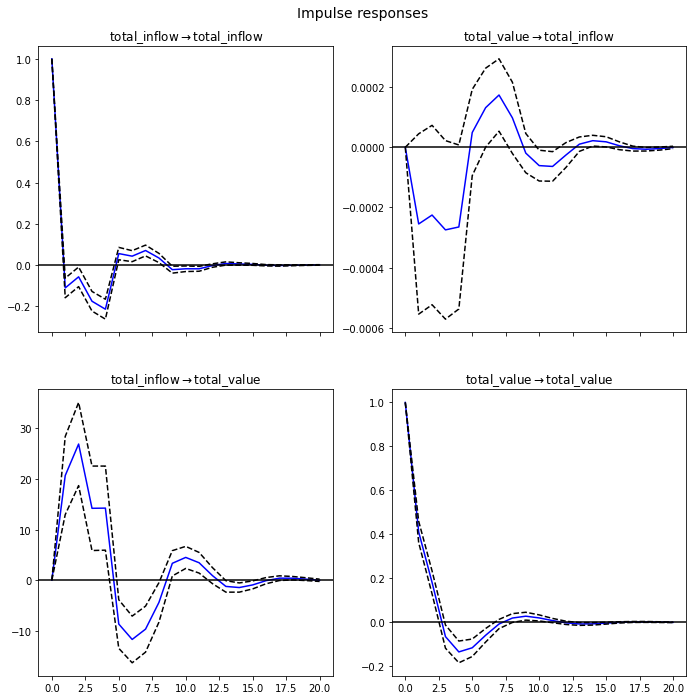
\includegraphics[width=1.15\textwidth]{irf_value.png}}
    \caption{北向资金净流入与沪深港通标的股成交额的双向脉冲响应函数（VAR(4) 模型，20阶）}
    \label{fig:irf_value}
    \vspace{0.5em}
    \begin{minipage}{0.95\textwidth}
        \small\textit{注：图中展示了基于 VAR(4) 模型估计的双向脉冲响应函数。左上子图为北向资金去趋势净流入（$\widetilde{\emph{Inflow}}_t$）受自身单位标准差冲击后的动态响应；右上子图为成交额（$\widetilde{\emph{Value}}_t$）对北向资金净流入冲击的动态响应；左下子图为北向资金净流入对成交额冲击的动态响应；右下子图为成交额受自身冲击后的动态响应。阴影区域为基于渐近标准误计算的95\%置信带。横轴为滞后阶数（交易日），纵轴为响应变量的变动幅度。去趋势方法为5日移动平均滤波。}
    \end{minipage}
\end{figure}

图\ref{fig:irf_value}的脉冲响应函数结果揭示了一个具有明确方向性的非对称动态关系：

\textbf{成交额对北向资金净流入的冲击响应（右上子图）}：当北向资金净流入受到一个正向单位标准差冲击时，沪深港通标的股成交额在冲击发生后的第1至第4个交易日（约1周内）呈现出\textit{统计显著为正}的脉冲响应——95\%置信带的下界在前4阶均位于零以上。这意味着北向资金的异常净流入能够在短期内显著带动A股市场的整体交易活跃度，其影响在约1周后逐渐衰减至不显著水平。这一结果为北向资金通过信息释放和情绪传染机制引发内地投资者跟风交易（即\textbf{短期羊群效应}）的假说提供了直接的实证支持。

\textbf{北向资金净流入对成交额的冲击响应（左下子图）}：当成交额受到一个正向单位标准差冲击时，北向资金净流入在各阶上的脉冲响应系数虽然方向不一，但其95\%置信带在所有阶数上均\textit{包含零值}，未能达到统计显著性。这表明尽管格兰杰检验在联合 $F$ 检验意义上拒绝了"成交额不构成净流入的格兰杰原因"的原假设（$p = 0.002$），但从脉冲响应函数的逐阶分析来看，成交额冲击对北向资金净流入的影响在任何单一滞后期上均不具备统计显著性。这意味着市场交易活跃度的变动对北向资金后续交易决策的引导作用在经济意义上是微弱的。

综合以上两个方向的脉冲响应分析，我们可以得出以下结论：北向资金净流入与A股市场交易活跃度之间的动态关系呈现出显著的\textbf{非对称性}——北向资金的异常净流入能够在短期内（约4个交易日，即1周左右）显著提振A股市场的整体成交额，而市场成交额的变动则对北向资金的后续交易行为不产生显著影响。这一非对称的脉冲响应模式符合"北向资金作为信息领先者引发内地投资者跟风交易"的羊群效应假说：北向资金的方向性交易释放了被市场参与者（尤其是散户投资者）广泛关注的信号，这一信号通过财经媒体的快速传播触发了约1周时间窗口内的跟风买入或卖出行为，从而显著放大了市场的短期交易活跃度。值得注意的是，该羊群效应的持续时间（约4个交易日）与第\ref{sec:prediction_horizon}小节中发现的北向资金预测能力集中于短期（日频至周频）的结论高度吻合，从影响路径的角度进一步印证了北向资金的市场效应主要作用于短期价格动态。

\subsubsection{股票收益波动率的合理度量}
\label{sec:vol_measure}

在进行北向资金对股价波动率影响的实证分析之前，我们首先需要解决一个关键的方法论前置问题：如何在日频层面对个股收益波动率进行合理且高时效性的度量。理论上，最自然的波动率定义是个股收益率的方差（variance），但在我们的研究场景中，直接使用传统的样本方差估计量面临严重的实际困难。

\vspace{0.5em}
\noindent\textbf{样本方差的滞后性问题}

传统的样本方差估计需要依赖一个回溯窗口（lookback window）来计算。设窗口长度为 $n$ 个交易日，则在时刻 $t$ 的样本方差为过去 $n$ 个交易日收益率偏离均值的平方和的均值。这种基于窗口的估计方法引入了一个不可避免的\textbf{滞后效应}：当真实波动率在某一时刻发生突变时，样本方差需要经过约 $n/2$ 个交易日的延迟才能充分反映这一变化。

为直观说明这一问题，考虑如下简化情形。假设某只股票的日度收益率服从均值为零的正态分布，其方差在时刻 $T$ 发生一次结构性跳变：

\begin{equation}
    r_t \sim N(0,\, \sigma_1^2), \quad t \leq T
    \label{eq:stage_1}
\end{equation}

\begin{equation}
    r_t \sim N(0,\, \sigma_2^2), \quad t > T, \quad \sigma_2^2 \neq \sigma_1^2
    \label{eq:stage_2}
\end{equation}

由于日度收益率的无条件期望在实证上极其接近于零（对于单个交易日而言，期望收益率的量级约为 $10^{-4}$，远小于波动率的量级约为 $10^{-2}$），我们可以合理地将均值固定为零。此时，在时刻 $t$ 处的样本方差估计量简化为：

\begin{equation}
    \widehat{\text{Var}}_t = \frac{1}{n}\sum_{k=0}^{n-1} r_{t-k}^2
    \label{eq:calculate}
\end{equation}

在式\ref{eq:calculate}的框架下，真实波动率在时刻 $T$ 瞬间从 $\sigma_1^2$ 跳变至 $\sigma_2^2$，但样本方差 $\widehat{\text{Var}}_t$ 在 $t \in [T, T+n]$ 的时间段内只能\textit{逐步}从 $\sigma_1^2$ 过渡至 $\sigma_2^2$——因为窗口内同时包含了来自旧分布（式\ref{eq:stage_1}）和新分布（式\ref{eq:stage_2}）的样本点。直到 $t = T + n$ 时，窗口内的所有样本才完全来自新分布，样本方差才能完整反映真实的波动率水平。平均而言，这一过渡过程引入了约 $n/2$ 个交易日的延迟。

\vspace{0.5em}
\noindent\textbf{滞后性对本研究的特殊挑战}

上述滞后效应在本研究的场景中尤为棘手。北向资金的日度净流入数据变化迅速且方向频繁切换——在大部分历史时段中，北向资金并不呈现出持续数周或数月的单向净流入或净流出态势，而是在日度层面上频繁交替。如果我们选择较长的样本方差窗口（例如 $n = 10$ 个交易日），则样本方差相对于真实波动率存在约5个交易日（即1周）的平均延迟。这意味着，当我们计算北向资金日度净流入与样本方差之间的相关性时，实际度量的是北向资金当日净流入与约1周前/后真实波动率之间的关系，而非当日的即时关系，这种时间错位将严重扭曲因果推断的有效性。

然而，若转而选择较短的窗口，则会同时引发两个新的统计问题。\textbf{问题一（高方差问题）}：样本方差本身是一个估计量，其抽样方差（即"方差的方差"）与窗口长度 $n$ 成反比。设单个平方收益 $r_t^2$ 的方差为 $\tau^2$，则在零均值假设下样本方差 $\widehat{\text{Var}}_t$ 的抽样方差近似为 $\tau^2 / n$。当 $n$ 较小时，$\widehat{\text{Var}}_t$ 的抽样噪声急剧增大，严重削弱后续相关性分析和因果检验的统计功效。\textbf{问题二（均值偏离问题）}：当窗口长度较短时，窗口内的样本均值 $\bar{r}_t = \frac{1}{n}\sum_{k=0}^{n-1}r_{t-k}$ 偏离理论均值零的概率显著增加。若使用标准的样本方差公式 $\widehat{\text{Var}}_t = \frac{1}{n-1}\sum_{k=0}^{n-1}(r_{t-k} - \bar{r}_t)^2$，在样本均值偶然偏离零时，该估计量将系统性地\textit{低估}真实波动率（因为部分波动被错误地归因于均值偏移而非离散程度）。

\vspace{0.5em}
\noindent\textbf{波动率代理指标的构建}

上述两个问题并非无解。基于以上分析，我们设计了第一个日频波动率代理指标 $\text{Vol}_1$，定义为个股当日收盘价与上一交易日收盘价计算出的日度回报率的平方\footnote{从样本方差的角度理解，$\text{Vol}_1$ 等价于将窗口长度缩减至极限值 $n = 1$，并在零均值假设下计算的"样本方差"。这种极端化处理彻底消除了滞后性问题，同时通过后文所述的横截面平均策略来补偿由此带来的高方差问题。}：

\begin{equation}
    \text{Vol}_{1,i,t} = r_{i,t}^2
    \label{eq:vol1}
\end{equation}

$\text{Vol}_1$ 指标的理论合理性建立在以下假设之上：对于股票 $i$，其日度回报率 $r_{i,t}$ 是一个均值为零的随机变量\footnote{严格而言，股票收益率的经验分布通常呈现尖峰厚尾特征，对数正态分布或 Student-$t$ 分布可能是比简单高斯分布更为准确的刻画。然而，此处的论证仅依赖于 $E[r_{i,t}] = 0$ 这一条件（日频下近似成立），而不依赖于特定的分布族假设。即使假设 $r_{i,t} \sim G(0, \sigma_{i,t}^2, \boldsymbol{\theta})$——其中 $G$ 为满足零均值和方差为 $\sigma_{i,t}^2$ 的一般分布族，$\boldsymbol{\theta}$ 为控制高阶矩特征的参数向量——以下推导仍然成立。}，即 $E[r_{i,t}] = 0$。在此假设下：

\begin{equation}
    E[\text{Vol}_{1,i,t}] = E[r_{i,t}^2] = E[r_{i,t}^2] - (E[r_{i,t}])^2 = \text{Var}(r_{i,t}) = \sigma_{i,t}^2
    \label{eq:vol1_unbiased}
\end{equation}

\noindent 式\ref{eq:vol1_unbiased}表明，$\text{Vol}_1$ 是真实波动率 $\sigma_{i,t}^2$ 的\textbf{无偏估计量}，从而解决了前述的问题二（均值偏离导致的系统性低估）。至于问题一（高方差），由于 $n = 1$ 时单个 $r_{i,t}^2$ 的抽样噪声确实很大，我们通过在数据层面进行补偿：不再仅使用市场指数级别的汇总数据（样本量为1），而是利用全部沪深港通标的\textbf{个股}层面的数据，在横截面上对 $\text{Vol}_{1,i,t}$ 进行平均或其他汇总操作。由于横截面上包含数千只标的股票，横截面平均能够将单个估计量的高方差有效地降低至可接受的水平（根据大数定律，横截面平均的方差以 $O(1/N)$ 的速率趋近于零，其中 $N$ 为标的股票数量）。

$\text{Vol}_1$ 指标虽然在理论上具有良好的统计性质，但作为我们根据研究需求自行构建的非标准指标，其实证稳健性尚需通过与既有文献中广泛使用的传统指标进行交叉验证来确认。为此，我们引入第二个波动率代理指标 $\text{Vol}_2$——\textbf{日内价格振幅}（intraday price range），定义为：

\begin{equation}
    \text{Vol}_{2,i,t} = \frac{P_{i,t}^{\text{high}} - P_{i,t}^{\text{low}}}{P_{i,t}^{\text{open}}}
    \label{eq:vol2}
\end{equation}

\noindent 其中 $P_{i,t}^{\text{high}}$、$P_{i,t}^{\text{low}}$、$P_{i,t}^{\text{open}}$ 分别为股票 $i$ 在交易日 $t$ 的最高价、最低价和开盘价。日内价格振幅是技术分析和市场微观结构文献中广泛使用的波动率代理指标，其优势在于直观性强且不依赖于分布假设。然而，相较于 $\text{Vol}_1$，$\text{Vol}_2$ 存在一个明显的局限性：作为一个纯粹的\textbf{日内指标}，$\text{Vol}_2$ 仅能捕捉交易时段内（即当日开盘至收盘）的价格波动，而完全忽略了前一交易日收盘至当日开盘之间的\textbf{隔夜价格波动}（overnight volatility）。在A股市场中，由于T+1交易制度、涨跌停板限制以及重大信息通常在收盘后发布等特征，隔夜价格跳变是股价波动的重要组成部分，不应被忽视。

鉴于 $\text{Vol}_1$ 和 $\text{Vol}_2$ 各有优劣且互为补充——$\text{Vol}_1$ 涵盖隔夜波动但理论基础非标准，$\text{Vol}_2$ 为传统指标但遗漏隔夜波动——我们将在接下来的因果检验分析中\textbf{同时使用}这两种指标并行验证，以最大程度增强结论的稳健性。当两种指标的检验结果一致时，结论的可信度将大幅提升；当结果出现分歧时，我们将结合指标各自的统计性质进行审慎的综合判断。

\subsubsection{北向资金净流入对股票收益波动率的影响}
\label{sec:vol_impact}

在明确定义了波动率的日频度量指标后，本小节沿用第\ref{sec:return_impact}小节的 VAR—格兰杰因果检验—脉冲响应函数分析框架，考察北向资金净流入与A股股票波动率之间的动态因果关系。

\vspace{0.5em}
\noindent\textbf{净流入变量的调整}

在将 VAR 框架应用于波动率分析时，需要对北向资金净流入的汇总方式进行一项关键调整。在第\ref{sec:return_impact}小节的成交额分析中，我们直接将个股层面的北向资金净流入（正值代表净买入，负值代表净卖出）在横截面上求和，得到总体净流入。然而，在波动率分析的语境中，这种直接加总是不恰当的。其原因在于：就对股价波动率的潜在影响而言，北向资金的净买入和净卖出应当产生\textbf{同方向}的效应——无论是大规模的净买入冲击还是大规模的净卖出冲击，都有可能通过流动性冲击和信息释放机制加剧标的股票的价格波动。若采用代数加总（即正负相消），则个股层面的大规模净买入和大规模净卖出将相互抵消，导致总量层面的净流入指标严重低估北向资金实际的交易活跃强度。为此，我们对个股层面的北向资金净流入先取\textbf{绝对值}，再在横截面上求和，得到修正后的总量交易强度指标：

\begin{equation}
    \text{AbsInflow}_t = \sum_{i=1}^{N_t} \left|\Delta w_{i,t}\right|
    \label{eq:abs_inflow}
\end{equation}

\noindent 其中 $\Delta w_{i,t}$ 为股票 $i$ 在交易日 $t$ 的北向资金净流入金额，$N_t$ 为当日沪深港通标的股票总数。$\text{AbsInflow}_t$ 度量的是北向资金在交易日 $t$ 的\textit{总体交易活跃程度}，而非\textit{总体方向性敞口}。

随后，我们分别以 $\text{AbsInflow}_t$ 与横截面平均波动率（$\overline{\text{Vol}}_{1,t} = \frac{1}{N_t}\sum_{i}\text{Vol}_{1,i,t}$ 和 $\overline{\text{Vol}}_{2,t} = \frac{1}{N_t}\sum_{i}\text{Vol}_{2,i,t}$）为内生变量，按照与第\ref{sec:return_impact}小节相同的流程——去趋势处理、BIC 准则选择最优滞后阶数、估计 VAR 模型——分别进行双向格兰杰因果检验和脉冲响应函数分析。

\vspace{0.5em}
\noindent\textbf{基于 $\emph{Vol}_1$（日度回报率平方）的检验结果}

使用 $\text{Vol}_1$ 指标时，BIC 准则选择的最优滞后阶数为8阶，即 VAR(8) 模型。双向格兰杰因果检验结果如表\ref{tab:granger_vol_1_1}和表\ref{tab:granger_vol_1_2}所示。

\begin{table}[htbp]
    \centering
    \caption{格兰杰因果检验（$\text{Vol}_1$）：北向资金交易强度对横截面平均波动率的预测效应}
    \label{tab:granger_vol_1_1}
    \makebox[\textwidth][c]{%
    \begin{minipage}{1.05\textwidth}
        \centering
        \vspace{0.5em}
        \begin{minipage}{0.95\textwidth}
            \small 原假设 $H_0$：北向资金去趋势交易强度（$\widetilde{\text{AbsInflow}}_t$）不构成横截面平均 $\text{Vol}_1$（$\widetilde{\overline{\text{Vol}}}_{1,t}$）的格兰杰原因。\\[0.3em]
            检验结论：在5\%显著性水平下\textbf{未能拒绝}原假设。
        \end{minipage}
        \vspace{0.5em}
        \begin{tabular}{lccc}
            \toprule
            \textbf{$F$ 统计量} & \textbf{5\%临界值} & \textbf{$p$ 值} & \textbf{自由度（df）} \\
            \midrule
            1.628 & 1.941 & 0.112 & (8, 3182) \\
            \bottomrule
        \end{tabular}
        \vspace{0.5em}
        \begin{minipage}{0.95\textwidth}
            \footnotesize\textit{注：VAR(8) 模型。$F$ 统计量检验 $\widetilde{\text{AbsInflow}}$ 的8阶滞后项在 $\widetilde{\overline{\text{Vol}}}_1$ 方程中的联合显著性。}
        \end{minipage}
    \end{minipage}%
    }
\end{table}

\begin{table}[htbp]
    \centering
    \caption{格兰杰因果检验（$\text{Vol}_1$）：横截面平均波动率对北向资金交易强度的预测效应}
    \label{tab:granger_vol_1_2}
    \makebox[\textwidth][c]{%
    \begin{minipage}{1.05\textwidth}
        \centering
        \vspace{0.5em}
        \begin{minipage}{0.95\textwidth}
            \small 原假设 $H_0$：横截面平均 $\text{Vol}_1$（$\widetilde{\overline{\text{Vol}}}_{1,t}$）不构成北向资金去趋势交易强度（$\widetilde{\text{AbsInflow}}_t$）的格兰杰原因。\\[0.3em]
            检验结论：在5\%显著性水平下\textbf{拒绝}原假设。
        \end{minipage}
        \vspace{0.5em}
        \begin{tabular}{lccc}
            \toprule
            \textbf{$F$ 统计量} & \textbf{5\%临界值} & \textbf{$p$ 值} & \textbf{自由度（df）} \\
            \midrule
            2.557 & 1.941 & 0.009 & (8, 3182) \\
            \bottomrule
        \end{tabular}
        \vspace{0.5em}
        \begin{minipage}{0.95\textwidth}
            \footnotesize\textit{注：VAR(8) 模型。$F$ 统计量检验 $\widetilde{\overline{\text{Vol}}}_1$ 的8阶滞后项在 $\widetilde{\text{AbsInflow}}$ 方程中的联合显著性。}
        \end{minipage}
    \end{minipage}%
    }
\end{table}

\begin{figure}[htbp]
    \centering
    \makebox[\textwidth][c]{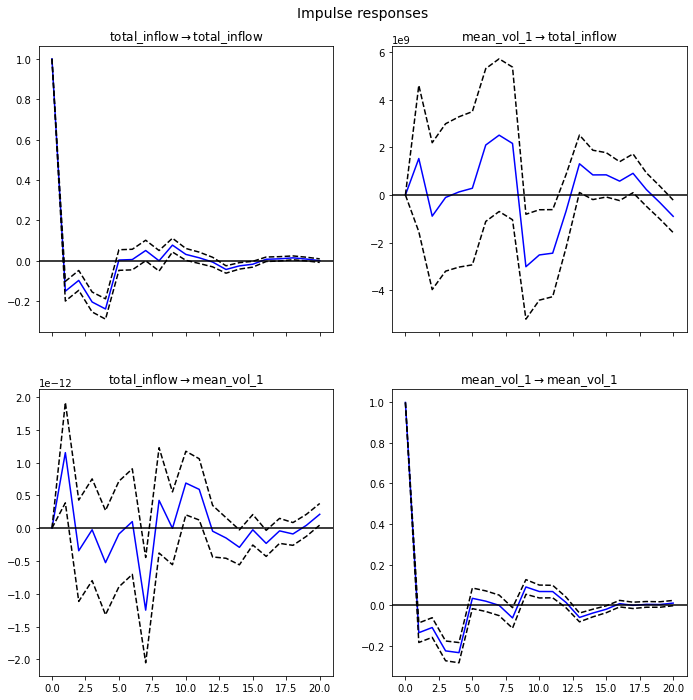
\includegraphics[width=1.15\textwidth]{irf_vol_1.png}}
    \caption{北向资金交易强度与横截面平均波动率（$\text{Vol}_1$）的双向脉冲响应函数（VAR(8) 模型，20阶）}
    \label{fig:irf_vol_1}
    \vspace{0.5em}
    \begin{minipage}{0.95\textwidth}
        \small\textit{注：波动率采用 $\emph{Vol}_1$（日度回报率平方）度量。图中展示了基于 VAR(8) 模型估计的双向脉冲响应函数，取前20阶。阴影区域为基于渐近标准误计算的95\%置信带。由于模型仅含两个内生变量，正交化处理对结果无实质性影响。北向资金交易强度为个股净流入绝对值的横截面求和（$\emph{AbsInflow}_t$）。}
    \end{minipage}
\end{figure}

\vspace{0.5em}
\noindent\textbf{基于 $\emph{Vol}_2$（日内价格振幅）的检验结果}

使用 $\text{Vol}_2$ 指标时，BIC 准则选择的最优滞后阶数为4阶，即 VAR(4) 模型。双向格兰杰因果检验结果如表\ref{tab:granger_vol_2_1}和表\ref{tab:granger_vol_2_2}所示。

\begin{table}[htbp]
    \centering
    \caption{格兰杰因果检验（$\text{Vol}_2$）：北向资金交易强度对横截面平均振幅的预测效应}
    \label{tab:granger_vol_2_1}
    \makebox[\textwidth][c]{%
    \begin{minipage}{1.05\textwidth}
        \centering
        \vspace{0.5em}
        \begin{minipage}{0.95\textwidth}
            \small 原假设 $H_0$：北向资金去趋势交易强度（$\widetilde{\text{AbsInflow}}_t$）不构成横截面平均 $\text{Vol}_2$（$\widetilde{\overline{\text{Vol}}}_{2,t}$）的格兰杰原因。\\[0.3em]
            检验结论：在5\%显著性水平下\textbf{拒绝}原假设。
        \end{minipage}
        \vspace{0.5em}
        \begin{tabular}{lccc}
            \toprule
            \textbf{$F$ 统计量} & \textbf{5\%临界值} & \textbf{$p$ 值} & \textbf{自由度（df）} \\
            \midrule
            14.86 & 2.375 & 0.000 & (4, 3206) \\
            \bottomrule
        \end{tabular}
        \vspace{0.5em}
        \begin{minipage}{0.95\textwidth}
            \footnotesize\textit{注：VAR(4) 模型。$F$ 统计量检验 $\widetilde{\text{AbsInflow}}$ 的4阶滞后项在 $\widetilde{\overline{\text{Vol}}}_2$ 方程中的联合显著性。}
        \end{minipage}
    \end{minipage}%
    }
\end{table}

\begin{table}[htbp]
    \centering
    \caption{格兰杰因果检验（$\text{Vol}_2$）：横截面平均振幅对北向资金交易强度的预测效应}
    \label{tab:granger_vol_2_2}
    \makebox[\textwidth][c]{%
    \begin{minipage}{1.05\textwidth}
        \centering
        \vspace{0.5em}
        \begin{minipage}{0.95\textwidth}
            \small 原假设 $H_0$：横截面平均 $\text{Vol}_2$（$\widetilde{\overline{\text{Vol}}}_{2,t}$）不构成北向资金去趋势交易强度（$\widetilde{\text{AbsInflow}}_t$）的格兰杰原因。\\[0.3em]
            检验结论：在5\%显著性水平下\textbf{未能拒绝}原假设。
        \end{minipage}
        \vspace{0.5em}
        \begin{tabular}{lccc}
            \toprule
            \textbf{$F$ 统计量} & \textbf{5\%临界值} & \textbf{$p$ 值} & \textbf{自由度（df）} \\
            \midrule
            0.252 & 2.375 & 0.909 & (4, 3206) \\
            \bottomrule
        \end{tabular}
        \vspace{0.5em}
        \begin{minipage}{0.95\textwidth}
            \footnotesize\textit{注：VAR(4) 模型。$F$ 统计量检验 $\widetilde{\overline{\text{Vol}}}_2$ 的4阶滞后项在 $\widetilde{\text{AbsInflow}}$ 方程中的联合显著性。}
        \end{minipage}
    \end{minipage}%
    }
\end{table}

\begin{figure}[htbp]
    \centering
    \makebox[\textwidth][c]{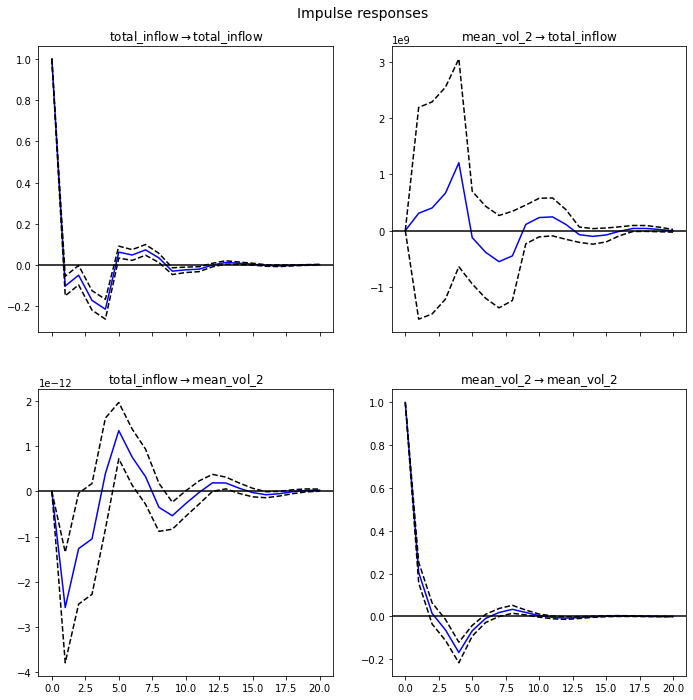
\includegraphics[width=1.15\textwidth]{irf_vol_2.png}}
    \caption{北向资金交易强度与横截面平均波动率（$\text{Vol}_2$）的双向脉冲响应函数（VAR(4) 模型，20阶）}
    \label{fig:irf_vol_2}
    \vspace{0.5em}
    \begin{minipage}{0.95\textwidth}
        \small\textit{注：波动率采用 $\emph{Vol}_2$（日内价格振幅）度量。图中展示了基于 VAR(4) 模型估计的双向脉冲响应函数，取前20阶。阴影区域为基于渐近标准误计算的95\%置信带。由于模型仅含两个内生变量，正交化处理对结果无实质性影响。北向资金交易强度为个股净流入绝对值的横截面求和（$\emph{AbsInflow}_t$）。}
    \end{minipage}
\end{figure}

\vspace{0.5em}
\noindent\textbf{结果综合分析}

将两种波动率指标的格兰杰因果检验结果进行交叉对比，可以发现以下不一致性：

\begin{enumerate}
    \item \textbf{北向资金交易强度 $\to$ 波动率方向}：使用 $\text{Vol}_1$ 时，原假设"交易强度不构成波动率的格兰杰原因"未能被拒绝（$F = 1.628$，$p = 0.112$）；但使用 $\text{Vol}_2$ 时，同方向的原假设被强烈拒绝（$F = 14.86$，$p < 0.001$）。两种指标给出了矛盾的结论。

    \item \textbf{波动率 $\to$ 北向资金交易强度方向}：使用 $\text{Vol}_1$ 时，原假设"波动率不构成交易强度的格兰杰原因"被拒绝（$F = 2.557$，$p = 0.009$）；但使用 $\text{Vol}_2$ 时，同方向的原假设未能被拒绝（$F = 0.252$，$p = 0.909$）。两种指标再次给出了矛盾的结论。
\end{enumerate}

两种指标在格兰杰因果检验的两个方向上均未能达成一致性结论，这本身已对任何单一方向上的因果关系主张构成了严重质疑。

进一步审视脉冲响应函数的估计结果（图\ref{fig:irf_vol_1}和图\ref{fig:irf_vol_2}），无论使用 $\text{Vol}_1$ 还是 $\text{Vol}_2$，在两个因果方向上，各阶脉冲响应系数的95\%置信带均未能\textit{一致且持续地}排除零值。具体而言，虽然个别阶数上的点估计值可能偏离零，但置信带始终包含零，且响应系数的符号在相邻阶数之间频繁切换，未呈现出如第\ref{sec:return_impact}小节中成交额响应函数那样清晰且持续的正向响应模式。这意味着即使在格兰杰检验中检测到了统计显著性（如 $\text{Vol}_2$ 下的交易强度→波动率方向），这种"格兰杰因果关系"也并未转化为经济意义上清晰、持续的动态影响路径。

\vspace{0.5em}
\noindent\textbf{小结}

综上所述，基于 VAR 模型框架下的格兰杰因果检验和脉冲响应函数分析，我们\textbf{未能提供}充分且一致的实证证据来支持北向资金的净交易活动对A股股票波动率产生直接的、统计显著且经济意义上可辨识的因果影响，反之亦然。两种波动率指标在格兰杰检验结果上的不一致性，以及脉冲响应函数在各阶上的不显著性，共同表明：在总量层面的线性 VAR 框架下，北向资金交易强度与A股市场波动率之间不存在稳健的动态因果关系。

这一"零结果"（null result）本身具有重要的信息价值，但需要审慎解读。一方面，它可能暗示北向资金对A股市场的影响并非通过直接的"交易量→波动率"线性传导机制实现，而可能通过更为间接和复杂的渠道发挥作用——例如通过改变投资者情绪结构、影响信息不对称程度、或在特定市场状态（如极端行情）下产生非线性的条件效应。另一方面，这一结果也提示我们，当前的总量层面线性 VAR 分析框架可能不足以捕捉北向资金与波动率之间潜在的复杂关系——例如，影响可能集中于特定股票群体（如北向资金重仓股）、特定市场状态（如高波动率区间）或特定交易日类型（如MSCI指数调整日），而这些条件性效应在总量层面的分析中被平均化和稀释了。这些可能性为后续研究中采用面板回归、分位数回归、状态依赖模型等更精细的实证工具提供了动机和方向。  

\subsubsection{北向资金交易行为对股票收益波动率的系统性影响}
\label{sec:vol_systematic}

上一小节（第\ref{sec:vol_impact}小节）基于 VAR—格兰杰因果检验—脉冲响应函数框架得出的初步结论是：北向资金在某一个交易日内交易规模的边际变动（多买或少买）并不会对A股股票收益波动率产生统计显著且稳健的即期因果影响。然而，这一"流量效应"的缺失并不排除另一种更为根本性的影响渠道——即北向资金\textbf{是否被允许交易}某只股票（即该股票是否被纳入沪深港通标的范围）这一\textbf{制度安排本身}，是否会系统性地改变该股票的波动率水平？这是一个与上一小节在分析层次上截然不同的问题：上一小节考察的是北向资金日度交易\textit{流量}的边际效应（intensive margin），而本小节考察的是北向资金交易\textit{准入资格}的整体效应（extensive margin）。

\vspace{0.5em}
\noindent\textbf{研究设计：基于沪港通开通的双重差分法}

为识别上述制度层面的因果效应，我们利用2014年11月17日\textbf{沪港通正式开通}这一准自然实验（quasi-natural experiment），采用双重差分法（Difference-in-Differences, DID）进行因果推断。沪港通开通是中国资本市场对外开放的标志性事件，首次允许境外投资者通过香港联合交易所直接买卖上海证券交易所的特定A股标的。这一政策事件的优势在于：第一，政策实施时点明确且外生于个股层面的波动率变化；第二，仅有部分沪市A股被纳入首批沪港通标的，而其余沪市A股未被纳入，从而自然地形成了实验组与对照组的分组结构。

由于我们所能获取的沪港通个股层面持仓数据最早从2017年10月开始，无法覆盖2014年的沪港通开通事件。因此，我们选择 DID 方法——该方法不依赖于个股层面的北向资金持仓或交易数据，仅需利用"是否被纳入沪港通标的"这一分组变量和政策实施时点来识别因果效应。

\vspace{0.5em}
\noindent\textbf{样本构建与数据处理}

样本的构建遵循以下步骤。首先，我们以事件窗口期（2014年5月17日至2015年5月17日，即政策实施前后各6个月）为基准，筛选出在窗口期首日和末日均处于正常上市状态的全部沪市A股，取其交集作为初始样本\footnote{尽管部分股票可能在事件窗口期内经历了短暂停牌后复牌的情形，但鉴于此类情况涉及的股票数量有限且停牌时段通常较短，我们在此简化处理中假设交集内的股票在整个事件窗口期内均处于正常交易状态。这一简化不会对 DID 估计的有效性产生实质性影响。}。

其次，我们将2014年11月18日至2015年5月17日期间\textit{新增纳入}或\textit{被调出}沪港通标的股范围的标的予以剔除。这一剔除基于以下考虑：沪港通开通仅两周后（2014年12月1日），沪港通标的股即经历了首次样本调整。由于调整时点距离政策开通极近，这些在短期内经历标的身份变化的股票可能具有某些特殊属性（例如被调入可能是因为满足了流动性或市值的阶段性门槛），将其纳入 DID 分析可能引入选择偏误（selection bias）。考虑到我们的总样本量仍然充裕，直接剔除这些边界案例是最为稳妥的处理方式。

经过上述筛选，最终样本包含\textbf{747只}沪市A股\footnote{这一数量并非由于大量剔除所致。事实上，截至2014年末，沪市A股上市公司总数尚不足1,000家。}，其中\textbf{467只}为首批沪港通标的股（\textbf{实验组}，即 $D_i = 1$），其余\textbf{280只}未被纳入沪港通（\textbf{对照组}，即 $D_i = 0$）。此外，我们将2014年11月17日（沪港通开通当日）的数据予以剔除，因为无法确定沪港通交易通道的精确启用时点（开盘前还是收盘后），该日的政策状态（$\text{post}$）存在不确定性\footnote{沪港通于2014年11月17日正式启动，但关于当日交易时段的具体安排，不同信息来源的表述存在细微差异。为避免将该日错误归类，我们采取保守策略直接剔除。}。最后，我们进一步收集了样本股票在事件窗口期内的日度行情数据（收盘价、最高价、最低价、开盘价）、年度财务数据（总资产、资产负债率、流动比率、资产收益率、资产周转率）以及申万一级行业分类信息，用于后续回归中的控制变量。

\vspace{0.5em}
\noindent\textbf{定性观察：实验组与对照组波动率差异的时序演变}

在进行严格的计量分析之前，我们首先进行定性的可视化观察，以直观把握沪港通开通前后实验组与对照组波动率差异的变化趋势，为后续的 DID 回归提供初步的方向性预判。

具体方法如下：以第\ref{sec:vol_measure}小节定义的 $\text{Vol}_1$（日度回报率平方）和 $\text{Vol}_2$（日内价格振幅）作为波动率度量，分别计算每个交易日实验组（沪港通标的股）的横截面平均波动率与对照组（非标的股）的横截面平均波动率之差。若该差值在沪港通开通日前后出现了系统性的水平跃升\footnote{严格而言，判断差值是否发生"系统性变化"需要进行正式的统计检验（如 Chow 结构性断点检验或 $t$ 检验），但此处仅作定性的视觉分析，正式检验将在后续的 DID 回归中完成。}，则初步表明北向资金的制度性准入可能导致了标的股票波动率的系统性变化。两种波动率指标下的差值时序图分别如图\ref{fig:vol_did_1}和图\ref{fig:vol_did_2}所示。

\begin{figure}[htbp]
    \centering
    \makebox[\textwidth][c]{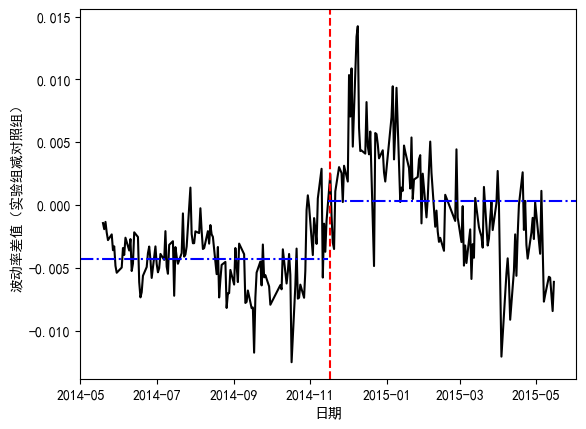
\includegraphics[width=1.15\textwidth]{vol_1.png}}
    \caption{沪港通开通前后实验组与对照组横截面平均波动率之差的时序演变（$\text{Vol}_1$：日度回报率平方）}
    \label{fig:vol_did_1}
    \vspace{0.5em}
    \begin{minipage}{0.95\textwidth}
        \small\textit{注：纵轴为每个交易日实验组（首批沪港通标的股，467只）的横截面平均 $\emph{Vol}_1$ 减去对照组（非标的股，280只）的横截面平均 $\emph{Vol}_1$。红色竖虚线标示沪港通正式开通日（2014年11月17日）；蓝色水平点划线分别表示开通前和开通后两个子区间内差值序列的均值。差值均值在开通后出现了向上的水平跃升。}
    \end{minipage}
\end{figure}

\begin{figure}[htbp]
    \centering
    \makebox[\textwidth][c]{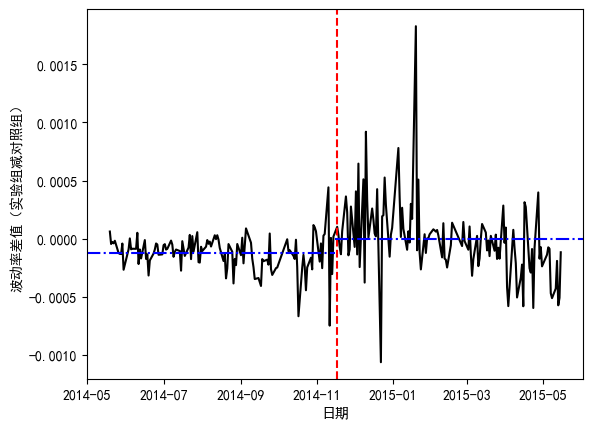
\includegraphics[width=1.15\textwidth]{vol_2.png}}
    \caption{沪港通开通前后实验组与对照组横截面平均波动率之差的时序演变（$\text{Vol}_2$：日内价格振幅）}
    \label{fig:vol_did_2}
    \vspace{0.5em}
    \begin{minipage}{0.95\textwidth}
        \small\textit{注：纵轴为每个交易日实验组横截面平均 $\emph{Vol}_2$ 减去对照组横截面平均 $\emph{Vol}_2$。其余标注含义同图\ref{fig:vol_did_1}。两种波动率指标均显示开通后实验组相对于对照组的波动率出现了系统性上升。}
    \end{minipage}
\end{figure}

图\ref{fig:vol_did_1}和图\ref{fig:vol_did_2}所展示的定性模式具有高度一致性：无论使用 $\text{Vol}_1$ 还是 $\text{Vol}_2$ 度量波动率，实验组相对于对照组的横截面平均波动率之差在沪港通开通后均出现了可辨识的向上跃升——开通后的均值线（蓝色点划线）明显高于开通前的均值线。这一跨指标一致的视觉模式初步暗示：北向资金交易准入的制度性变化可能导致了被纳入沪港通标的范围的股票相对波动率的系统性上升。

\vspace{0.5em}
\noindent\textbf{DID 回归模型设定}

在定性观察的基础上，我们构建正式的双重差分回归模型进行定量检验。设 $D_i$ 为分组虚拟变量（股票 $i$ 被纳入首批沪港通标的时取1，否则取0），$\text{post}_t$ 为时间虚拟变量（交易日 $t$ 在2014年11月17日之后取1，之前取0）。基准 DID 回归方程为：

\begin{equation}
    \text{Vol}_{i,t} = \beta_0 + \beta_1 D_i + \beta_2 \,\text{post}_t + \beta_3 \,D_i \times \text{post}_t + \varepsilon_{i,t}
    \label{eq:did_basic}
\end{equation}

\noindent 其中，$\text{Vol}_{i,t}$ 为股票 $i$ 在交易日 $t$ 的波动率（分别以 $\text{Vol}_1$ 和 $\text{Vol}_2$ 度量），$\beta_0$ 为截距项，$\beta_1$ 捕捉实验组与对照组在政策实施前即已存在的波动率水平差异（组间固有差异），$\beta_2$ 捕捉政策实施前后所有股票共同经历的波动率变化（时间趋势），$\beta_3$ 为\textbf{核心关注系数}——即 DID 估计量，度量的是在控制组间固有差异和共同时间趋势后，沪港通标的股在政策开通后相对于非标的股所经历的\textit{额外}波动率变化，$\varepsilon_{i,t}$ 为误差项。

然而，式\ref{eq:did_basic}的基准设定存在两个可能威胁内部有效性的识别问题：

\begin{enumerate}
    \item \textbf{组间系统性差异（选择偏误）}：实验组与对照组并非随机分组。公开资料显示，首批沪港通标的股的选择标准是将上证180指数、上证380指数成分股以及同时在沪港两地上市的A+H股纳入开放范围。这一选择标准导致实验组系统性地偏向于大市值、高流动性、机构持仓比例较高的蓝筹股，而对照组则以中小市值、低流动性的非指数成分股为主。这种组间的系统性差异可能通过公司基本面特征间接影响波动率水平，从而对 DID 估计产生混淆（confounding）。

    \item \textbf{时间维度的系统性扰动}：在我们的事件窗口期内（2014年5月至2015年5月），A股市场经历了2014年下半年开始的快速上涨行情（即"2014--2015年大牛市"的前半段）。尽管2015年6月下旬爆发的杠杆股灾不在我们的窗口期之内，但牛市行情的酝酿和加速过程可能已在窗口期内对市场整体波动率水平产生了系统性的上行影响。若不对这种时间维度的共同冲击进行控制，$\beta_3$ 的估计可能吸收与沪港通政策无关的时间趋势效应。
\end{enumerate}

为应对上述两个识别威胁，我们在 DID 回归中引入\textbf{个体固定效应} $\alpha_i$ 和\textbf{时间固定效应} $\gamma_t$。个体固定效应通过控制每只股票不随时间变化的所有可观测和不可观测特征（如公司规模、行业属性、治理结构等），有效消除了组间系统性差异的混淆效应。时间固定效应通过控制每个交易日所有股票共同经历的市场层面冲击（如宏观经济波动、市场情绪变化、监管政策调整等），有效吸收了时间维度的系统性扰动。修正后的 DID 回归方程为：

\begin{equation}
    \text{Vol}_{i,t} = \alpha_i + \gamma_t + \beta_1 D_i + \beta_2 \,\text{post}_t + \beta_3 \,D_i \times \text{post}_t + \mathbf{X}_{i,t}^{\top}\boldsymbol{\delta} + \varepsilon_{i,t}
    \label{eq:did_fe}
\end{equation}

\noindent 其中 $\alpha_i$ 为个体固定效应，$\gamma_t$ 为时间固定效应，$\mathbf{X}_{i,t}$ 为控制变量向量（在不同模型设定中逐步加入总资产、资产负债率、流动比率、资产收益率、资产周转率以及申万一级行业虚拟变量），$\boldsymbol{\delta}$ 为控制变量的系数向量。需要注意的是，在同时包含个体固定效应和时间固定效应的设定下，$D_i$（不随时间变化的组间差异）被个体固定效应吸收，$\text{post}_t$（不随个体变化的时间趋势）被时间固定效应吸收，因此 $\beta_1$ 和 $\beta_2$ 在实际估计中不可单独识别\footnote{在含固定效应的面板回归中，$D_i$ 和 $\text{post}_t$ 分别被 $\alpha_i$ 和 $\gamma_t$ 完美共线吸收。我们在表中仍保留这两个系数的报告以保持 DID 框架的完整性，但其估计值的解释需结合固定效应的存在审慎理解。}，核心识别仍来自交互项 $D_i \times \text{post}_t$ 的系数 $\beta_3$。

\vspace{0.5em}
\noindent\textbf{回归结果}

我们分别以 $\text{Vol}_1$ 和 $\text{Vol}_2$ 为因变量，在三种逐步加入控制变量的模型设定下估计式\ref{eq:did_fe}，共得到6组回归结果，汇总于表\ref{tab:did_main}中。

\begin{table}[htbp]
    \footnotesize
    \centering
    \caption{沪港通开通对标的股票波动率的影响：双重差分回归结果（完整样本窗口）}
    \label{tab:did_main}
    \makebox[\textwidth][c]{%
    \begin{minipage}{1.2\textwidth}
        \centering
        \begin{tabular}{lcccccc}
            \toprule
            & (1) & (2) & (3) & (4) & (5) & (6) \\
            \midrule
            & \multicolumn{3}{c}{\textbf{Panel A：因变量 $\text{Vol}_1$}} & \multicolumn{3}{c}{\textbf{Panel B：因变量 $\text{Vol}_2$}} \\
            \cmidrule(lr){2-4} \cmidrule(lr){5-7}
            & 基准模型 & 加入财务 & 加入全部 & 基准模型 & 加入财务 & 加入全部 \\
            \midrule
            常数项 & 0.0330*** & 0.0342*** & 0.0332*** & 0.0006*** & 0.0007*** & 0.0007*** \\
            & (0.000) & (0.001) & (0.002) & (8.74e-06) & (0.000) & (0.000) \\[0.3em]
            Post & 0.0211*** & 0.0210*** & 0.0211*** & 0.0008*** & 0.0008*** & 0.0008*** \\
            & (0.001) & (0.001) & (0.001) & (5.87e-05) & (5.88e-05) & (5.89e-05) \\[0.3em]
            Experiment & 0.0046*** & $-$0.0038*** & $-$0.0039*** & 9.83e-05 & $-$9.565e-05** & $-$9.192e-05** \\
            & (0.001) & (0.001) & (0.001) & (0.000) & (4.24e-05) & (4.25e-05) \\[0.3em]
            \textbf{Post $\times$ Experiment} & \textbf{0.0040***} & \textbf{0.0039***} & \textbf{0.0039***} & \textbf{9.82e-05***} & \textbf{9.751e-05***} & \textbf{9.763e-05***} \\
            & (0.000) & (0.000) & (0.000) & (1.6e-05) & (1.6e-05) & (1.6e-05) \\[0.3em]
            Total Assets & & 2.208e-14 & 2.395e-14 & & $-$1.142e-16 & 1.705e-15 \\
            & & (1.55e-14) & (1.55e-14) & & (1.27e-15) & (1.27e-15) \\[0.3em]
            Leverage & & $-$0.0003 & $-$0.0007 & & 0.0002 & 0.0002 \\
            & & (0.002) & (0.002) & & (0.000) & (0.000) \\[0.3em]
            Current Ratio & & $-$0.0044** & $-$0.0047** & & $-$0.0005** & $-$0.0004** \\
            & & (0.002) & (0.002) & & (0.000) & (0.000) \\[0.3em]
            ROA & & & $-$0.0009 & & & 1.595e-05 \\
            & & & (0.001) & & & (4.73e-05) \\[0.3em]
            Sales on Assets & & & 0.0023*** & & & $-$7.376e-05 \\
            & & & (0.001) & & & (6.46e-05) \\[0.3em]
            \midrule
            行业虚拟变量 & 否 & 是 & 是 & 否 & 是 & 是 \\
            个体固定效应 & 是 & 是 & 是 & 是 & 是 & 是 \\
            时间固定效应 & 是 & 是 & 是 & 是 & 是 & 是 \\
            \midrule
            观测值 & 165,058 & 165,058 & 165,058 & 165,058 & 165,058 & 165,058 \\
            $R^2$ & 0.320 & 0.320 & 0.320 & 0.136 & 0.136 & 0.136 \\
            \bottomrule
        \end{tabular}
        \vspace{0.5em}
        \begin{minipage}{0.95\textwidth}
            \footnotesize\textit{注：***、**、*分别表示在1\%、5\%、10\%的显著性水平上统计显著。括号内为聚类稳健标准误。样本区间为2014年5月17日至2015年5月17日（剔除2014年11月17日当日数据），共覆盖747只沪市A股。Panel A 和 Panel B 分别以 $\emph{Vol}_1$（日度回报率平方）和 $\emph{Vol}_2$（日内价格振幅）作为因变量。"行业虚拟变量"为基于申万一级行业分类的哑变量组。财务数据取自上市公司年报：2014年年报发布前使用2013年年报数据，发布后更新为2014年年报数据。\textbf{核心关注系数为 Post $\times$ Experiment（加粗行）}。}
        \end{minipage}
    \end{minipage}%
    }
\end{table}

表\ref{tab:did_main}的回归结果呈现出高度一致且稳健的模式。\textbf{核心关注系数} $\hat{\beta}_3$（Post $\times$ Experiment）在所有6组模型设定中均为\textbf{正值}且在\textbf{1\%的显著性水平下高度显著}。具体而言，在 Panel A（$\text{Vol}_1$）中，$\hat{\beta}_3$ 的估计值在三种模型设定下分别为 0.0040、0.0039 和 0.0039，表明沪港通标的股在政策开通后，其日度回报率平方（$\text{Vol}_1$）相对于非标的股平均增加了约 0.004 个单位。在 Panel B（$\text{Vol}_2$）中，$\hat{\beta}_3$ 的估计值分别为 $9.82 \times 10^{-5}$、$9.751 \times 10^{-5}$ 和 $9.763 \times 10^{-5}$，同样显著为正。

更为重要的是，$\hat{\beta}_3$ 的点估计值和显著性水平在从模型1/4（仅含固定效应的基准模型）到模型3/6（逐步加入总资产、资产负债率、流动比率、ROA、资产周转率及行业虚拟变量的完整模型）的过程中保持了极高的\textbf{稳定性}——系数值几乎不随控制变量的加入而变化，显著性水平始终维持在1\%以下。这种对控制变量设定的高度不敏感性表明，DID 估计量 $\hat{\beta}_3$ 捕捉到的是一个稳健的因果效应，而非由遗漏变量偏误（omitted variable bias）驱动的虚假关系。

\vspace{0.5em}
\noindent\textbf{稳健性检验：剔除事件临近期的窗口缩减分析}

尽管上述 DID 结果在统计意义上高度稳健，但一种合理的替代解释（alternative explanation）需要被正式排除——即\textbf{波动率暂时性回落假说}。这一假说的核心论点是：沪港通开通后标的股票波动率的上升可能仅仅是\textit{暂时性}的过渡现象，其成因是北向资金对新开放标的的初始交易热情——在从"零交易"到"允许交易"的制度转变（即从0到1的转变）发生后的最初一段时间内，大量境外投资者集中涌入建仓，产生了异常的流动性冲击和交易量放大效应，暂时性地推高了标的股票的波动率。但随着初始建仓期结束、市场对新制度安排完成适应性调整后，波动率将逐渐回落至正常水平。若这一假说成立，则 $\hat{\beta}_3$ 所反映的并非北向资金交易准入对波动率的\textit{持续性}系统效应，而仅仅是制度转换初期的\textit{暂时性}过渡效应，其政策含义将大相径庭。

值得指出的是，上述暂时性回落假说在表面上与图\ref{fig:vol_did_1}和图\ref{fig:vol_did_2}的定性观察亦可兼容——若开通后的差值均值主要由初始期的高波动率拉升，则即使长期差值已回落，均值线仍可能高于开通前。

为检验该替代假说，我们的首要回应如下：表\ref{tab:did_main}的回归样本覆盖了政策实施前后各6个月的完整窗口期（共约1年）。若 $\hat{\beta}_3$ 的显著性完全由开通后初始几周的暂时性波动率飙升所驱动，那么当窗口期延长至6个月时，初始期的高波动率观测值在整个"政策后"子样本中的权重已被显著稀释。换言之，在长达6个月的政策后窗口中，$\hat{\beta}_3$ 仍然高度显著，这本身已是波动率上升不完全归因于暂时性因素的间接证据。

为进一步提供更为直接的证据，我们进行如下稳健性检验：从原始样本中\textbf{剔除事件发生前后各1个月}（即2014年10月17日至2014年12月17日）的所有观测值，仅保留距离事件时点至少1个月以上的数据，然后在缩减后的样本上重新估计式\ref{eq:did_fe}。这一处理的逻辑是：若波动率上升确实仅为暂时性现象，则在剔除了初始过渡期数据后，$\hat{\beta}_3$ 应当变为不显著或大幅缩小。反之，若 $\hat{\beta}_3$ 在缩减样本中仍保持显著，则表明波动率上升具有\textit{持续性}特征，暂时性因素不足以完全解释观测到的效应。缩减窗口回归的结果如表\ref{tab:did_robust}所示。

\begin{table}[htbp]
    \footnotesize
    \centering
    \caption{沪港通开通对标的股票波动率的影响：双重差分回归结果（剔除事件前后各1个月的缩减样本窗口）}
    \label{tab:did_robust}
    \makebox[\textwidth][c]{%
    \begin{minipage}{1.2\textwidth}
        \centering
        \begin{tabular}{lcccccc}
            \toprule
            & (1) & (2) & (3) & (4) & (5) & (6) \\
            \midrule
            & \multicolumn{3}{c}{\textbf{Panel A：因变量 $\text{Vol}_1$}} & \multicolumn{3}{c}{\textbf{Panel B：因变量 $\text{Vol}_2$}} \\
            \cmidrule(lr){2-4} \cmidrule(lr){5-7}
            & 基准模型 & 加入财务 & 加入全部 & 基准模型 & 加入财务 & 加入全部 \\
            \midrule
            常数项 & 0.0317*** & 0.0331*** & 0.0321*** & 0.0006*** & 0.0006*** & 0.0006*** \\
            & (0.000) & (0.002) & (0.002) & (9.48e-06) & (0.000) & (0.000) \\[0.3em]
            Post & 0.0228*** & 0.0226*** & 0.0227*** & 0.0009*** & 0.0009*** & 0.0009*** \\
            & (0.001) & (0.001) & (0.001) & (5.85e-05) & (5.86e-05) & (5.86e-05) \\[0.3em]
            Experiment & 0.0054*** & $-$0.0049*** & $-$0.0050*** & 0.0001 & $-$0.0001*** & $-$0.0001*** \\
            & (0.001) & (0.001) & (0.001) & (0.000) & (4.32e-05) & (4.34e-05) \\[0.3em]
            \textbf{Post $\times$ Experiment} & \textbf{0.0034***} & \textbf{0.0033***} & \textbf{0.0033***} & \textbf{6.837e-05***} & \textbf{6.53e-05***} & \textbf{6.548e-05***} \\
            & (0.000) & (0.000) & (0.000) & (1.75e-05) & (1.75e-05) & (1.75e-05) \\[0.3em]
            Total Assets & & 5.962e-14*** & 6.177e-14*** & & 1.746e-15 & 1.713e-15 \\
            & & (1.57e-14) & (1.57e-14) & & (1.28e-15) & (1.28e-15) \\[0.3em]
            Leverage & & $-$0.0001 & $-$0.0006 & & 0.0003* & 0.0003* \\
            & & (0.002) & (0.002) & & (0.000) & (0.000) \\[0.3em]
            Current Ratio & & $-$0.0054** & $-$0.0058** & & $-$0.0005*** & $-$0.0005** \\
            & & (0.002) & (0.002) & & (0.000) & (0.000) \\[0.3em]
            ROA & & & $-$0.0009 & & & 1.169e-05 \\
            & & & (0.001) & & & (4.87e-05) \\[0.3em]
            Sales on Assets & & & 0.0024*** & & & $-$5.663e-05 \\
            & & & (0.001) & & & (6.5e-05) \\[0.3em]
            \midrule
            行业虚拟变量 & 否 & 是 & 是 & 否 & 是 & 是 \\
            个体固定效应 & 是 & 是 & 是 & 是 & 是 & 是 \\
            时间固定效应 & 是 & 是 & 是 & 是 & 是 & 是 \\
            \midrule
            观测值 & 136,604 & 136,604 & 136,604 & 136,604 & 136,604 & 136,604 \\
            $R^2$ & 0.320 & 0.320 & 0.320 & 0.141 & 0.141 & 0.141 \\
            \bottomrule
        \end{tabular}
        \vspace{0.5em}
        \begin{minipage}{0.95\textwidth}
            \footnotesize\textit{注：***、**、*分别表示在1\%、5\%、10\%的显著性水平上统计显著。括号内为聚类稳健标准误。样本区间为2014年5月17日至2014年10月17日以及2014年12月17日至2015年5月17日，即剔除了沪港通开通前后各1个月的数据（共约2个月的过渡期观测值被移除）。剔除后样本量从165,058降至136,604。其余设定同表\ref{tab:did_main}。\textbf{核心关注系数为 Post $\times$ Experiment（加粗行）}。}
        \end{minipage}
    \end{minipage}%
    }
\end{table}

表\ref{tab:did_robust}的稳健性检验结果清晰地表明：在剔除事件前后各1个月的过渡期数据后，核心 DID 系数 $\hat{\beta}_3$（Post $\times$ Experiment）在所有6组模型设定中仍然保持\textbf{正值}且在\textbf{1\%的显著性水平下高度显著}。在 Panel A（$\text{Vol}_1$）中，$\hat{\beta}_3$ 的点估计值从完整窗口（表\ref{tab:did_main}）的0.0039--0.0040略微下降至0.0033--0.0034，降幅约为15\%--17\%。在 Panel B（$\text{Vol}_2$）中，$\hat{\beta}_3$ 从 $9.75 \times 10^{-5}$--$9.82 \times 10^{-5}$ 下降至 $6.53 \times 10^{-5}$--$6.84 \times 10^{-5}$，降幅约为30\%--33\%。

上述比较结果可以做如下综合解读。$\hat{\beta}_3$ 在剔除过渡期后出现了一定程度的下降，这表明波动率暂时性回落假说并非完全没有道理——北向资金初始建仓期的集中交易确实在一定程度上贡献了 $\hat{\beta}_3$ 的估计值。然而，这一贡献远非全部：即使在完全移除了事件前后各1个月（共约2个月过渡期）的全部观测值后，$\hat{\beta}_3$ 仍保持高度显著，且点估计值仅下降了15\%--33\%，大部分效应在远离事件时点的数值中依然稳健存在。这一结果有力地表明，表\ref{tab:did_main}中 $\hat{\beta}_3$ 所捕捉到的效应\textbf{不能完全归因于}制度转换初期的暂时性波动率飙升，而是同时包含了北向资金交易准入对标的股票波动率产生的\textbf{持续性系统效应}。

\vspace{0.5em}
\noindent\textbf{小结}

综合完整窗口回归（表\ref{tab:did_main}）和缩减窗口稳健性检验（表\ref{tab:did_robust}）的结果，我们得出以下结论：基于沪港通2014年11月正式开通这一准自然实验的双重差分分析提供了强有力且稳健的实证证据，表明\textbf{北向资金交易准入的制度性变化导致了被纳入沪港通标的范围的A股股票收益波动率的系统性上升}。这一效应在控制个体固定效应、时间固定效应以及多种公司层面财务特征后依然显著，且在剔除事件过渡期数据后仍保持稳健，表明其并非仅由初始建仓期的暂时性交易冲击所驱动，而是反映了境外投资者交易行为对A股市场微观结构产生的持续性影响。

这一发现与前文对北向资金交易特征的系统性刻画形成了逻辑上的闭环：北向资金以高换手率、择时驱动为主导的交易模式（第\ref{subsec:return_decomposition}和\ref{sec:trading_pattern}小节），加之其信息优势高度集中于短期价格波动预测（第\ref{sec:prediction_horizon}小节），使其交易行为在客观上具备了放大标的股票短期波动性的潜力。沪港通开通后标的股票波动率的系统性上升，正是这种潜力在制度层面从"不可交易"转变为"可交易"后的现实体现。

\newpage
\section{策略设计与回测分析}
\label{sec:strategy}

在本部分中，我们将基于前文对北向资金交易特征的系统性实证发现，构建一个具有经济价值且可实际交易的量化选股策略。正如文献综述部分所述，既有研究已广泛记录了北向资金净流量与A股当日及短期回报率之间的正向相关关系，但以往文献中提出的基于北向资金信号的策略均存在一个共同的方法论缺陷：未能检验其超额收益是否独立于\textbf{动量—反转策略}（泛指一切利用滞后收益率构造的alpha信号）。这一遗漏在A股市场的制度背景下尤为关键，原因如下。

在A股市场中，动量—反转策略在\textit{纸面上}（即在原始回报率或去风格化回报率的IC检验中）往往呈现出极强的预测效力，但其对应的损益（PnL）在很大程度上是\textbf{不可实现的虚假PnL}。这一虚假性源于A股市场两项核心制度特征的共同作用：

\begin{enumerate}
    \item \textbf{卖空限制}（short-selling constraints）：A股市场上，投资者不能自由地对个股进行卖空操作\footnote{虽然融资融券制度允许对少数标的进行融券卖空，但融券标的范围极为有限、融券费率高昂且券源稀缺，在实务中远不能满足系统性做空的需求。}。这意味着价格被高估的股票若要使价格回归基本面价值，只能依赖存量持有人的主动出售，而无法通过卖空机制加速价格调整。由于存量出售是一个受制于投资者行为偏差（如"处置效应"，即被套牢的持有人倾向于继续持有亏损头寸以避免确认损失）的缓慢过程，A股的下跌动量（negative momentum）显著弱于上涨动量（positive momentum），导致动量策略的信息系数（IC）往往\textit{集中于空头端}——即策略的预测价值主要体现在识别未来表现最差的股票，而非识别表现最好的股票。然而，空头alpha在无法卖空的市场环境中是无法被主动交易捕获的。

    \item \textbf{涨跌停板制度}（price limit mechanism）：A股实行$\pm 10\%$（创业板和科创板为$\pm 20\%$）的每日涨跌幅限制。当重大新信息进入市场后，其对股价的冲击效应可能无法在当日完全反映于价格之中——若信息利好/利空的幅度超过涨跌停幅度，则剩余的价格调整将被延迟至后续交易日。这一机制人为地制造了虚假的短期动量信号：涨停/跌停后的数日内，股价大概率延续同方向趋势（即所谓的"打板效应"）。然而，在涨停/跌停当日的收盘时点，买卖双方通常存在大量的排队"封单"（即无法成交的挂单），导致投资者在该时点上实际上无法按收盘价建仓或平仓，这种alpha同样是不可交易的。
\end{enumerate}

因此，若要构建一个在A股市场中\textit{真正可交易}的alpha策略，我们必须在方法论上解决上述问题。我们的核心做法是：在模型训练的\textbf{预测目标}层面，预先消除动量—反转策略的效应，使得模型所学习到的alpha信号\textit{完全独立于}任何基于滞后收益率的线性预测因子。

在量化投资工业界，策略模型的拟合目标通常并非原始回报率，而是一种经过风格因子调整后的\textbf{残差化回报率}（de-styled return），在Barra风险模型框架下通常被称为"de-Barra return"（以下简记为 bret）。Barra因子模型是由MSCI公司开发的一套多因子风险模型体系，其典型版本包含一个国家因子、约10个风格因子（涵盖市值、估值、动量、波动率、流动性、盈利质量等维度）以及约70个行业因子。所谓 de-Barra return，是指在每个横截面上将原始回报率对全部Barra因子进行线性回归后所得到的残差项——即剔除了Barra因子可解释部分后的回报率剩余成分。由于Barra的风格因子已包含动量因子（根据不同版本，动量因子的具体构造有所差异：主流版本仅包含52周累计回报率相关因子，而fast版本中还加入了短期回报因子）、市值因子、财务估值因子等，加之行业因子对行业共同效应的控制，只有收益来源\textit{有别于}上述已知风格、且在行业平均意义上产生超额回报的alpha信号，才能对 bret 具有预测能力。

我们在本研究中采用了与上述工业实践一脉相承的方法论：自行构造一组"类Barra"风格因子，将动量—反转等效应从预测目标中彻底剔除，确保模型所提取的alpha信号完全独立于滞后收益率的线性组合。

\vspace{0.5em}
\noindent\textbf{本部分结构}

本部分的组织结构如下：第\ref{sec:feature_engineering}小节介绍特征工程，包括预测目标与样本权重的定义方式以及特征变量的构造逻辑；第\ref{sec:linear_model}小节介绍线性模型的设定与滚动在线学习算法；第\ref{sec:evaluation}小节定义评价指标体系并展示线性模型的样本外回测结果；第\ref{sec:nonlinear}小节引入非线性梯度提升树模型，测试alpha的极限性能并讨论线性模型与非线性模型的比较结果。

\subsection{特征工程}
\label{sec:feature_engineering}

\subsubsection{预测目标与样本权重}
\label{sec:target_weight}

\paragraph{预测目标的构造}

对于预测目标的处理，我们首先使用每个交易日的收盘价计算个股的对数回报率 $r_{i,t} = \ln(P_{i,t}^{\text{close}}/P_{i,t-1}^{\text{close}})$。随后，我们自行构造了一组"类Barra"风格因子，用于对原始回报率进行截面残差化处理。选择自行构造而非直接使用商业Barra因子数据的原因有二：第一，商业Barra因子数据的获取成本高昂，对于本文的研究目的而言边际价值有限；第二，也是更为重要的原因，我们希望尽可能\textit{彻底地}剔除预测目标中的动量—反转效应，而自定义风格因子体系允许我们灵活地纳入更多与滞后收益率相关的因子维度，从而比标准Barra模型更为充分地消除动量—反转信号的残留。

具体而言，我们选取的用于残差化处理的风格因子列表如表\ref{tab:custom_barra_factors}所示。

\begin{table}[htbp]
    \centering
    \caption{用于预测目标残差化处理的自定义风格因子列表}
    \label{tab:custom_barra_factors}
    \makebox[\textwidth][c]{%
    \begin{tabular}{ll}
        \toprule
        \textbf{因子类别} & \textbf{因子名称与说明} \\
        \midrule
        价格动量因子 & 1日回报率、5日回报率、21日回报率、252日回报率 \\
        规模因子 & $\log(\text{流通市值})$（logMktCap） \\
        行业因子 & 2012版证监会行业分类代码（哑变量形式） \\
        \bottomrule
    \end{tabular}%
    }
    \vspace{0.5em}
    \begin{minipage}{0.95\textwidth}
        \footnotesize\textit{注：价格动量因子覆盖了从日频（1日）到年频（252日）的四个时间尺度，以尽可能完整地捕捉不同频率上的动量—反转效应。行业因子采用哑变量形式（而非Barra模型中常用的[0,1]连续暴露度），因此在截面回归中起到控制行业固定效应的作用。}
    \end{minipage}
\end{table}

此处需要说明一个技术细节：我们在截面回归中\textit{未包含常数项}（截距项）。在标准Barra模型中，国家因子通常可视为常数项，用于吸收截面均值。然而，由于我们的行业因子采用的是严格的哑变量形式（即每个行业对应一个取值为0或1的指示变量），全部行业哑变量之和恰好等于全1向量，若再加入常数项将导致\textbf{完全共线性}问题（perfect multicollinearity）。而在标准Barra模型中，行业因子并非哑变量，而是取值于$[0,1]$区间的连续变量（表示公司对各行业的"暴露度"），其各列之和不等于全1向量，因此不存在与常数项的共线性问题。在我们的设定下，行业哑变量组在功能上已\textit{等价地包含了}常数项的作用——这是因为行业哑变量的线性张成空间（column space）包含了全1向量。因此，残差化处理后得到的 bret 在每个横截面上的加权均值恒等于零\footnote{严格而言，这里的"加权均值为零"是在OLS回归意义下成立的，即 $\sum_{i} \hat{\varepsilon}_{i,t} = 0$（无权重时）或 $\sum_{i} w_i \hat{\varepsilon}_{i,t} = 0$（加权回归时），前提是回归设计矩阵的列空间包含全1向量。}，其经济含义是：bret 度量的是在市场基准、行业基准、动量—反转基准和市值风格基准上的\textbf{多重超额回报}。

分析表\ref{tab:custom_barra_factors}中的因子构成可以发现，我们纳入了1日、5日、21日和252日四个时间尺度的滞后收益率相关因子，分别对应日内反转、周度动量/反转、月度动量和年度动量等不同频率上的价格延续或反转效应。在截面残差化处理中剔除这些因子的线性影响后，剩余的 bret 在数学上\textit{正交于}上述四个滞后收益率因子的线性张成空间。这意味着：\textbf{任何仅仅是滞后价格的线性组合的特征，都不可能对 bret 产生线性预测能力}。这一性质从根本上保证了我们后续模型所提取的alpha信号独立于动量—反转效应，从而避免了前文分析的A股市场中动量alpha不可交易的问题。

\paragraph{样本权重的设定}

对于训练过程中的样本权重，我们采用了一种简洁的定义方式：每只股票在每个交易日的权重等于其\textbf{流通市值的对数}，即 $w_{i,t} = \log(\text{MktCap}_{i,t})$。这一权重分布的经验直方图如图\ref{fig:weight_distribution}所示。

\begin{figure}[htbp]
    \centering
    \makebox[\textwidth][c]{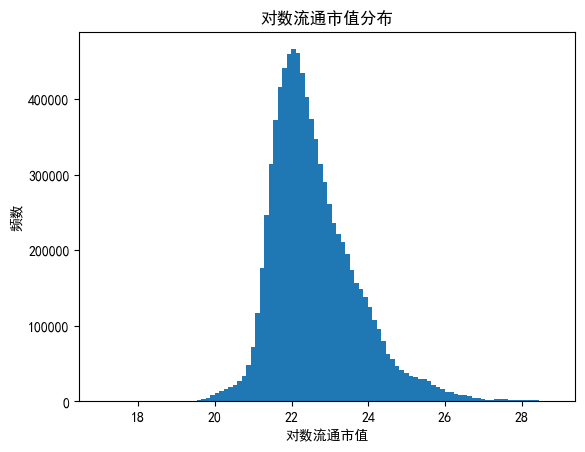
\includegraphics[width=1.15\textwidth]{../Figure/权重分布.png}}
    \caption{样本权重（对数流通市值）的横截面经验分布}
    \label{fig:weight_distribution}
    \vspace{0.5em}
    \begin{minipage}{0.95\textwidth}
        \small\textit{注：图中展示了某一典型交易日横截面上全部沪深港通标的股的 $\log(\emph{MktCap})$ 分布。该分布近似正态，最大值与最小值之间的差距相对温和（约为2--3倍），表明不同股票之间的权重差异被有效压缩。}
    \end{minipage}
\end{figure}

从图\ref{fig:weight_distribution}中可以观察到，对数市值权重在不同股票之间的差异相对温和，远小于直接使用原始市值权重（即线性市值加权）时的极端分化。这种权重设计的合理性体现在以下三个方面：

\begin{enumerate}
    \item \textbf{避免极端权重导致的有效样本量缩减}：若采用原始市值权重，少数超大市值股票（如工商银行、贵州茅台等）将占据绝对主导的权重份额，导致模型的训练过程被这些极少数个股所支配，有效利用的独立数据点大幅缩减。这一问题在非线性模型（如第\ref{sec:nonlinear}小节的梯度提升树）中尤为严重——当权重极度集中时，树模型的分裂节点将过度聚焦于高权重个股的特征分布，从而引发极为严重的过拟合问题。对数变换有效压缩了权重的分布范围，使模型能够更均匀地学习全市场个股的信息。

    \item \textbf{合理反映交易成本的差异化影响}：市值较大的股票通常具有更好的流动性（更窄的买卖价差、更深的订单簿深度），因此在实际交易中面临更低的冲击成本。赋予大市值股票略高的权重（但非线性放大），使得模型在训练时更重视那些在实务中alpha更容易被低成本捕获的标的，这与策略的可交易性目标相一致。

    \item \textbf{匹配北向资金的广覆盖交易特征}：第\ref{sec:trading_pattern}小节的实证分析已揭示，北向资金的交易模式具有高换手率、广泛分散化选股的特征，而非集中于少数蓝筹标的。若采用过于极端的市值加权方案，训练出的alpha将过度集中在少数大市值股票上，无法充分体现北向资金信息在广泛标的上的分散化预测价值。对数市值权重通过压缩权重差异，鼓励模型从更多标的中提取信号，与北向资金的实际行为模式更为匹配。
\end{enumerate}

\subsubsection{特征变量的构造}
\label{sec:feature_construction}

我们为模型训练准备的全部26个特征变量的定义汇总于表\ref{tab:feature_list}中。

\begin{table}[htbp]
    \centering
    \caption{模型训练特征变量一览：原始数据字段、运算操作与时间参数}
    \label{tab:feature_list}
    \makebox[\textwidth][c]{%
    \footnotesize
    \begin{tabular}{clllc}
        \toprule
        \textbf{编号} & \textbf{特征描述} & \textbf{原始数据字段} & \textbf{运算操作} & \textbf{半衰期} \\
        \midrule
        0  & 持仓市值的63日 ts-zscore 后 EMA & MarketValue & tsz(63) $\to$ EMA(63) & 0.1 \\
        1  & 净持仓变动的63日 ts-zscore 后 EMA & NetChangeValue & tsz(63) $\to$ EMA(63) & 0.1 \\
        2  & 持仓市值的 EMA / L2-norm 归一化 & MarketValue & EMA(63) / L2-norm(63) & 0.1 \\
        3  & 净持仓变动的 EMA / L2-norm 归一化 & NetChangeValue & EMA(63) / L2-norm(63) & 0.1 \\
        4  & 去价格因子残差化后的市值 tsz EMA & MarketValue & ret-residualize $\to$ tsz(63) $\to$ EMA(63) & 0.1 \\
        5  & 去价格因子残差化后的净变动 tsz EMA & NetChangeValue & ret-residualize $\to$ tsz(63) $\to$ EMA(63) & 0.1 \\
        \midrule
        6--11 & 同 feature 0--5 & 同上 & 同上 & 1 \\
        12--17 & 同 feature 0--5 & 同上 & 同上 & 5 \\
        18--23 & 同 feature 0--5 & 同上 & 同上 & 10 \\
        \midrule
        24 & RSI 变体：EMA(净变动) / EMA($|\text{净变动}|$) & NetChangeValue & EMA 比值 & 5 \\
        25 & RSI 变体：EMA(净变动) / EMA($|\text{净变动}|$) & NetChangeValue & EMA 比值 & 20 \\
        \bottomrule
    \end{tabular}%
    }
    \vspace{0.5em}
    \begin{minipage}{0.95\textwidth}
        \footnotesize\textit{注：tsz(63) 表示63个交易日窗口的时间序列 $z$-score 标准化（即减去窗口均值再除以窗口标准差）。EMA(63) 表示窗口长度为63个交易日的指数加权移动平均。L2-norm(63) 表示63个交易日窗口的 $L_2$ 范数。"ret-residualize"表示在截面上对1日、5日、21日回报率进行线性回归取残差。Feature 6--23 与 feature 0--5 具有相同的运算结构，仅 EMA 半衰期参数不同（分别为1、5、10个交易日）。所有特征在最终输入模型前均经过横截面 GaussianRank 变换，仅保留截面排序信息。}
    \end{minipage}
\end{table}

以下从设计动机和技术原理两个角度，对上述特征工程的核心逻辑进行阐述。

\vspace{0.5em}
\noindent\textbf{设计动机}

本文的特征设计严格遵循前文实证分析所揭示的北向资金行为特征进行定制化构造。第\ref{subsec:return_decomposition}--\ref{sec:prediction_horizon}小节的实证结果已明确表明：北向资金的超额收益主要来源于短期择时能力，而非长期价值投资式的持有收益；其信息优势高度集中于日频至周频的短期价格预测，且交易频率远超典型的机构投资者。基于这些发现，我们在特征构造中着重关注北向资金在每只标的股票上的\textbf{持仓净变化的时间序列动态特征}，而非持仓水平的静态截面分布。全部特征均基于两个核心原始数据字段派生：\textbf{持仓市值}（MarketValue，反映北向资金在各标的上的仓位规模）和\textbf{净持仓变动}（NetChangeValue，反映北向资金的日度调仓方向和力度）。

\vspace{0.5em}
\noindent\textbf{核心运算符及其技术原理}

\textit{1. 时间序列标准化（ts-zscore 与 L2-norm 归一化）}：为消除持仓市值和净持仓变动在时间序列上的长期趋势和水平效应（例如随A股市场整体市值的增长，北向资金的绝对持仓金额和净流入金额均呈上升趋势），我们采用63个交易日（约1个季度）窗口的时间序列 $z$-score（ts-zscore）进行标准化，将原始数据转换为相对于其近期历史分布的标准化偏离度。作为替代的归一化方案，我们同时使用了 L2-norm 归一化，即将 EMA 值除以同窗口的 $L_2$ 范数。

此处需要解释 L2-norm 归一化为何同样能够有效消除长期自相关（ACF）。关键在于特征构建流程的最后一步：所有特征在输入模型前均经过\textbf{横截面 GaussianRank 变换}，该变换仅保留每个横截面上特征值的\textit{排序}（ordinal）信息，而完全丢弃绝对数值信息。因此，对于任意标量函数 $g(\cdot)$，运算 $X / \text{L2-norm}(X)$ 与运算 $(X - g(\text{L2-norm}(X))) / g(\text{L2-norm}(X))$ 在经过 GaussianRank 后产生\textit{完全相同}的截面排序。特别地，取 $g$ 为恒等函数时，$X / \text{L2-norm}(X)$ 等价于 $(X - \text{L2-norm}(X)) / \text{L2-norm}(X)$，后者在形式上类似于以 L2-norm 为基准的"偏离度"。经过这种处理，特征在63个交易日尺度上的时间序列自相关（ACF）被有效压缩至接近零。

\textit{2. 多半衰期指数加权移动平均（EMA）}：在完成上述标准化处理后，我们对标准化后的"快速"特征（即已消除长期ACF的特征）施加不同半衰期的 EMA 平滑处理，半衰期分别设定为0.1、1、5和10个交易日。这一多尺度设计服务于两个目的：第一，不同半衰期的 EMA 能够捕捉北向资金行为在不同时间窗口（从日内级别到双周级别）中的差异化表现——例如，极短半衰期（0.1天）的 EMA 近似反映最近1--2天的信号，而较长半衰期（10天）的 EMA 则捕捉近两周的累积趋势。第二，当多个不同半衰期的 EMA 特征同时输入线性模型时，模型可以通过学习到类似 $\text{EMA}_{\text{long}} - \beta \cdot \text{EMA}_{\text{short}}$ 的权重组合，自动构造出类似于技术分析中 MACD（Moving Average Convergence Divergence）指标的差分信号，从而识别北向资金行为动态的加速或减速变化。

\textit{3. RSI 变体}：特征24和25为相对强弱指数（Relative Strength Index, RSI）的变体，定义为净持仓变动的 EMA 与净持仓变动绝对值的 EMA 之比。若忽略指数衰减的效应，这一指标在直觉上可理解为北向资金净持仓变动在给定窗口内的\textit{累计变化量}除以\textit{累计一阶变差}（total variation），其取值范围为 $[-1, 1]$。当指标值接近 $+1$ 时，表明北向资金在窗口期内\textit{稳定且持续地}净买入该标的（所有日度变动方向一致）；接近 $-1$ 时表示稳定持续的净卖出；接近0则表明窗口期内的净变动方向频繁交替，呈现震荡特征。这一指标的核心价值在于区分"大幅度但不稳定的净变动"与"小幅度但高度一致的净变动"——对于相同的期初期末持仓净变化，中间过程越曲折，RSI越接近0；过程越平稳，RSI的绝对值越大。

\textit{4. 滞后回报率残差化}：特征4--5、10--11、16--17和22--23在构造流程中加入了一个额外的截面残差化步骤——在每个交易日的横截面上，将持仓市值或净持仓变动对1日、5日、21日的滞后回报率进行线性回归，取残差作为特征值。这一操作的经济含义是构造"\textbf{控制滞后回报率后的北向资金持仓超额净变化}"。由于北向资金的持仓决策对标的近期价格表现具有显著的敏感性（即北向资金自身具有一定的动量追随行为），原始的持仓净变化中包含了反映滞后回报率的成分。而由于我们的预测目标 bret 已经剔除了滞后回报率的线性影响，原始特征中的这些成分只会增加模型参数的抽样波动性（方差），而无法提供额外的预测信息。因此，在特征层面预先剔除这些成分，能够提高信噪比并增强模型参数的稳定性。

\subsection{线性模型与滚动在线学习算法}
\label{sec:linear_model}

我们首先采用线性模型来检验上述特征工程的预测有效性。由于金融市场具有内在的\textbf{非平稳性}（non-stationarity）——即数据生成过程的统计特征（如条件均值、条件方差、变量间的相关结构等）随时间系统性地变化——使用固定参数的静态模型难以适应市场环境的动态演变。因此，我们采用\textbf{滚动 Ridge 回归}（rolling Ridge regression）的在线学习方式训练模型：在每一个交易日 $t$，模型参数 $\beta_t$ 均基于从数据起点到第 $t-1$ 天的全部历史数据进行估计，然后使用 $\beta_t$ 对第 $t$ 天的横截面特征进行预测。此外，为使模型参数更迅速地适应近期市场环境的变化，我们在训练过程中引入了\textbf{时间衰减权重}（temporal decay weight），赋予近期观测值更大的权重。

\subsubsection{模型设定}
\label{sec:linear_setup}

传统的机器学习建模框架通常将数据集显式划分为训练集、验证集和测试集三个互不重叠的子集：在训练集上估计模型参数，在验证集上调优超参数，最终在测试集上评估模型的泛化表现。然而，在金融时间序列的预测任务中，这种静态三分法面临两个根本性的局限：第一，单一静态模型的参数无法适应市场环境的持续变化，导致模型在训练集和测试集之间的性能差距（即"样本内—样本外落差"）通常较大且不可控；第二，验证集和测试集中的数据被完全隔离于训练过程之外，导致在数据量本就有限的金融场景中出现严重的数据利用效率损失。

我们采用的滚动回归范式有效克服了上述两个局限。其本质是一种\textbf{在线学习}（online learning）策略，选择这一范式的原因有二。第一，Ridge 回归的解析解形式天然适合在线增量更新——如下一小节将详细推导的那样，模型参数可以通过维护一个累积矩阵和累积向量的方式在每个交易日高效更新，而无需每次从头重新计算全部历史数据的回归，这使得在单线程环境下也能实现快速的日度参数更新。第二，滚动回归使得模型在每个交易日都充分利用了截至前一日的\textit{全部}历史数据，不存在传统框架中验证集和测试集数据被"浪费"的问题。更为重要的是，由于每一天的预测都是基于严格的历史信息集（不包含当天及未来的数据），滚动回归产生的预测结果不存在传统意义上的"样本内"部分——所有预测均为\textbf{真正的样本外预测}。

严格而言，Ridge 回归的正则化超参数 $\lambda$ 仍需调优，理论上应将数据划分为两部分：前一部分用于滚动回归的调参，后一部分作为真正未见的测试数据。然而，来自量化投资工业界的经验表明，$\lambda$ 参数对策略最终表现的影响在通常情况下并不大——这是因为在低信噪比的金融数据中，Ridge 正则化的主要功能是防止因特征共线性导致的参数爆炸，而非精细地平衡偏差与方差。因此，我们在本文中直接采用 $\lambda = 0.01$ 的经验值\footnote{这一取值在量化投资实务中被广泛使用，属于"温和正则化"的范围：足以抑制共线性导致的参数不稳定，但不会过度压缩参数向零从而损失过多的预测信号。}，未进行专门的超参数搜索过程。

\subsubsection{滚动在线学习算法}
\label{sec:rolling_algorithm}

Ridge 回归的优化目标函数为：
\begin{equation}
    \min_{\boldsymbol{\beta}} \sum_{i=1}^{n} w_i \left(y_i - \mathbf{x}_i^{\top} \boldsymbol{\beta}\right)^2 + \lambda \|\boldsymbol{\beta}\|_2^2
    \label{eq:ridge_obj}
\end{equation}

\noindent 其中 $y_i$ 为第 $i$ 个样本的预测目标（bret），$\mathbf{x}_i$ 为对应的特征向量，$w_i$ 为样本权重，$\lambda$ 为正则化参数，$\|\cdot\|_2$ 为 $L_2$ 范数。式\ref{eq:ridge_obj}的解析解为：

\begin{equation}
    \hat{\boldsymbol{\beta}} = \left(\mathbf{X}^{\top} \mathbf{W} \mathbf{X} + \lambda \mathbf{I}\right)^{-1} \mathbf{X}^{\top} \mathbf{W} \mathbf{y}
    \label{eq:ridge_solution}
\end{equation}

\noindent 其中 $\mathbf{X}$ 为设计矩阵（$n \times p$），$\mathbf{W} = \text{diag}(w_1, \ldots, w_n)$ 为样本权重的对角矩阵，$\mathbf{y}$ 为目标向量，$\mathbf{I}$ 为 $p \times p$ 单位矩阵。

在滚动回归的在线学习设定中，我们需要在每个交易日 $t$ 更新式\ref{eq:ridge_solution}中的解。核心思路是利用矩阵乘积的\textbf{可加性}（additivity），将累积计算拆分为逐日增量更新。具体而言，定义如下两个累积量：

\begin{equation}
    \mathbf{A}_t = \mathbf{X}_{1:t-1}^{\top} \mathbf{W}_{1:t-1} \mathbf{X}_{1:t-1} + \lambda \mathbf{I}, \qquad
    \mathbf{b}_t = \mathbf{X}_{1:t-1}^{\top} \mathbf{W}_{1:t-1} \mathbf{y}_{1:t-1}
    \label{eq:cumulative}
\end{equation}

\noindent 其中下标 $1:t-1$ 表示使用第1天至第 $t-1$ 天的全部数据。此时第 $t$ 天的模型参数为 $\hat{\boldsymbol{\beta}}_t = \mathbf{A}_t^{-1} \mathbf{b}_t$。

$\mathbf{A}_t$ 和 $\mathbf{b}_t$ 具有如下增量更新关系：

\begin{equation}
    \mathbf{A}_t = \mathbf{A}_{t-1} + \mathbf{X}_{t-1}^{\top} \mathbf{W}_{t-1} \mathbf{X}_{t-1}
    \label{eq:A_update}
\end{equation}

\begin{equation}
    \mathbf{b}_t = \mathbf{b}_{t-1} + \mathbf{X}_{t-1}^{\top} \mathbf{W}_{t-1} \mathbf{y}_{t-1}
    \label{eq:b_update}
\end{equation}

\noindent 其中 $\mathbf{X}_{t-1}$ 和 $\mathbf{y}_{t-1}$ 为第 $t-1$ 天的特征矩阵和目标向量，$\mathbf{W}_{t-1}$ 为该日的权重对角矩阵。因此，在实际代码实现中，每个交易日的操作流程为：（1）首先利用已有的 $\mathbf{A}_t$ 和 $\mathbf{b}_t$ 计算当日参数 $\hat{\boldsymbol{\beta}}_t = \mathbf{A}_t^{-1} \mathbf{b}_t$（此时累积量仅包含历史数据，不存在数据泄露）；（2）使用 $\hat{\boldsymbol{\beta}}_t$ 对当日横截面特征 $\mathbf{X}_t$ 进行预测，得到 alpha 预测值 $\hat{\mathbf{y}}_t = \mathbf{X}_t \hat{\boldsymbol{\beta}}_t$；（3）在当日交易结束后，利用 $\mathbf{X}_t$ 和 $\mathbf{y}_t$ 通过式\ref{eq:A_update}和\ref{eq:b_update}更新累积量，为次日的参数计算做准备。

\vspace{0.5em}
\noindent\textbf{时间衰减权重的实现}

为使模型更重视近期数据，我们在样本权重 $w_i$ 中引入时间衰减因子：对于在交易日 $s$ 产生的数据点，当模型在交易日 $t$（$t > s$）进行参数估计时，该数据点的有效权重为原始截面权重乘以指数衰减因子 $e^{-(t-s)/\tau}$，其中 $\tau$ 为衰减时间常数，与半衰期 $h$ 的关系为 $\tau = h / \ln 2$。我们设定半衰期 $h = 500$ 个交易日（约2年），即每经过500个交易日，历史数据点的有效权重衰减为原来的一半。

时间衰减权重与增量更新框架的兼容性依赖于权重矩阵 $\mathbf{W}$ 的\textbf{对角性质}。以两个交易日的数据为例：

\begin{equation}
\begin{split}
    \mathbf{X}_{1:2}^{\top} \mathbf{W}_{1:2} \mathbf{X}_{1:2} &=
    \begin{pmatrix} \mathbf{X}_1^{\top} & \mathbf{X}_2^{\top} \end{pmatrix}
    \begin{pmatrix} e^{-(t-1)/\tau} \mathbf{W}_1 & \mathbf{0} \\ \mathbf{0} & e^{-(t-2)/\tau} \mathbf{W}_2 \end{pmatrix}
    \begin{pmatrix} \mathbf{X}_1 \\ \mathbf{X}_2 \end{pmatrix} \\
    &= \mathbf{X}_1^{\top} \!\left(e^{-(t-1)/\tau} \mathbf{W}_1\right) \mathbf{X}_1 + \mathbf{X}_2^{\top} \!\left(e^{-(t-2)/\tau} \mathbf{W}_2\right) \mathbf{X}_2
\end{split}
    \label{eq:decay_example}
\end{equation}

\noindent 式\ref{eq:decay_example}表明，含时间衰减的累积矩阵仍然可以表示为逐日贡献的累加和。在实际实现中，我们只需在每个交易日的增量更新步骤之前，先将已有的累积量 $\mathbf{A}_{t-1}$ 和 $\mathbf{b}_{t-1}$ 整体乘以衰减因子 $e^{-1/\tau}$（将全部历史数据的权重统一衰减一步），然后再加上新一天的增量贡献，即可正确维护含时间衰减的累积量。

在上述在线学习过程中，模型在每个交易日 $t$ 动态输出预测结果 $\hat{\mathbf{y}}_t = \mathbf{X}_t \hat{\boldsymbol{\beta}}_t$，我们将这一逐日预测序列记为线性模型的\textbf{alpha 信号}。

\subsection{评价指标与回测结果}
\label{sec:evaluation}

在获得了模型的逐日alpha预测值后，我们需要建立一套定量的评价指标体系来评估alpha信号的质量。以下记 $\alpha_{i,t}$ 为第 $i$ 只股票在第 $t$ 个交易日的 alpha 预测值，$r_{i,t}$ 为该股票在第 $t$ 日的实际 bret 收益率，$w_{i,t}$ 为对应的样本权重。

\subsubsection{评价指标体系}

我们参照量化投资工业界的通行标准，定义如下三个核心评价指标：

\begin{itemize}
    \item \textbf{信息系数}（Information Coefficient, IC）：度量 alpha 预测值与实际收益率在横截面上的加权相关程度，定义为修正的加权相关系数：
    \begin{equation}
        \text{IC}_t = \frac{\sum_{i} w_{i,t}\, \alpha_{i,t}\, r_{i,t}}{\sqrt{\sum_{i} w_{i,t}\, \alpha_{i,t}^2}\;\sqrt{\sum_{i} w_{i,t}\, r_{i,t}^2}}
        \label{eq:ic}
    \end{equation}

    \item \textbf{标准化损益}（Standardized PnL, SP）：度量 alpha 信号在每单位预测强度下所产生的实际收益，定义为：
    \begin{equation}
        \text{SP}_t = \frac{\sum_{i} w_{i,t}\, \alpha_{i,t}\, r_{i,t}}{\sum_{i} w_{i,t}\, \alpha_{i,t}^2}
        \label{eq:sp}
    \end{equation}

    \item \textbf{自相关函数}（Autocorrelation Function, ACF）：度量 alpha 信号在时间序列上的持续性（高自相关性意味着策略的日度调仓幅度较小，从而交易成本更低），定义为：
    \begin{equation}
        \text{ACF}_k = \frac{\sum_{t}\left(\boldsymbol{\alpha}_t - \bar{\boldsymbol{\alpha}}\right)^{\top}\!\left(\boldsymbol{\alpha}_{t-k} - \bar{\boldsymbol{\alpha}}\right)}{\sum_{t}\left(\boldsymbol{\alpha}_t - \bar{\boldsymbol{\alpha}}\right)^{\top}\!\left(\boldsymbol{\alpha}_t - \bar{\boldsymbol{\alpha}}\right)}
        \label{eq:acf}
    \end{equation}
    其中 $\boldsymbol{\alpha}_t = (\alpha_{1,t}, \ldots, \alpha_{N_t,t})^{\top}$ 为交易日 $t$ 的 alpha 截面向量，$\bar{\boldsymbol{\alpha}}$ 为时间序列均值。
\end{itemize}

在后续的分析图表中，IC 图所绘制的是累积平均 IC 曲线 $\overline{\text{IC}}_t = \frac{1}{t}\sum_{\tau=1}^{t}\text{IC}_{\tau}$，SP 图绘制的是累积平均 SP 曲线 $\overline{\text{SP}}_t = \frac{1}{t}\sum_{\tau=1}^{t}\text{SP}_{\tau}$，以便直观展示alpha信号质量随时间的演变趋势。

\subsubsection{线性模型的样本外表现}
\label{sec:linear_results}

如前所述，在滚动在线学习框架下，线性模型不存在传统意义上的"样本内"回测——每一天的预测均为真正的样本外预测。我们直接展示全样本期间的回测结果如图\ref{fig:linear_ic}--\ref{fig:linear_acf}所示。

\begin{figure}[htbp]
    \centering
    \makebox[\textwidth][c]{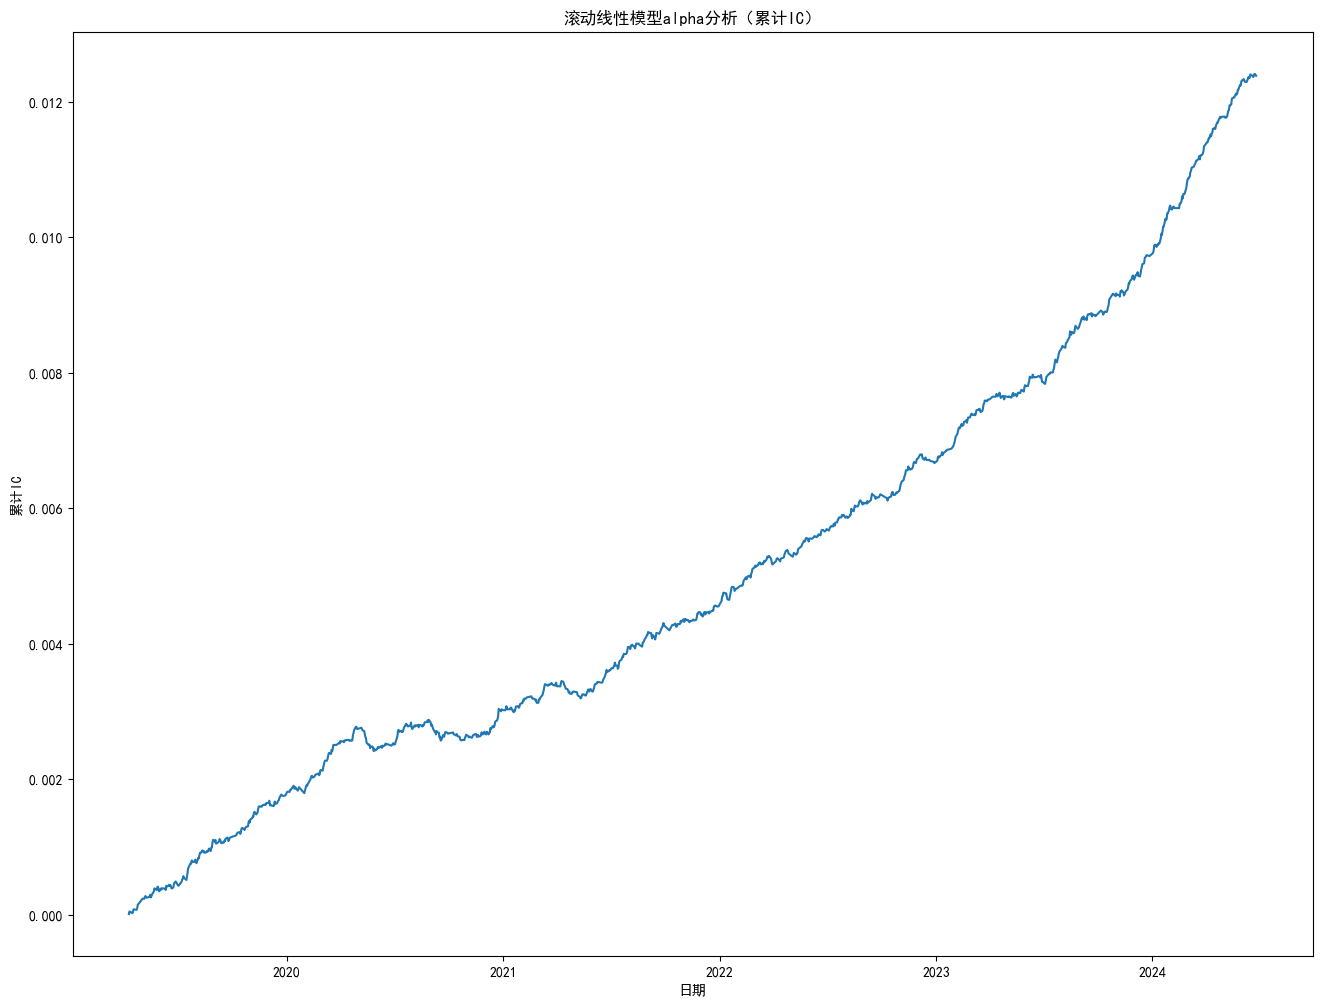
\includegraphics[width=1.15\textwidth]{../Figure/rollingWLS_IC.png}}
    \caption{滚动线性模型 alpha 的累积平均信息系数（IC）曲线}
    \label{fig:linear_ic}
    \vspace{0.5em}
    \begin{minipage}{0.95\textwidth}
        \small\textit{注：横轴为交易日期，纵轴为从回测起点到当日的累积平均 IC 值。IC 的计算基于式\ref{eq:ic}，预测目标为去动量、去市值、去行业的残差化回报率（bret）。累积平均 IC 从初期接近零逐步上升至约0.012并趋于稳定，表明模型持续产生正向且稳健的截面预测信号。}
    \end{minipage}
\end{figure}

\begin{figure}[htbp]
    \centering
    \makebox[\textwidth][c]{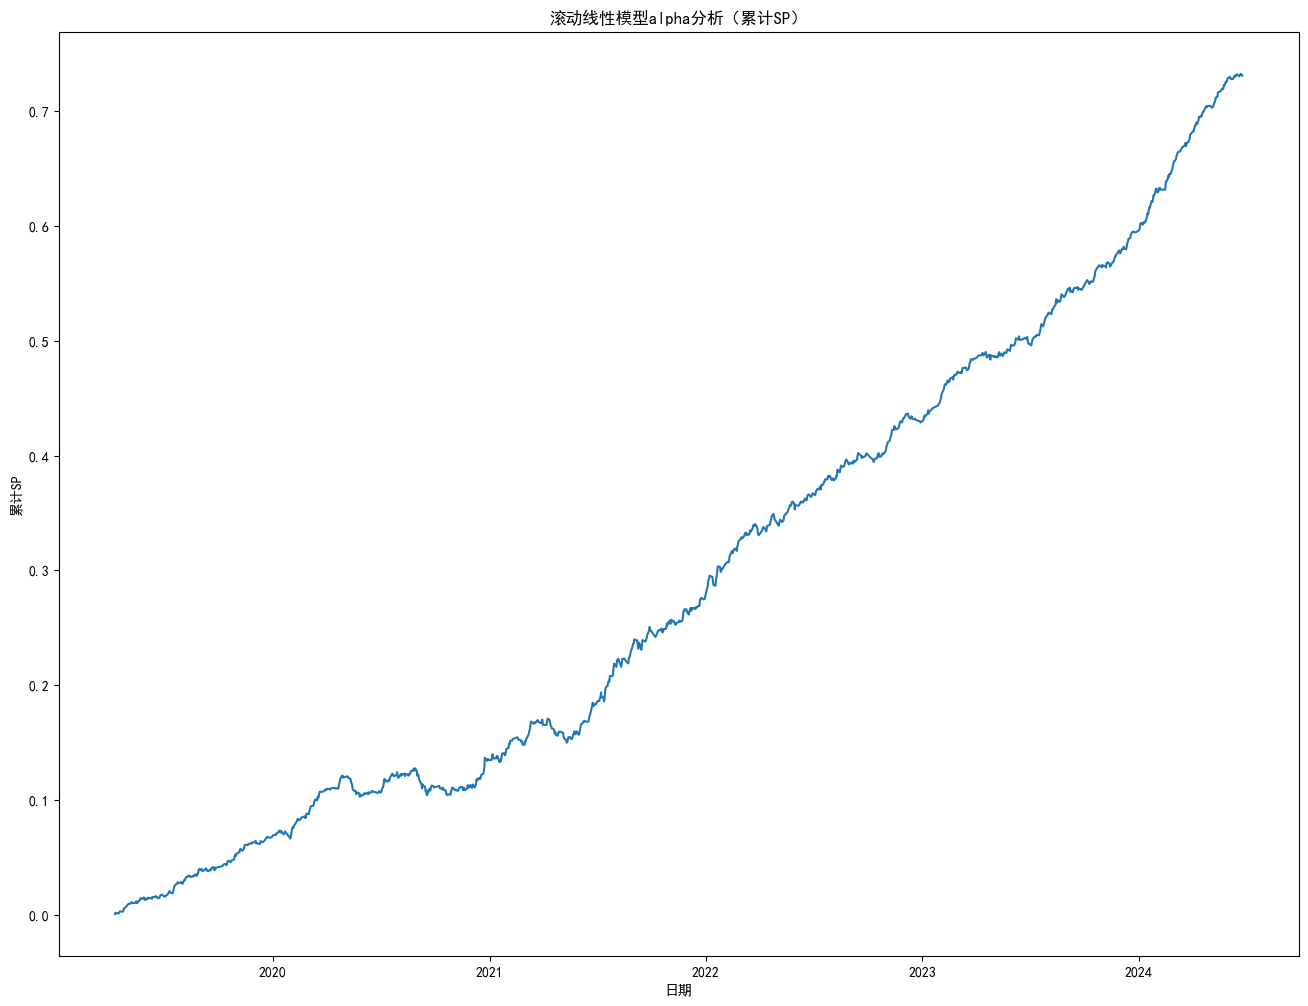
\includegraphics[width=1.15\textwidth]{../Figure/rollingWLS_SP.png}}
    \caption{滚动线性模型 alpha 的累积平均标准化损益（SP）曲线}
    \label{fig:linear_sp}
    \vspace{0.5em}
    \begin{minipage}{0.95\textwidth}
        \small\textit{注：横轴为交易日期，纵轴为从回测起点到当日的累积平均 SP 值（基于式\ref{eq:sp}）。累积平均 SP 呈现单调上升趋势，从2019年末的接近零攀升至2025年初的约0.73。策略实现了年化14.518\%的扣费前超额收益率与4.998的年化夏普比率。}
    \end{minipage}
\end{figure}

\begin{figure}[htbp]
    \centering
    \makebox[\textwidth][c]{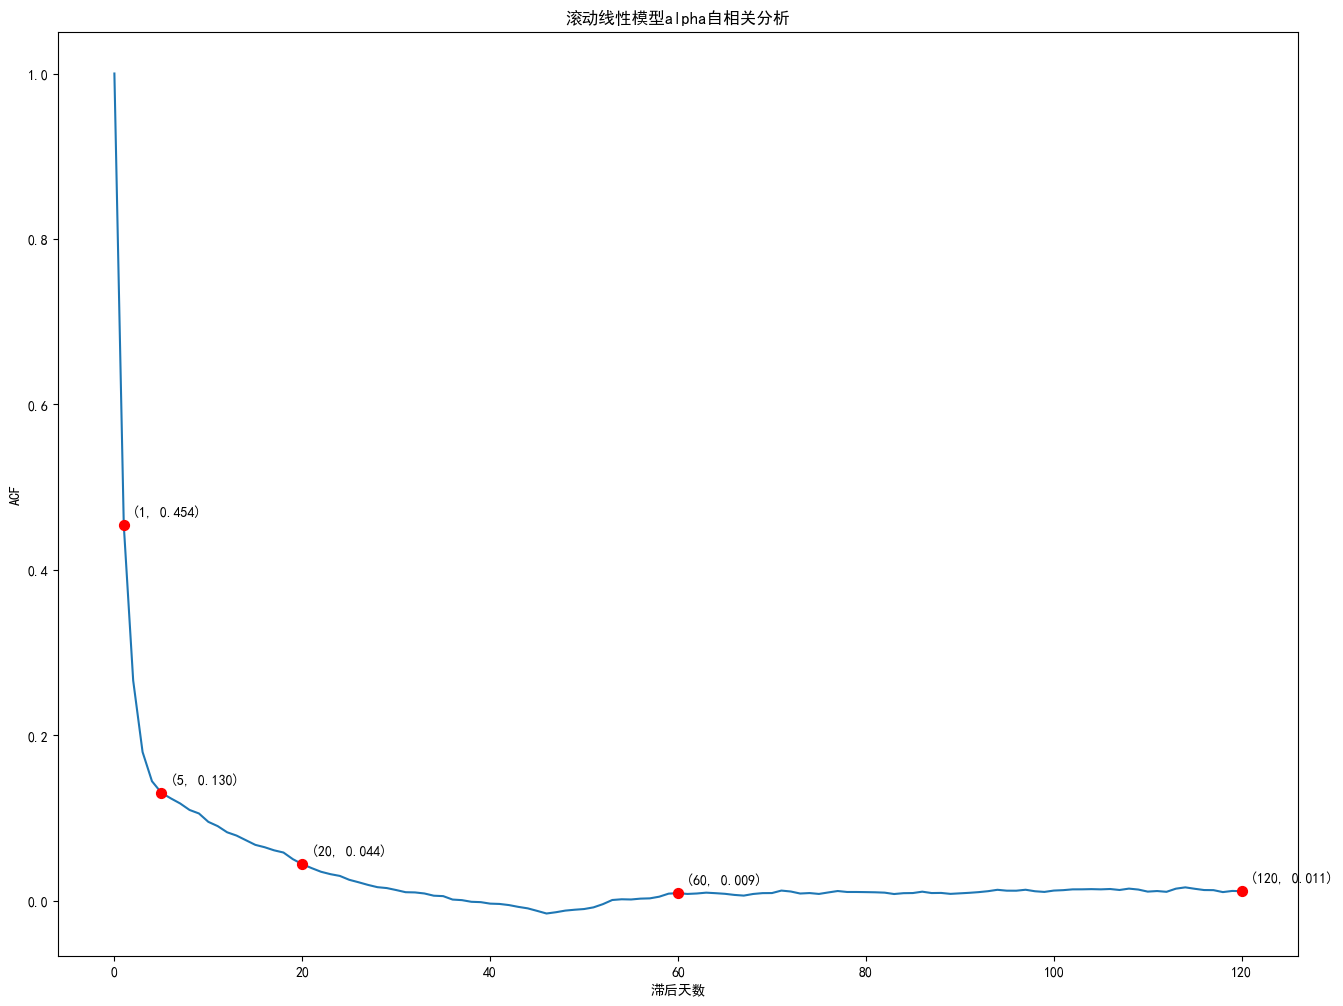
\includegraphics[width=1.15\textwidth]{../Figure/ACF.png}}
    \caption{滚动线性模型 alpha 信号的自相关函数（ACF）}
    \label{fig:linear_acf}
    \vspace{0.5em}
    \begin{minipage}{0.95\textwidth}
        \small\textit{注：横轴为滞后阶数（交易日），纵轴为 alpha 截面向量的自相关系数（基于式\ref{eq:acf}）。ACF 在滞后1日处为0.454，随后近似指数衰减：滞后5日降至0.130，滞后20日降至0.044，滞后120日接近0.011。}
    \end{minipage}
\end{figure}

从上述三个维度的定量指标来看，滚动线性模型展现出了令人满意的样本外表现。

\textbf{IC 分析}（图\ref{fig:linear_ic}）：累积平均 IC 从回测初期（2019--2020年）的接近零逐步上升至约0.012并趋于稳定。这一 IC 水平虽然从绝对数值上看较为温和，但需要在本研究的特定背景下加以理解。第一，我们已经在预测目标中\textit{预先剔除了}全部与滞后收益率线性相关的成分，这意味着传统技术分析中IC值较高的动量、反转等因子的贡献已被人为移除——剩余的可预测信号本身就十分微弱。第二，IC 值是在控制了市值风格、行业因子和市场因子后的\textit{多重超额}预测能力的度量，其基准线远高于使用原始回报率时的IC。第三，在量化投资实务中，日频IC哪怕仅为0.01量级，当策略具备足够高的换手率和精细的信号转化机制时，也能产生显著的商业价值——这正是后续SP指标所验证的。

\textbf{SP 分析}（图\ref{fig:linear_sp}）：累积平均 SP 从2019年末的接近零一路攀升至2025年初的约0.73，呈现出显著且单调的上升趋势，未出现长期回撤。回测统计显示，策略实现了\textbf{年化14.518\%}的扣费前超额收益率，同时年化夏普比率达到\textbf{4.998}。从投资实务的角度评价，年化夏普比接近5的策略已属于机构级别的高质量alpha来源。这一优异的风险调整收益水平充分验证了两个关键命题：北向资金的持仓变动信息确实蕴含着超越传统风格因子的有效alpha信号，以及我们的特征工程设计成功地将这些信号从噪声中提取了出来。

\textbf{ACF 分析}（图\ref{fig:linear_acf}）：alpha信号在滞后1日处的自相关系数为0.454，意味着今日的alpha截面分布与次日的alpha截面分布之间保持了约45\%的正相关性。ACF随后呈现近似指数衰减模式：滞后5日降至0.130，滞后20日进一步降至0.044，滞后120日接近0.011。若假设ACF服从指数衰减过程 $\text{ACF}_k \approx e^{-k/\tau_{\alpha}}$，则由 $\text{ACF}_1 = 0.454$ 可估算特征衰减时间常数 $\tau_{\alpha} = -1/\ln(0.454) \approx 1.27$ 个交易日，对应的半衰期约为0.88个交易日。在指数分布假设下，alpha信号的平均持仓周期约为\textbf{1个交易日}。

这一ACF分析结果具有多重含义。第一，它从策略层面直观印证了第\ref{sec:trading_pattern}小节关于"北向资金具有高频交易特征"的实证发现——基于北向资金信息构建的alpha信号本身也呈现出日频交易的时效特征。alpha信号的短暂持续性与北向资金的高换手率行为之间的这种一致性，增强了我们对北向资金行为认识的内部逻辑自洽性。第二，从实务操作的角度，约1个交易日的平均持仓周期意味着策略需要在每个交易日进行大幅度的仓位调整（每日约更换50\%以上的持仓），这对标的流动性和交易执行成本提出了较高的要求，但同时也说明alpha信号捕捉到的正是短期市场微观结构和情绪波动中蕴含的、时间窗口极窄的交易机会。第三，这种短期时效性间接支持了第\ref{sec:prediction_horizon}小节的实证发现：北向资金对长期趋势的预测能力趋近于零，但对短期价格波动具有显著的预测优势；相应地，基于北向资金信号构建的最优策略应在短期高频交易框架下运作。

综合以上三个维度的分析，线性模型在样本外数据上的表现证明了以下三个关键结论：（1）通过系统性的特征工程和残差化处理，我们成功地从北向资金的持仓与交易数据中提取了有效的短期alpha信号；（2）这些alpha信号在经过严格的去动量、去市值、去行业等多重风格剥离后仍保持稳定的正向预测价值，确认了其独立于传统风格因子的真实alpha属性；（3）策略所实现的高夏普比和稳定的样本外表现，为北向资金信息的商业化应用价值提供了直接的定量证据。

\subsection{非线性模型下的 alpha 极限性能}
\label{sec:nonlinear}

既然线性模型已展现出令人满意的样本外表现，一个自然的延伸问题是：我们构造的特征体系中是否蕴含着线性模型无法捕捉的非线性预测信息？若存在显著的非线性alpha增量，则意味着特征工程的信息提取潜力尚未被线性模型充分发掘。为回答这一问题，我们引入梯度提升决策树（Gradient Boosting Decision Tree, GBDT）模型——学术界和工业界在结构化表格数据预测任务中广泛使用的高容量非线性模型——来测试alpha的极限性能。

\subsubsection{非线性模型的选择与比较}

在具体的 GBDT 框架选择上，我们采用了两类最具代表性的实现：\textbf{LightGBM} 与 \textbf{CatBoost}。二者均能在结构化表格数据上提供强有力的预测性能，但其核心建树机制和正则化哲学存在本质差异，这种差异使得它们非常适合作为互补的基线模型来检验特征工程的非线性可挖掘空间。

\vspace{0.3em}
\noindent\textbf{树结构差异：leaf-wise 非对称树 vs.\ oblivious 对称树}

LightGBM 采用 \textbf{leaf-wise}（按叶节点）生长策略，在每次分裂时优先选择当前能带来最大损失函数下降的叶节点继续分裂。由于不同分支的分裂深度可以不同，所生成的树结构通常是非对称的。这种策略的优势在于：在相同的叶节点数量约束下，leaf-wise 生长能够更快地降低训练误差，模型的拟合容量较高。其潜在劣势是：在样本量有限或信噪比较低的场景中，容易在局部叶节点上过度拟合噪声。

CatBoost 的默认树结构为 \textbf{oblivious tree}（对称树），同一层的所有内部节点共享相同的分裂条件（即相同的特征和阈值），因此整棵树的结构严格对称。这种结构设计天然地限制了模型的自由度：每棵树在给定深度下的参数空间远小于非对称树，从而具有更强的正则化效果和抗噪声能力。此外，CatBoost 独有的\textbf{有序提升}（Ordered Boosting）机制通过在每一轮迭代中使用随机排列的历史数据来计算残差，有效降低了目标泄露（target leakage）和预测偏移（prediction shift）的风险。

从金融预测的应用视角看，这种树结构差异具有直接的实务含义：若北向资金特征与bret之间存在尖锐的局部非线性关系，LightGBM 更具能力捕捉这些"细节"；若我们更关注跨时期的泛化稳定性，CatBoost 的对称树往往能提供更为平滑和稳健的预测。由于本文的核心目标是评估alpha的\textit{可交易性}（而非单纯追求样本内拟合优度），我们将两类模型并行纳入，在统一的回测框架下比较其样本外表现。

\vspace{0.3em}
\noindent\textbf{统一训练原则与可比性设定}

为确保两类模型之间以及与线性基准模型之间的对比公平性，我们严格统一了以下要素：（1）数据划分边界和时间顺序；（2）预测目标定义（即前文定义的残差化回报率 bret）；（3）样本权重（对数市值权重）；（4）评价指标体系（IC、SP、ACF）。此外，两类非线性模型均采用保守的早停策略（early stopping）和较小的学习率（learning rate），以尽可能避免将短期噪声误识别为稳定信号。

在统一的数学框架下，LightGBM 和 CatBoost 均可视为学习如下非线性映射的函数逼近器：
\begin{equation}
    \hat{y}_{i,t} = f_{\boldsymbol{\theta}}(\mathbf{x}_{i,t})
    \label{eq:nonlinear_map}
\end{equation}
\noindent 其中 $\mathbf{x}_{i,t}$ 为第 $t$ 日股票 $i$ 的特征向量，$\hat{y}_{i,t}$ 为模型输出的 alpha 预测值，$f_{\boldsymbol{\theta}}$ 为由参数 $\boldsymbol{\theta}$ 决定的 GBDT 集成映射。对比的核心不在于截面拟合优度（这在样本内总是非线性模型占优），而在于其在\textit{连续的样本外区间}中是否能产生相对于线性基准模型稳定且有意义的IC增益和可实现SP增益。

\subsubsection{训练—验证—测试框架}

我们的有效数据区间为2018年9月27日至2024年6月25日，按时间顺序划分为三个互不重叠的子集：

\begin{itemize}
    \item \textbf{训练集}：2018年9月27日至2022年12月31日（约4年3个月），用于估计模型参数；
    \item \textbf{验证集}：2023年1月1日至2023年6月25日（约6个月），用于超参数调优和早停判断；
    \item \textbf{测试集}：2023年6月26日至2024年6月25日（约1年），作为最终评估模型泛化能力的未见数据。
\end{itemize}

为量化非线性模型相对于线性基准的增量贡献，我们需要在训练集和测试集上分别展示线性模型的IC曲线作为基准参照。由于IC与SP在数学上仅相差一个与alpha信号标准差和收益率标准差相关的缩放因子，我们在非线性模型的对比分析中主要使用IC曲线作为核心评价指标。

\subsubsection{非线性模型的 alpha 表现}

我们此处省略超参数搜索过程的细节，直接展示最终调优后的非线性模型在训练集（样本内）和测试集（样本外）上的IC表现，分别如图\ref{fig:nonlinear_ic}和图\ref{fig:nonlinear_sp}所示。

\begin{figure}[htbp]
    \centering
    \makebox[\textwidth][c]{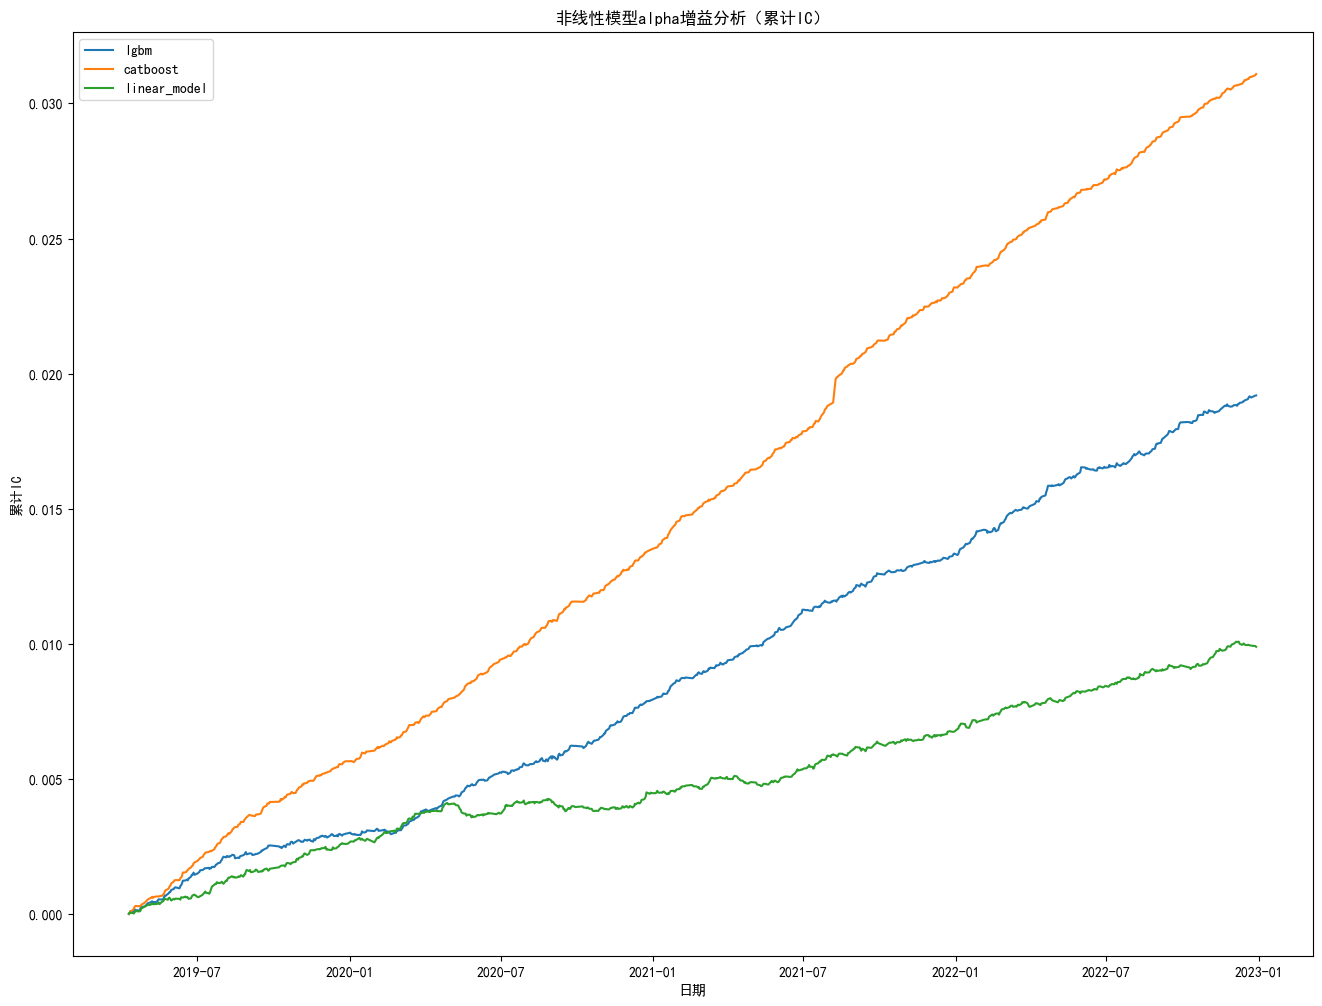
\includegraphics[width=1.15\textwidth]{../Figure/non-linear-insample.png}}
    \caption{非线性模型与线性基准的累积平均IC对比（训练集，样本内：2018年9月至2022年12月）}
    \label{fig:nonlinear_ic}
    \vspace{0.5em}
    \begin{minipage}{0.95\textwidth}
        \small\textit{注：图中展示了 LightGBM、CatBoost 两类非线性模型与滚动 Ridge 回归线性基准模型在训练集区间内的累积平均 IC 曲线。非线性模型的 IC 显著高于线性基准，反映了 GBDT 模型更高的拟合容量。}
    \end{minipage}
\end{figure}

\begin{figure}[htbp]
    \centering
    \makebox[\textwidth][c]{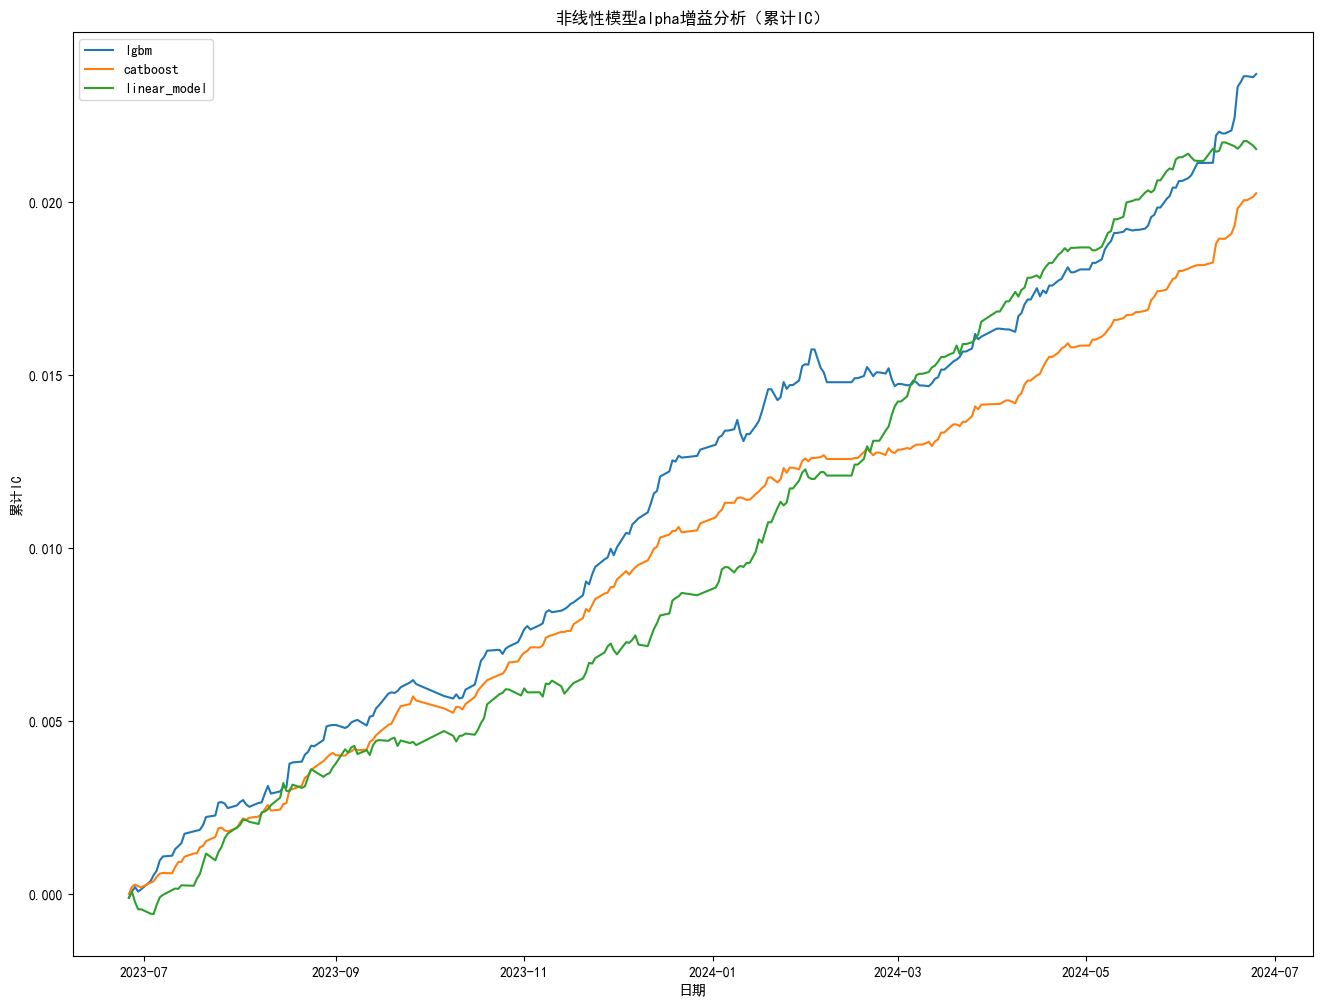
\includegraphics[width=1.15\textwidth]{../Figure/non-linear-outofsample.png}}
    \caption{非线性模型与线性基准的累积平均IC对比（测试集，样本外：2023年6月至2024年6月）}
    \label{fig:nonlinear_sp}
    \vspace{0.5em}
    \begin{minipage}{0.95\textwidth}
        \small\textit{注：图中展示了同一组模型在测试集区间内的累积平均 IC 曲线。与样本内的显著优势形成对比，非线性模型在样本外的 IC 增益几乎可以忽略，LightGBM 和 CatBoost 的表现均与线性基准高度重叠。}
    \end{minipage}
\end{figure}

\subsubsection{结果分析与讨论}

图\ref{fig:nonlinear_ic}和图\ref{fig:nonlinear_sp}的对比揭示了一个重要且值得深入讨论的现象：\textbf{非线性模型在样本内表现远优于线性基准，但在样本外几乎没有实质性的IC增益}。以下从多个维度剖析这一现象的成因。

\vspace{0.3em}
\noindent\textbf{（1）样本内表现差异的解读}

图\ref{fig:nonlinear_ic}中，LightGBM 和 CatBoost 的样本内累积平均IC均显著高于线性基准。这一结果本身并不令人意外：GBDT 作为高容量的非参数集成模型，天然具备捕捉特征与目标之间复杂非线性映射关系的能力——包括特征间的高阶交互效应、特征阈值效应以及局部非单调关系等，这些均为线性模型在函数形式上无法表达的模式。因此，样本内IC的大幅提升主要反映的是\textit{模型容量}（model capacity）的差异，而非可泛化的预测信号质量的本质提升。

\vspace{0.3em}
\noindent\textbf{（2）线性模型滚动训练范式的天然优势}

理解样本外结果之前，需要首先认识到一个关键的方法论差异：线性模型与非线性模型在本文中采用的训练范式存在本质区别。如第\ref{sec:linear_setup}小节所述，线性模型采用滚动在线学习方式，在每个交易日动态更新参数——这意味着线性模型不存在"样本内"与"样本外"的截然划分，其每一天的预测均为真正的样本外预测。因此，线性模型的IC表现不会因数据集边界的变化而出现显著的性能衰减。事实上，从图\ref{fig:nonlinear_sp}中可以观察到，线性模型在测试集区间的IC表现甚至\textit{略优于}训练集区间——这是因为随着滚动训练中累积数据量的持续增加，Ridge 回归的参数估计精度逐步提高，模型的泛化能力也随之增强。换言之，非线性模型在样本外需要超越的"基准线"，是一个经过充分数据训练、参数高度稳定的成熟线性模型，这为非线性模型提出了极高的超越门槛。

\vspace{0.3em}
\noindent\textbf{（3）非线性模型过拟合的深层原因}

非线性模型在样本外未能实现有意义的IC增益，其核心原因在于\textbf{过拟合}。尽管我们在训练中已施加了多项正则化措施（包括随机特征子采样、早停机制、限制树深度和最小叶节点样本数等），但这些措施在本研究的特定数据条件下仍不足以充分抑制过拟合。具体原因如下：

\textit{信噪比极低}：经过残差化处理后的预测目标 bret 已剔除了市场因子、行业因子、市值风格因子和动量因子的全部线性可解释部分，剩余的可预测信号极为微弱——从线性模型日频IC均值约0.012即可窥见，bret 中绝大部分方差来源于不可预测的随机噪声。在如此低的信噪比环境下，非线性模型的高拟合容量反而成为一种负担：模型极易将训练集中的噪声模式（noise pattern）误识别为稳定的信号模式（signal pattern），在统计学习理论中被称为偏差—方差权衡（bias-variance tradeoff）中的高方差端。

\textit{独立特征维度有限}：我们构造的26个特征虽然在运算形式上各有差异，但均基于两个核心原始字段（持仓市值和净持仓变动）派生，且不同半衰期的EMA特征之间、不同归一化方式的特征之间存在显著的\textbf{共线性}。对于线性模型，Ridge 回归的 $L_2$ 正则化天然适合处理高度共线性的特征矩阵，能够在相关特征之间稳定地分配权重。然而，对于树模型，高度相关的特征会导致分裂点选择的不稳定性——在不同的自助法抽样（bagging）或特征子采样中，模型可能选择不同但高度相关的特征进行分裂，从而产生方差较大的集成预测。更为关键的是，当真正独立的信息源有限时，非线性模型难以发掘出线性模型\textit{在本质上无法捕捉}的交互效应或阈值效应，其额外的模型容量更多地被消耗于拟合噪声而非提取信号。

\textit{有效样本量的制约}：非线性模型学习复杂映射关系所需的有效样本量远大于线性模型。虽然名义上训练集包含约4年、数千个交易日乘以数百只股票的观测值，但时间序列上的自相关性意味着\textit{有效独立}样本量远小于名义样本量。在有效样本量有限而模型参数空间较大的条件下，非线性模型本质上处于"欠约束"（under-determined）状态，过拟合几乎是不可避免的。

\vspace{0.3em}
\noindent\textbf{（4）综合评价与未来展望}

综合以上分析，我们得出以下结论：在当前的特征工程框架下，\textbf{线性模型已有效提取了北向资金信息中可稳定预测的线性成分}，而非线性模型未能在样本外展现出实质性的增量贡献。这一结论并不意味着北向资金数据中完全不存在非线性可预测模式，而是表明在现有特征数量和信噪比条件的约束下，非线性模型的额外容量无法被有效利用——其边际收益完全被过拟合成本所抵消。

未来的改进方向可能包括以下几个维度：第一，引入更多\textbf{异质性}的数据源以扩展独立特征维度——例如北向资金的行业配置变化、个股持仓集中度指标、资金流入的日内时间分布特征、沪港通交易额与港股市场指标的联动关系等；第二，采用针对金融时序数据设计的\textbf{时间感知交叉验证}（time-aware cross-validation）和更精细的正则化策略，以更好地控制非线性模型在低信噪比环境中的泛化风险；第三，探索介于线性模型与全非线性 GBDT 之间的\textbf{中间模型形式}——如广义可加模型（Generalized Additive Model, GAM）或带有限交互项的线性模型——以在控制模型复杂度的前提下适度引入非线性表达能力。

\newpage
\section{总结}

本文以沪市A股为研究对象，基于2017年至2025年间的逐股日度持仓与行情数据，从学术与工业双重视角对通过沪深港通渠道进入A股市场的北向资金展开了系统性的实证分析。以下对全文主要发现进行归纳，并指出研究局限与未来改进方向。

\subsection*{主要实证发现}

\textbf{一、北向资金具备显著且稳健的超额收益能力，且以择时为主导。}本文通过构建修正相关系数（式\ref{eq:tilde_coef}）并在HAC稳健框架下完成假设检验，证实北向资金的主动交易行为能够系统性地预测标的股票的短期回报（$\hat{\alpha} = 0.0021$，$t = 3.82$，在1\%水平下显著）。进一步将盈利来源分解为选股收益与择时收益，发现二者贡献分别约为42\%与58\%，以择时为主——即北向资金的信息优势更多体现在对市场整体短期涨跌方向的把握，而非对个股基本面差异的深度挖掘。

\textbf{二、北向资金的交易模式更接近对冲基金而非长线价值投资者。}本文通过构造适用于非对称买卖场景的交易率指标（式\ref{eq:my_turnover}），发现北向资金的日度换手率远超内地机构投资者，甚至与散户投资者的水平相当。这一"对冲基金式"的高频交易特征与市场对北向资金"长线价值配置"的传统认知形成了鲜明反差，并从侧面解释了其择时收益占主导的盈利结构。

\textbf{三、北向资金的预测能力随期限单调递减，仅对短期价格波动具有统计显著的预测力。}多期限截面相关性检验表明，北向资金在日频和月频（1--3个月）预测期限下具有统计显著但经济意义有限的预测能力，而在半年及以上的长期预测期限下预测力完全消失（$t < 1$）。这一发现表明北向资金的信息优势高度集中于短期价格波动的预测，而非对公司基本面内在价值的长期判断，从而从信息结构层面为其可能加剧市场短期波动提供了理论依据。

\textbf{四、北向资金净流入对A股市场存在持续约一周的羊群效应。}基于VAR(4)模型的格兰杰因果检验与脉冲响应函数分析显示，北向资金净流入对沪深港通标的股成交额具有显著的单向引领效应（$F = 15.44$，$p < 0.001$）：当北向资金出现异常净流入冲击时，市场整体成交额在随后约4个交易日内呈现出统计显著的正向响应，之后逐渐衰减至不显著水平。这一约一周的羊群效应与北向资金预测能力集中于短期的发现高度吻合。

\textbf{五、北向资金交易准入的制度性变化导致标的股票收益波动率系统性上升。}以2014年11月17日沪港通正式开通为准自然实验，采用双重差分法（DID）并控制个体与时间固定效应，本文首次系统性地识别出"被纳入沪港通标的"这一处理变量对个股长期波动率的正向因果效应：核心DID系数$\hat{\beta}_3$（Post $\times$ Experiment）在两种波动率指标（$\text{Vol}_1$和$\text{Vol}_2$）、三种控制变量设定下以及剔除事件临近期数据的缩减样本窗口中均在1\%水平下高度显著，且点估计值高度稳定。上述两项发现共同表明，北向资金对A股市场价格发现功能的促进作用有限，其高频交易行为反而系统性地加剧了标的股票的短期波动。

\textbf{六、基于北向资金信息的量化策略实现了高质量的可交易alpha。}针对A股市场因涨跌停板与卖空限制产生大量虚假动量alpha的问题，本文构建了"类Barra"残差化目标体系，通过剔除市场、行业、市值及多时间尺度动量反转因子的线性影响，确保策略alpha与传统动量反转策略在统计上完全正交。在此框架下，基于26个北向资金持仓特征的增量滚动Ridge回归在样本外实现了年化约14.5\%的超额收益、夏普比率接近5.0以及IC均值约0.012的优异表现。alpha信号的ACF半衰期约为0.88个交易日，与北向资金高频交易特征高度吻合，印证了策略的经济逻辑自洽性。

\textbf{七、在当前特征框架与信噪比约束下，非线性模型未能带来样本外增益。}LightGBM与CatBoost两类非线性树模型的测试结果表明，二者在样本内IC显著高于线性基准，但在样本外测试集上的IC增益几乎可忽略。这一结果提示当前特征框架下alpha的可预测成分主要为线性结构，非线性模型的额外容量在低信噪比条件下被过拟合成本所抵消。

\subsection*{研究局限与未来改进方向}

本文的研究存在以下几方面局限，有待后续改进。

\textbf{第一，数据来源的覆盖限制。}本文所使用的北向资金个股持仓数据最早起始于2017年10月，无法覆盖2014年沪港通开通至2017年间的完整历史。这一数据限制使得DID分析与VAR分析所使用的时间窗口无法完全匹配，也限制了对北向资金行为在不同市场周期下演变规律的考察。未来研究可尝试通过替代数据源（如香港联合交易所公布的沪深股通交易数据）填补这一时间缺口。

\textbf{第二，深港通的系统性分析缺失。}本文出于数据完整性考虑，以沪市A股和沪港通为主要研究对象，对深港通及深市A股未进行同等深度的分析。鉴于深市A股中中小市值和成长型标的的比例更高，北向资金在深市的行为模式和市场效应可能与沪市存在系统性差异，对此的深入考察是未来研究的重要方向。

\textbf{第三，策略的可交易性评估尚待完善。}尽管本文在方法论上严格规避了数据泄露问题，并通过残差化框架确保了alpha与动量反转因子的统计正交性，但对策略实际交易成本（冲击成本、市场影响、融券费率等）的定量评估尚不充分。alpha信号约一个交易日的半衰期意味着每日需要大幅换仓，实盘中的执行成本可能对净收益产生显著压缩。未来可在交易模拟器框架下进行更为精细的成本评估。

\textbf{第四，非线性模型的潜力有待进一步挖掘。}当前非线性模型未能带来样本外增益，很可能是特征独立维度不足和数据量相对模型参数空间有限共同作用的结果，而非北向资金信息中本质上不含非线性结构。未来可通过引入更多异质性数据源（如日内交易分布特征、港股市场联动指标、机构情绪指数等）、采用广义可加模型（GAM）等中间形式的模型，以及更精细的时间感知交叉验证策略，进一步探索非线性alpha的可挖掘空间。

\textbf{第五，因果识别框架的潜在局限。}本文DID模型的内部有效性仍依赖于平行趋势假设的成立，即在沪港通开通前，实验组与对照组的波动率变化趋势应当同质。尽管在完整窗口与缩减窗口两组回归中，核心系数均高度稳健，但受限于数据窗口，正式的平行趋势检验（如使用沪港通开通前的多期安慰剂检验）未能在本文中完整呈现。未来研究应在更长的事件前窗口中对平行趋势假设进行更为严格的形式验证。

综合全文的实证发现，本文认为北向资金对A股市场的影响是复杂而双面的：一方面，其主动交易行为确实蕴含着可供挖掘的短期信息增量，为量化策略构建提供了有价值的信号来源；另一方面，其高频择时交易特征与羊群效应的触发机制及标的股票波动率的系统性上升共同表明，北向资金对A股市场价格发现效率的贡献是有限的，其引入在客观上可能使A股市场的短期波动性有所加剧。这一"双刃剑"效应对于监管机构在推进资本市场双向开放过程中制定精准的宏观审慎政策具有直接的参考价值。

\newpage
\nocite{*}
\printbibliography
\end{document}
